\documentclass{amsart}

\usepackage{graphics}

%\usepackage{arxiv}
%\usepackage{enseign}
%\usepackage[utf8]{inputenc} % allow utf-8 input
\usepackage[T1]{fontenc}    % use 8-bit T1 fonts

\usepackage{amsthm}
\usepackage{amsbsy,amsmath,amssymb,amscd,amsfonts}
%\usepackage[pagebackref=true]{hyperref}
\usepackage{hyperref}
\usepackage{url}            % simple URL typesetting
\usepackage{booktabs}       % professional-quality tables
\usepackage{nicefrac}       % compact symbols for 1/2, etc.
\usepackage{microtype}      % microtypography

\usepackage{graphicx,float,latexsym,color}
%\usepackage{refcheck}
%\usepackage{mathspec}
\usepackage[font={small,it}]{caption}
\usepackage{subcaption}
%\let\proof\relax
%\let\endproof\relax

\usepackage{makecell}
\renewcommand{\arraystretch}{1.2}

\usepackage[dvipsnames]{xcolor}

\newtheorem{theorem}{Theorem}
\newtheorem{observation}{Observation}
\newtheorem{proposition}{Proposition}
%\newtheorem{remark}{Remark}

\newtheorem{corollary}{Corollary}
%\newtheorem{definition}{Definition}
\newtheorem{lemma}{Lemma}
\newtheorem{question}{Question}

\theoremstyle{definition}
\newtheorem{definition}{Definition}
\newtheorem{remark}{Remark}
% suggestion of reviewer
%\theoremstyle{definition}
%\newtheorem{definition}{Definition}
%\newtheorem{remark}{Remark}

\hypersetup{
    %bookmarks=true,         % show bookmarks bar?
    %unicode=true,          % non-Latin characters in Acrobat’s bookmarks
    pdftoolbar=true,        % show Acrobat’s toolbar?
    pdfmenubar=true,        % show Acrobat’s menu?
    pdffitwindow=false,     % window fit to page when opened
    pdfstartview={FitH},    % fits the width of 
    colorlinks=true,       % false: boxed links; true: colored links
    linkcolor=OliveGreen,          % color of internal links (change box color with linkbordercolor)
    citecolor=blue,        % color of links to bibliography
    filecolor=black,      % color of file links
    urlcolor=red           % color of external links
}

\usepackage{lineno}
\def\linenumberfont{\normalfont\small\sffamily}
%a4: 210 x 297
%\textwidth=125mm
%\textheight=195mm
\arraycolsep=2pt
\captionsetup{width=120mm}

\title[Circuminvariants of 3-Periodics in the Elliptic Billiard]{Circuminvariants of\\ 3-Periodics in the Elliptic Billiard}

\author{Dan Reznik}


\author{Ronaldo Garcia}


%\author{Jair Koiller}
%\address{Jair Koiller,\\
%Dept. de Matemática,\\
%Univ. Federal de Juiz de Fora,\\
%Juiz de Fora, MG, Brazil}
%\email{jairkoiller@gmail.com}

%\journalname{The Mathematical Intelligencer}
%\journalname{ArXiv}

\begin{document}
\maketitle
%\begin{abstract}
A Circumconic passes through a triangle's vertices; an Inconic is tangent to the sidelines. We study the variable geometry of certain conics derived from the 1d family of 3-periodics in the Elliptic Billiard. Some display intriguing invariances such as aspect ratio and pairwise ratio of focal lengths. We also define the Circumbilliard, a circumellipse to a generic triangle for which the latter is a 3-periodic.

%\vskip .3cm
%\noindent\textbf{Keywords} elliptic billiard, periodic trajectories, triangle center, circumconic, circumellipse, circumhyperbola, conservation, invariance, invariant.
%\vskip .3cm
%\noindent \textbf{MSC} {51M04 \and 37D50  \and 51N20 \and 51N35\and 68T20}
%\end{abstract}

%\begin{abstract}
Can any secrets still be shed by that much studied, uniquely integrable, Elliptic Billiard? Starting by examining the family of 3-periodic trajectories and the loci of their Triangular Centers, one obtains a beautiful and variegated gallery of curves: ellipses, quartics, sextics, circles, and even a stationary point. Secondly, one notices this family conserves an intriguing ratio: Inradius-to-Circumradius. In turn this implies three conservation corollaries: (i) the sum of bounce angle cosines, (ii) the product of excentral cosines, and (iii) the ratio of excentral-to-orbit areas. Monge's Orthoptic Circle's close relation to 4-periodic Billiard trajectories is well-known. Its geometry provided clues with which to generalize 3-periodic invariants to trajectories of an arbitrary number of edges. This was quite unexpected. Indeed, the Elliptic Billiard did surprise us!

\keywords{elliptic billiard, periodic trajectories, integrability, triangle center, locus, loci, conservation, invariance, invariant, constant of motion}

\noindent \textbf{MSC} {37-40, 51N20, 51M04, 51-04}
\end{abstract}

\section{Introduction}
\label{sec:intro}
Given a triangle, a {\em circumconic} passes through its three vertices and satifies two additional constraints, e.g., center or perspector\footnote{Where reference and polar triangles are perspective \cite{mw}.} location. An {\em Inconic} touches each side and is centered at a specified location. Both these objects are associated\footnote{The Isogonal and Isotomic conjugation of such conics are lines \cite[Perspector]{mw}.} with simple lines on the plane \cite[Circumconic,Inconic]{mw} and therefore lend themselves to agile algebraic manipulation.

We study properties and invariants of such conics derived from a 1d family of triangles: 3-periodics in an Elliptic Billiard (EB): these are triangles whose bisectors coincide with normals to the boundary (bounces are elastic), see Figure~\ref{fig:three-orbits-proof}.

Amongst all planar curves, the EB is uniquely integrable \cite{kaloshin2018}. It can be regarded as a special case of Poncelet's Porism \cite{dragovic11}. These two propeties imply two classic invariances: $N$-periodics have constant perimeter and envelop a confocal Caustic. The seminal work is \cite{sergei91} and more recent treatments include \cite{lynch2019-billiards,rozikov2018}. 

\begin{figure}[H]
    \centering
    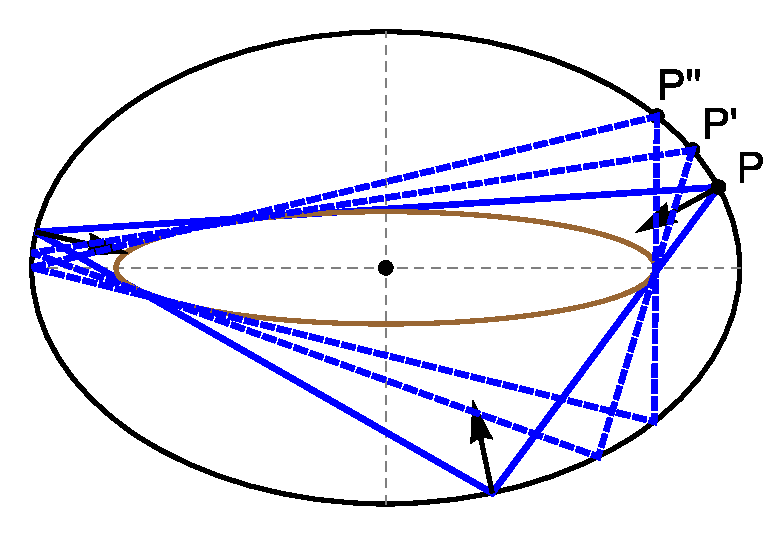
\includegraphics[width=.66\textwidth]{pics_eps_new/0090_three_orbits_proofs.eps}
    \caption{3-periodics (blue) in the Elliptic Billiard (EB, black): normals to the the boundary at vertices (black arrows) are bisectors. The family is constant-perimeter and envelopes a confocal Caustic (brown). This family conserves the ratio inradius-to-circumradius and has a stationary Mittenpunkt at the EB center. \textbf{Video}: \cite[PL\#01]{reznik2020-playlist-circum}.}
    \label{fig:three-orbits-proof}
\end{figure}

We have shown 3-periodics also conserve the Inradius-to-Circumradius\footnote{As does the Poristic Family \cite{gallatly1914-geometry}.} ratio which implies an invariant sum of cosines, and that their {\em Mittenpunkt}\footnote{Where lines drawn from each Excenter thru sides' midpoints meet.} is stationary at the EB center \cite{reznik2020-intelligencer}. Indeed many such invariants have been effectively generalized for $N>3$ \cite{akopyan2020-invariants,bialy2020-invariants}.

We have also studied the loci of 3-periodic Triangle Centers over the family: out of the first 100 listed in \cite{etc}, 29 sweep out ellipses (a remarkable fact on its own) with the remainder sweeping out higher-order curves \cite{garcia2020-ellipses}. Related is the study of  loci described by the Triangle Centers of the Poristic Triangle family \cite{odehnal2011-poristic}.

\textbf{Summary of the paper}: We first describe the {\em Circumbilliard}: the circumellipse associated with a generic triangle for which the latter is a 3-periodic. We then analyze the dynamic of geometry of Circumbilliards for triangles derived from the 3-periodic family such as the Excentral, Anticomplementary, Medial, and Orthic, as well as the loci swept by their centers. We then describe invariants detected for Circumconics and Inconics, namely:

\begin{itemize}
\item Proposition~\ref{prop:right-triangle} in Section~\ref{sec:cb_derived} describes regions of the EB which produce acute, right-triangle, and obtuse 3-periodics. 
\item Theorem~\ref{thm:poristic} in Section~\ref{sec:cb_derived}: The aspect ratio of Circumbilliards of the Poristic Triangle Family \cite{gallatly1914-geometry} is invariant. This is a family of triangle with fixed Incircle and Circumcircle.
    \item Theorem~\ref{thm:axis-ratio} in Section~\ref{sec:circumellipses}: The ratio of semi-axis of Circumellipses centered on the Incenter is invariant over the 3-periodic family. We conjecture this to be the case for a 1d-family of circumellipses.
    \item Theorem~\ref{thm:focal-ratio} in Section~\ref{sec:circumhyperbolae}: The focal lengths of two special circumhyperbola (Feuerbach and Excentral Jerabek) is constant over the 3-periodic family.
    \item Conjectures~\ref{conj:excIncX3} and \ref{conj:excIncX5} in Section~\ref{sec:inconic} claim the aspect ratios of two important Excentral Inconics are invariant. Candidate expressions are provided which match our experiments.
\end{itemize}

A reference table with all Triangle Centers, Lines, and Symbols appears in Appendix~\ref{app:symbols}. Videos of many of the experiments are assembled on Table~\ref{tab:playlist} in Section~\ref{sec:conclusion}.





%\section{Review: Elliptic Billiards}
%\label{sec:billiards}
%\input{002a_review_billiards}
%\newpage

\section{The Circumbilliard}
\label{sec:cb}
Let the boundary of the EB satisfy:

\begin{equation}
\label{eqn:billiard-f}
f(x,y)=\left(\frac{x}{a}\right)^2+\left(\frac{y}{b}\right)^2=1.
\end{equation}

Where $a>b>0$ denote the EB semi-axes throughout the paper. Below we use {\em aspect ratio} as the ratio of an ellipse's semi-axes. When referring to Triangle Centers we adopt Kimberling $X_i$ notation \cite{etc}, e.g., $X_1$ for the Incenter, $X_2$ for the Barycenter, etc., see Table~\ref{tab:kimberling} in Appendix~\ref{app:symbols}.

The following five-parameter equation is assumed for all circumconics not passing through $(0,0)$.

\begin{equation}
1 + c_1 x + c_2 y + c_3 x y + c_4 x^2 + c_5 y^2=0
\label{eqn:e0}
\end{equation}

\begin{proposition}
Any triangle $T=(P_1,P_2,P_3)$ is associated with a unique 
ellipse $E_9$ for which $T$ is a billiard 3-periodic. The center of $E_9$ is T's Mittenpunkt.
\end{proposition}

\begin{proof}
If $T$ is a 3-periodic of $E_9$, by Poncelet's Porism, $T$ is but an element of a 1d family of 3-periodics, all sharing the same confocal Caustic\footnote{This turns out to be the Mandart Inellipse $I_9$ of the family \cite{mw}.}. This family will share a common Mittenpunkt $X_9$ located at the center of $E_9$  \cite{reznik2020-intelligencer}. Appendix~\ref{app:circum-linear} shows how to obtain the parameters for \eqref{eqn:e0} such that it passes through $P_1,P_2,P_3$ and is centered on $X_9$: this yields a $5{\times}5$ linear system. Solving it its is obtained a quadratic equation with positive discriminant, hence the conic is an ellipse.
\end{proof}

$E_9$ is called the Circumbilliard (CB) of $T$. Figure~\ref{fig:circumbilliard} shows examples of CBs for two sample triangles.

\begin{figure}[H]
    \centering
    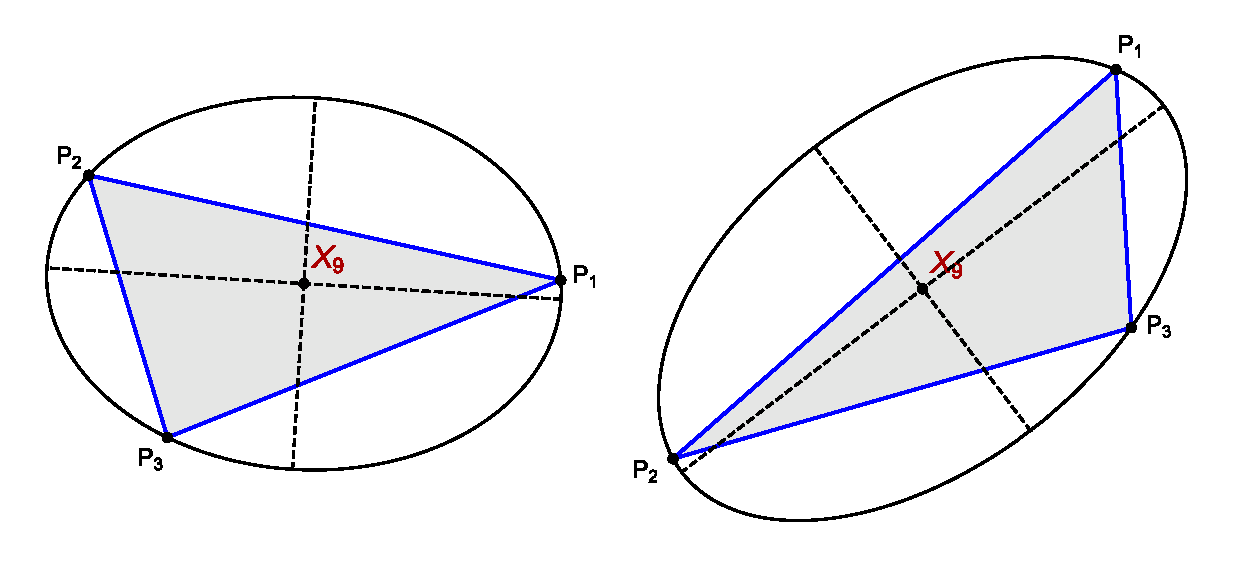
\includegraphics[width=.8\textwidth]{pics_eps_new/0010_circumplot}
    \caption{Two random triangles are shown as well as their Circumbilliards (CBs). Notice their axes in general are not horizontal/vertical. An algorithm for computing the CB is given in Appendix~\ref{app:circum-linear}. \textbf{Video:} \cite[PL\#02]{reznik2020-playlist-circum}}
    \label{fig:circumbilliard}
\end{figure}




\section{Circumbilliards of Derived Triangles}
\label{sec:cb_derived}
Figure~\ref{fig:cb_trio} shows CBs for the Excentral, Anticomplementary (ACT), and Medial Triangles, derived from 3-periodics.

\begin{figure}
    \centering
    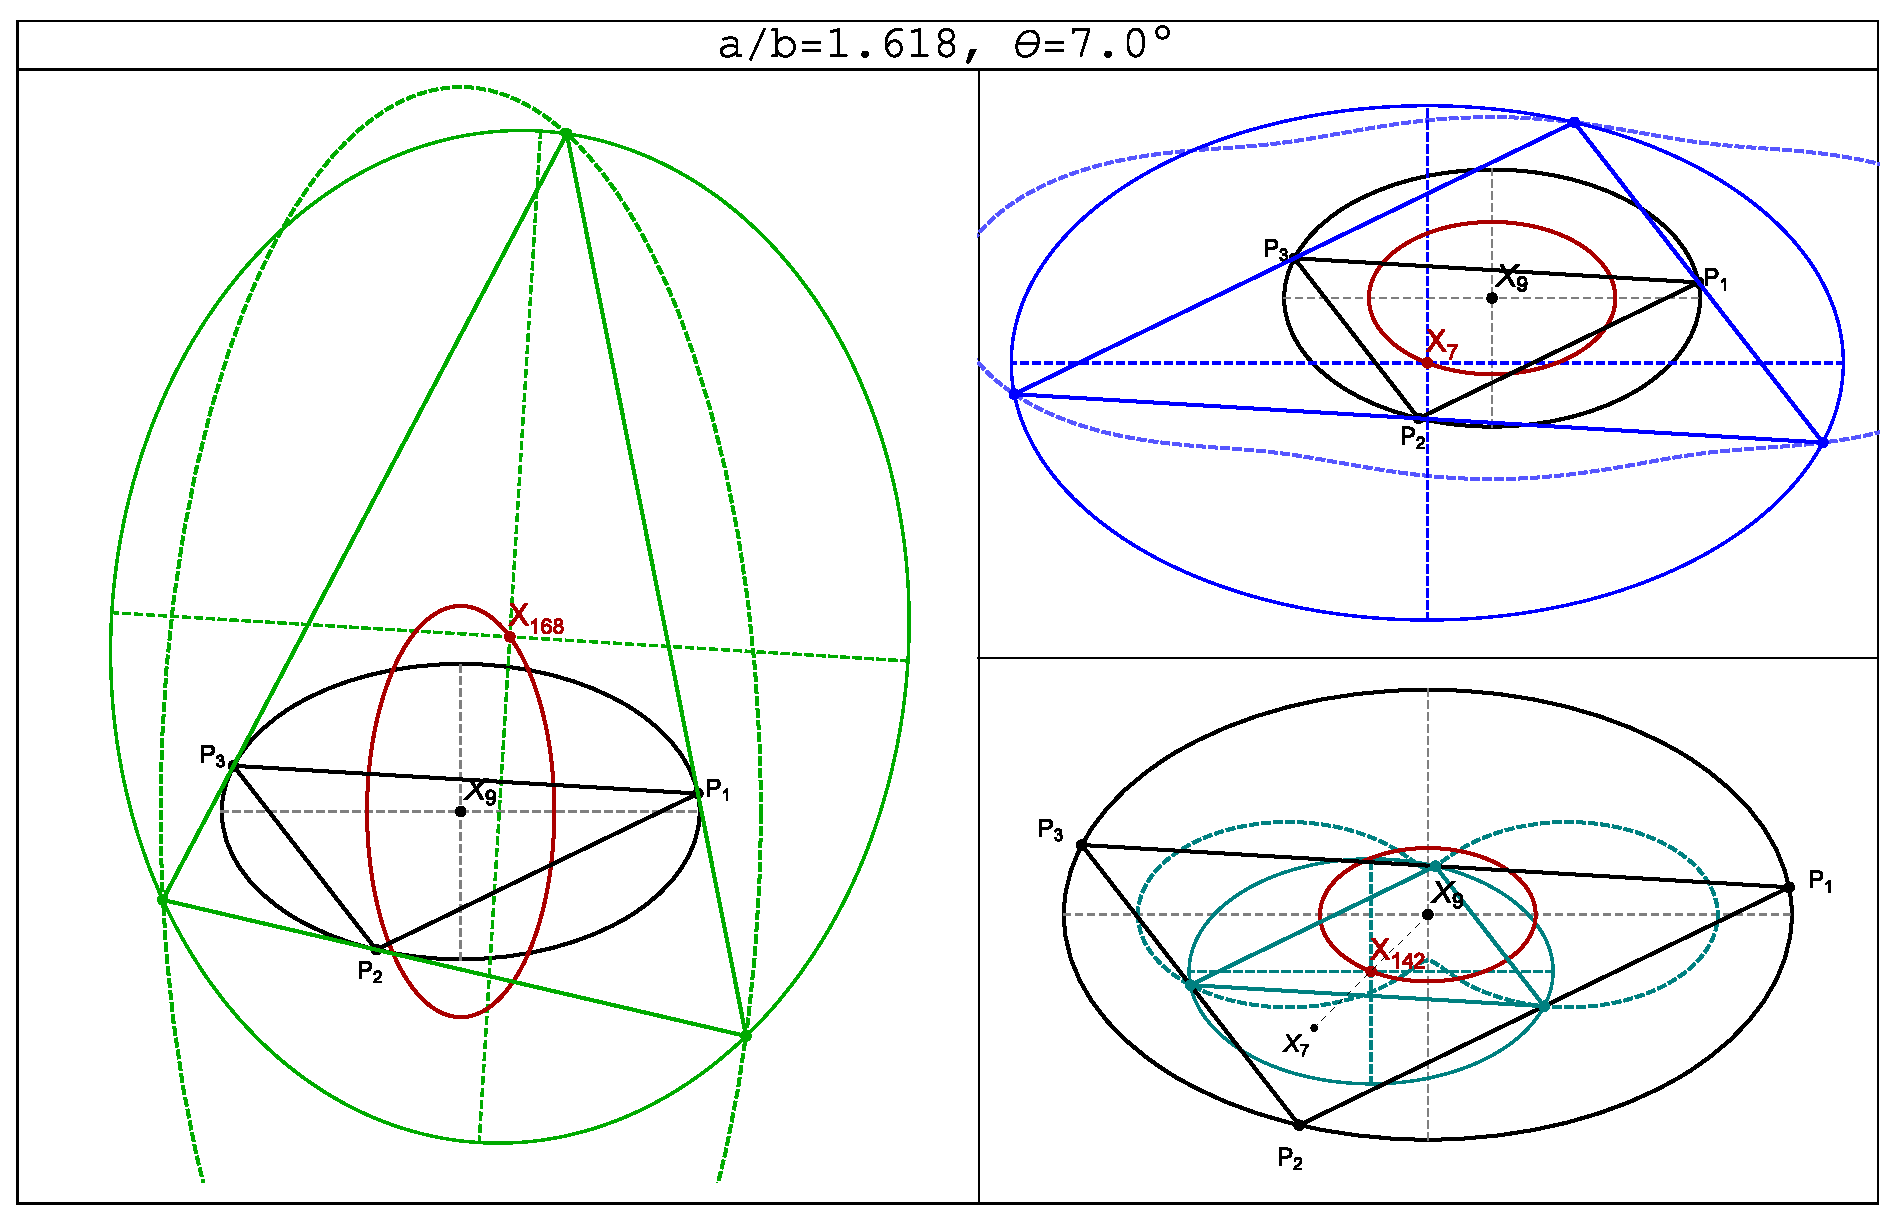
\includegraphics[width=\textwidth]{pics_eps_new/0020_cb_trio.eps}
    \caption{Draw in black in each picture is an $a/b{\simeq}1.618$ EB and a 3-periodic at $t=7.0$ degrees. {\bf Left}: the CB of the Excentral Triangle (solid green) centered on the latter's Mittenpunkt is $X_{168}$ \cite{etc}. Its locus (red) is non-elliptic. Also shown (dashed green) is the elliptic locus of the Excenters (the MacBeath Circumellipse $E_6'$ of the Excentrals \cite{mw}), whose center is $X_9$ \cite{garcia2020-ellipses}. {\bf Top Right}: the CB of the Anticomplementary Triangle (ACT) (blue), axis-aligned with the EB. Its center is the Gergonne Point $X_7$, whose locus (red) is elliptic and similar to the EB \cite{garcia2020-ellipses}. The locus of the ACT vertices is not elliptic (dashed blue). {\bf Bottom Right}: the CB of the Medial Triangle (teal), also axis-aligned with the EB, is centered on $X_{142}$, whose locus (red) is also elliptic and similar to the EB, since it is the midpoint of $X_9X_7$ \cite{etc}. The locus of the medial vertices is a dumb-bell shaped curve (dashed teal). {\bf Video:} \cite[PL\#03]{reznik2020-playlist-circum}}
    \label{fig:cb_trio}
\end{figure}

\subsection{Excentral Triangle}
\label{sec:cb_exc}

The locus of the Excenters is shown in Figure~\ref{fig:cb_trio} (left). It is an ellipse similar to the $90^\circ$-rotated locus of $X_1$ and its axes $a_e,b_e$ are given by \cite{garcia2019-incenter,garcia2020-ellipses}:

\begin{equation*}
 a_e=\frac{{b}^{2}+\delta}{a},\;\;\; 
 b_e=\frac{{a}^{2}+\delta}{b}
\end{equation*}

Where $\delta=\sqrt{a^4-a^2 b^2+b^4}$. 

\begin{proposition}
The locus of the Excenters the stationary MacBeath Circumellipse $E_6'$ \cite{mw} of the Excentral Triangles.
\end{proposition}

\begin{proof}
The center of $E_6'$ is the Symmedian Point $X_6$ \cite[MacBeath Circumconic]{mw}. The Excentral Triangle's $X_6$ coincides with the Mittenpunkt $X_9$ of the reference \cite{etc}. Since over the 3-periodics the vertices of the Excentral lie on an ellipse and its center is stationary, the result follows.
\end{proof}

\begin{proposition}
The Excentral CB is centered on $X_{168}$, whose trilinears are irrational, and whose locus is non-elliptic.
\end{proposition}

\begin{proof}
$X_{168}$ is the Mittenpunkt of the Excentral Triangle \cite{etc} and its trilinears are irrational\footnote{No Triangle Center whose trilinears are irrational on sidelengths has yet been found whose locus under the 3-periodic family is an ellipse \cite{garcia2020-ellipses}.} on the sidelengths. To determine if its locus is an ellipse we use the algebro-numeric techniques described in \cite{garcia2020-ellipses}. Namely, a least-squares fit of a zero-centered, axis-aligned ellipse to a sample of $X_{168}$ positions of the 3-periodic family produces finite error, therefore it cannot be an ellipse.
\end{proof}

This had been observed in \cite{garcia2020-ellipses} for several irrational centers such as $X_i,i=$13--18, as well as many others. Notice a center may be rational but produce a non-elliptic locus, the emblematic case being $X_6$, whose locus is a convex quartic. Other examples include $X_j,j=$19, 22--27, etc.

\subsection{Anticomplementary Triangle (ACT)}
\label{sec:cb_act}

The ACT is shown in Figure~\ref{fig:cb_trio} (top right). The locus of its vertices is clearly not an ellipse.

The ACT is perspective with the reference triangle (3-periodic) at $X_2$ and all of its triangle centers correspond to the anticomplement\footnote{Anticomplement: a 1:2 reflection about $X_2$.} of corresponding reference ones \cite{mw}. The center of the CB of the ACT is therefore $X_7$, the anticomplement of $X_9$. We have shown the locus of $X_7$ to be an ellipse similar to the EB with axes \cite{garcia2020-ellipses}:

\begin{equation*}
\left(a_7,b_7\right)=k\left(a,b\right),\;\;\text{with: }k=\frac{2\delta - {a}^{2}-{b}^{2}}{a^2-b^2}
\end{equation*}

\begin{remark}
The axes of the ACT CB are parallel to the EB and of fixed length.
\end{remark}

This stems from the fact the ACT is homothetic to the 3-periodic.

\subsection{Medial Triangle}

The locus of its vertices is the dumbbell-shaped curve, which at larger $a/b$ is self-intersecting, and therefore clearly not an ellipse, Figure~\ref{fig:cb_trio} (bottom right).

Like the ACT, the Medial is perspective with the reference triangle (3-periodic) at $X_2$. All of its triangle centers correspond to the complement\footnote{Complement: a 2:1 reflection about $X_2$.} of corresponding reference ones \cite{mw}. The center of the CB of the Medial is therefore $X_{142}$, the complement of $X_9$. This point is known to sit midway between $X_9$ and $X_7$.

\begin{remark}
The locus of $X_{142}$ is an ellipse similar to the EB.
\end{remark}

This stems from the fact $X_9$ is stationary and the locus of $X_7$ is an ellipse similar to the EB (above). Therefore its axes will be given by:

\begin{equation*}
\left(a_{142},b_{142}\right)=(a_7,b_7)/2
\end{equation*}

Stemming from homothety of 3-periodic and its Medial:

\begin{remark}
The axes of the Medial CB are parallel to the EB and of fixed length.
\end{remark}

\subsection{Superposition of ACT and Medial}

\begin{proposition}
The Intouchpoints of the ACT (resp. 3-periodic) are on the EB (resp. on the CB of the Medial)
\end{proposition}

\begin{proof}
The first part was proved in \cite[Thm. 2]{reznik2020-ballet}. Because the 3-periodic can be regarded as the ACT of the Medial, the result follows.
\end{proof}

This phenomenon is shown in Figure~\ref{fig:cb_act_med_superposed}. Also shown is the fact that $X_i,i=$7, 142, 2, 9, 144 are all collinear and their intermediate intervals are related as $3:1:2:6$. In \cite{etc_central_lines} this line is known as $L(X_2,X_7)$ or $\mathcal{L}_{663}$. $X_{144}$ is the perspector of the ACT and its Intouch Triangle (not shown).
%\begin{align*}
%a(b - c)(b + c - a)x &+ \\
%b(c - a)(c + a - b)y &+ \\
%c(a - b)(a + b - c)z &= 0
%\end{align*}
%I.e., it is L(663), since
%$$X(663) = a(b - c)(b + c - a) ::$$
%Passes through: 2 7 9 57 63 142 144 226 307 329 527 553 579 672 894 908 1025 1400 1423 1445 1447 1652 1653 1708 1741 1944 2002 2094 2285 2406


\begin{figure}
    \centering
    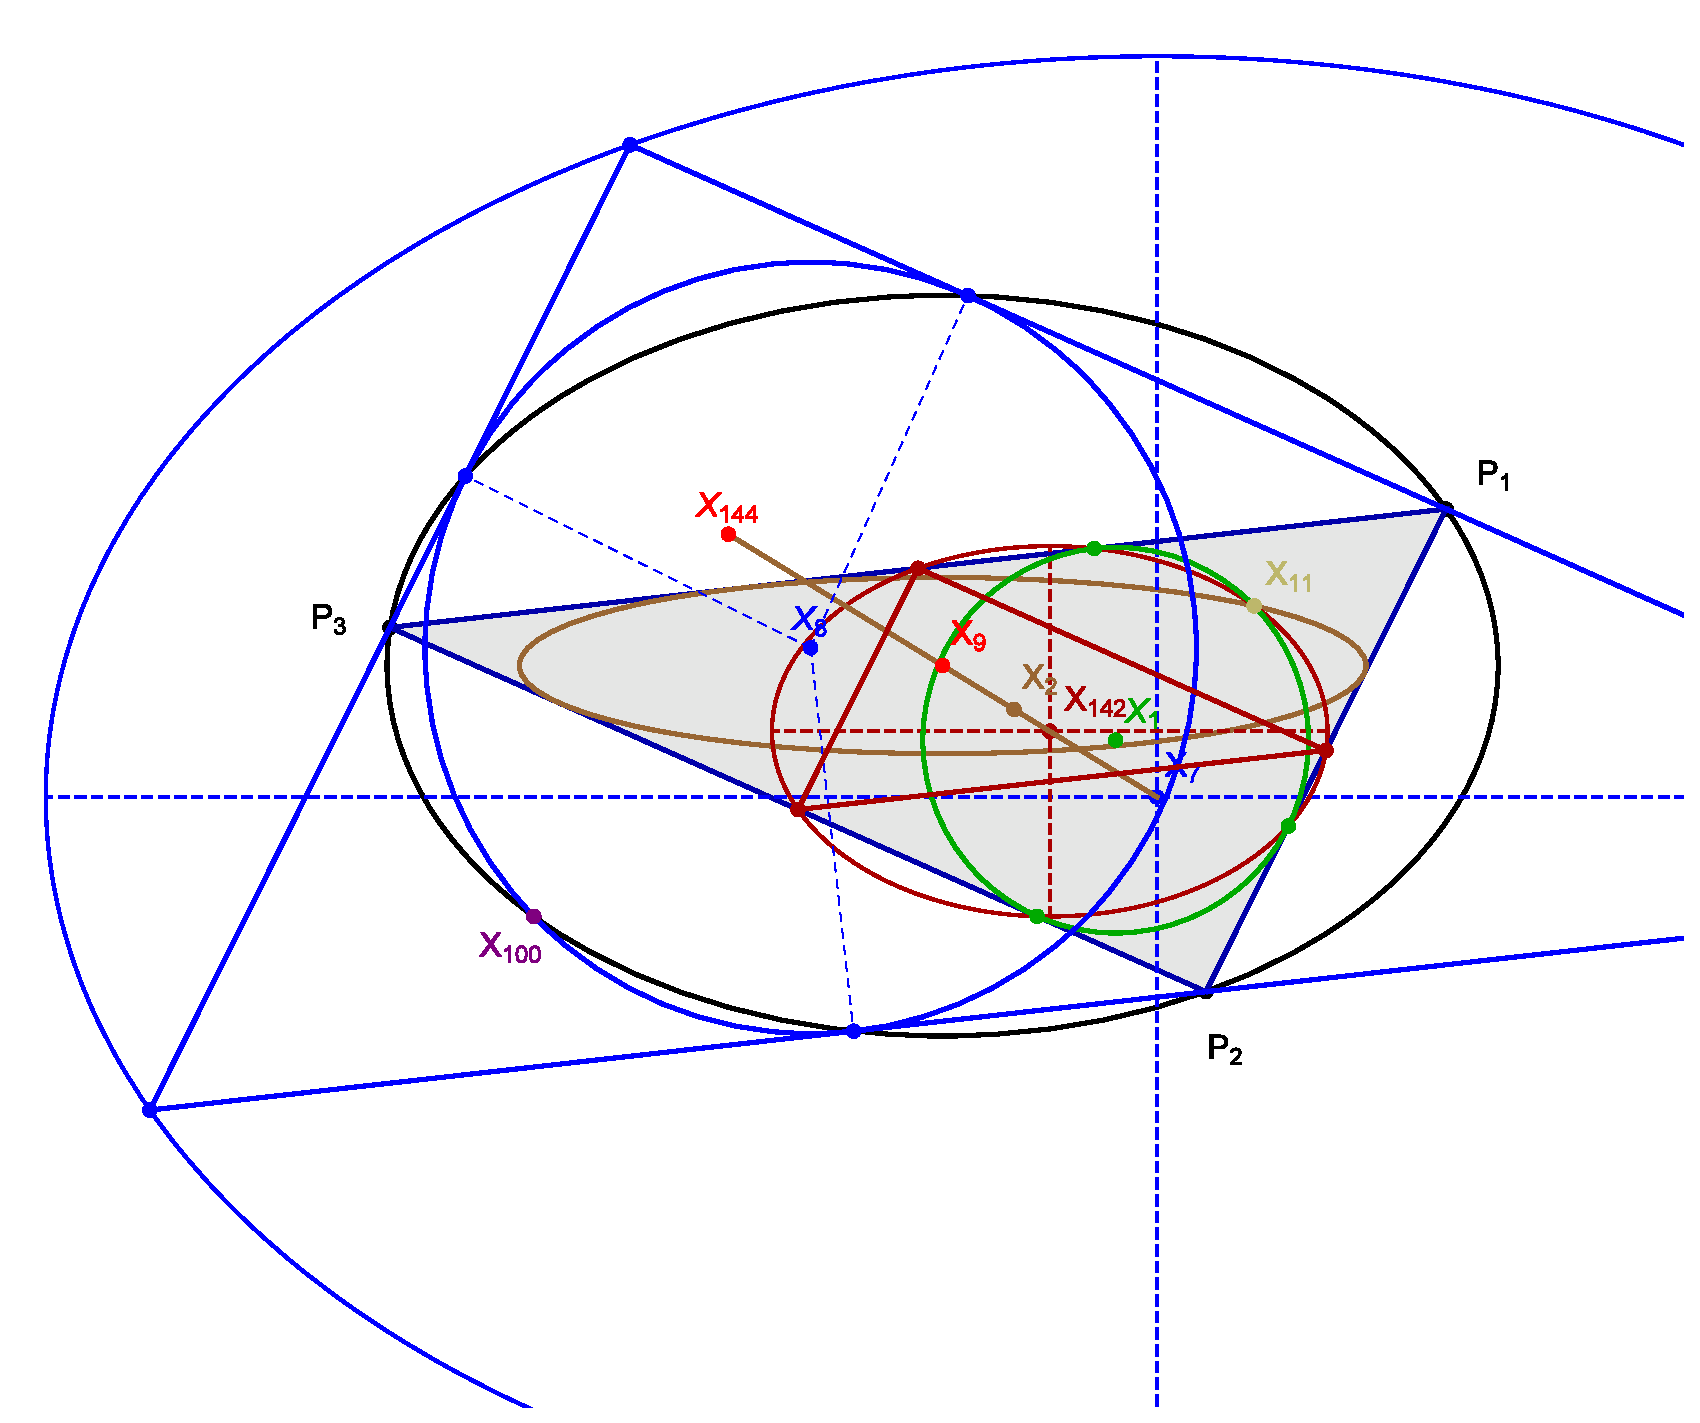
\includegraphics[width=\textwidth]{pics_eps_new/0120_actMedCircumAll.eps}
    \caption{Construction for both ACT and Medial CBs, centered on $X_7$ and $X_{142}$, respectively. The Incircle of the ACT (resp. 3-periodic) is shown blue (resp. green). The former touches the ACT at the EB and the latter touches the 3-periodic sides at the Medial CB. Also shown is line $L(2,7)=L_{663}$ which cointains $X_i$, $i=7,142,2,9,144$. Their consecutive distances are proportional to $3:1:2:6$. $X_{144}$ was included since it is the perspector of the ACT and its Intouch Triangle (not shown) \cite{mw}. \textbf{Video}: \cite[PL\#04,05]{reznik2020-playlist-circum}}
    \label{fig:cb_act_med_superposed}
\end{figure}

\subsection{Orthic Triangle}
\label{sec:cb_ort}

Let $\alpha_4=\sqrt{2\,\sqrt {2}-1}\;{\simeq}\;1.352$. In \cite[Thm. 1]{reznik2020-ballet} we show that if $a/b>\alpha_4$, the 3-periodic family will contain obtuse triangles.

\begin{proposition}
If $a/b>\alpha_4$, the 3-periodic is a right triangle when one of its vertices is at four symmetric points $P^\perp_i$, $i=1,2,3,4$ given by $({\pm}x^\perp,{\pm}y^\perp)$ with:

\begin{equation}
x^\perp=\frac{a^2 \sqrt{a^4+3 b^4-4 b^2 \delta }}{c^3},\;\;\;
y^\perp=\frac{b^2 \sqrt{-b^4-3 a^4+4 a^2 \delta }}{c^3}
\label{eqn:perp}
\end{equation}
\label{prop:right-triangle}
\end{proposition}

\begin{proof}
Let the coordinates of the 3-periodic vertices be $P_1=(x_1,y_1),P_2=(x_2,y_2),P_3=(x_3,y_3)$   as derived in \cite{garcia2019-incenter}.

Computing the equation $\langle P_2-P_1,P_3-P_1\rangle=0$, after careful algebraic manipulations, it follows that $x_1$ satisfies the quartic equation
\[ c^8 x_1^4-2a^4c^2(a^4+3b^4)x_1^2+a^8(a^4+2a^2b^2-7b^4)=0.\] 
For $a/b>\sqrt{2\sqrt{2}-1} $ the only
  positive root in the interval $(0,a)$ is given by

\begin{equation}
x^{\perp}=\frac{a^2 \sqrt{a^4+3 b^4-4 b^2 \delta }}{c^3}.
\label{eqn:xperp}
\end{equation}

\noindent With $y^\perp$ obtainable from \eqref{eqn:billiard-f}.
\end{proof}

Equivalently, a 3-periodic will be obtuse iff one of its vertices lies on top or bottom halves of the EB between the $P_i^\perp$, see Figure~\ref{fig:rect_zones}.

\begin{figure}
    \centering
    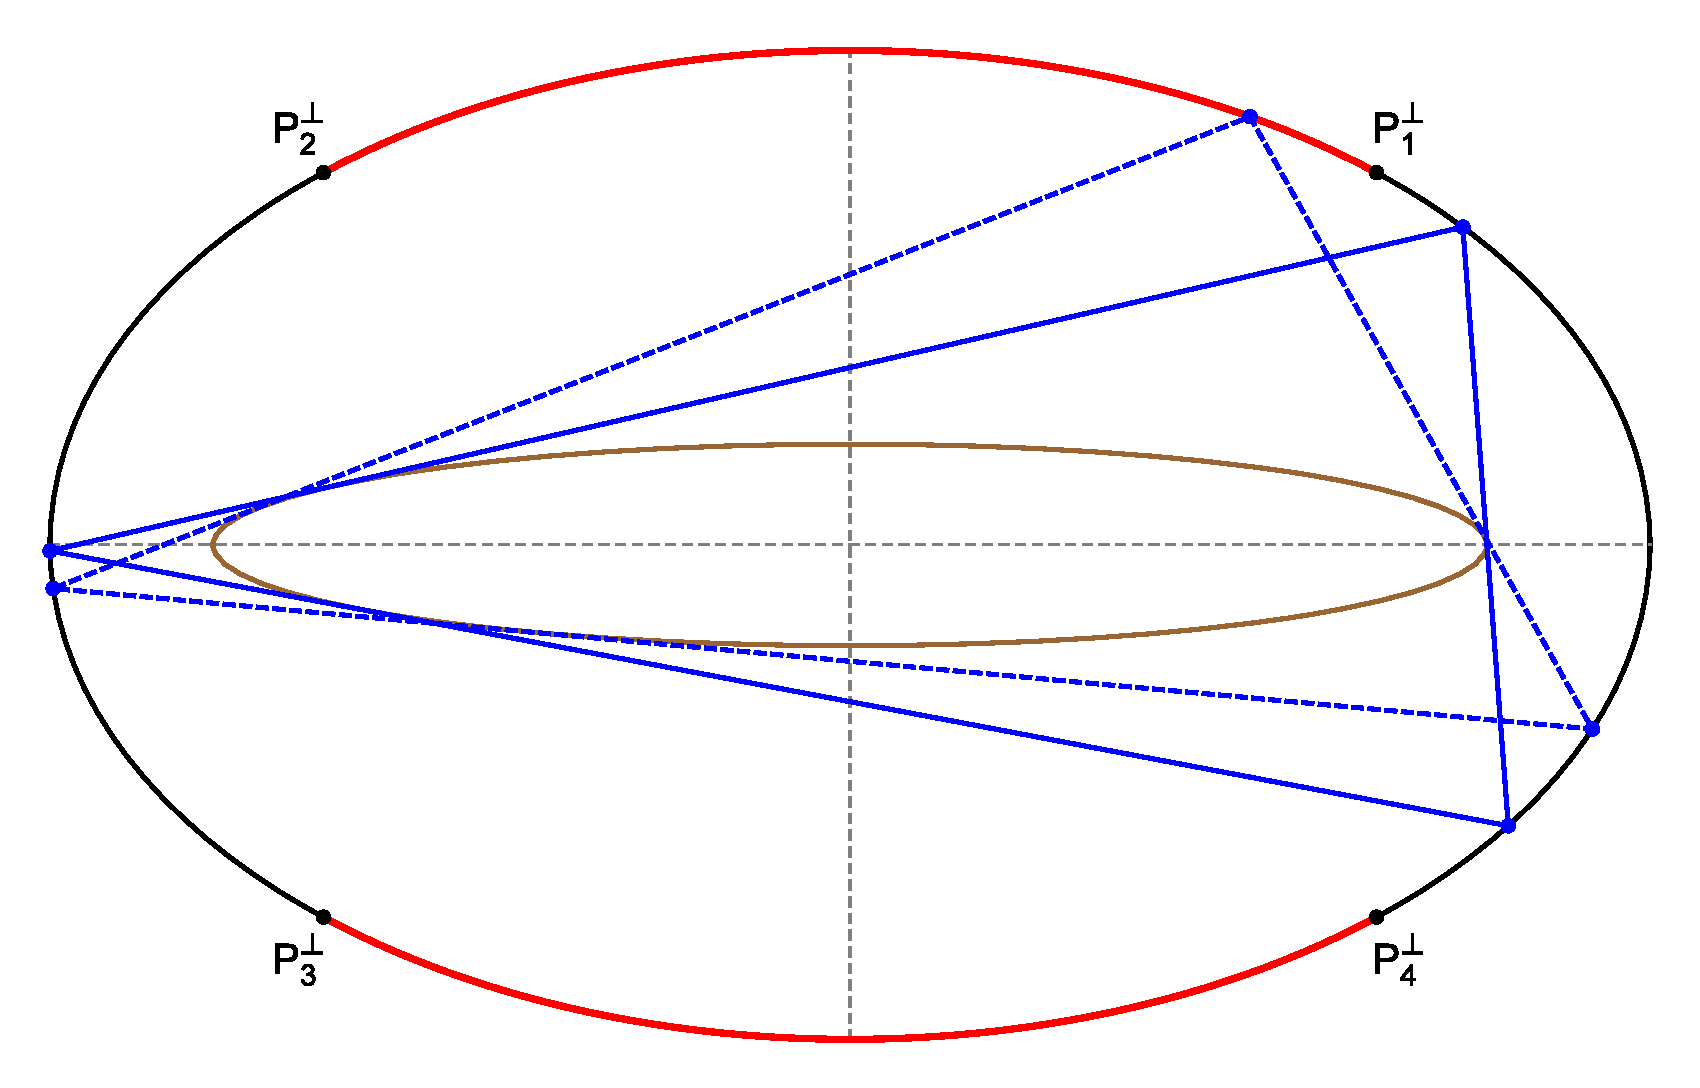
\includegraphics[width=.66\textwidth]{pics_eps_new/0080_rect_zones.eps}
    \caption{Two 3-periodics are shown: one acute (solid blue) and one obtuse (dashed blue) inscribed into an $a/b=1.618$ EB. Red arcs along the top and bottom halves of the EB indicate that when a 3-periodic vertex is there, the 3-periodic is obtuse. These only exist when $a/b>\alpha_4{\simeq}1.352$.}
    \label{fig:rect_zones}
\end{figure}

Consider the elliptic arc along the EB between $({\pm}x^\perp,y^\perp)$. When a vertex of the 3-periodic lies within  (resp. outside) this interval, the 3-periodic is obtuse (resp. acute).

\begin{proposition}
When $a/b>\alpha_4$, the locus of the center of the Orthic CB has four pieces: 2 for when the 3-periodic is acute (equal to the $X_6$ locus), and 2 when it is obtuse (equal to the locus of $X_6$ of $T''=P_2P_3X_4$.
\end{proposition}

\begin{proof}
It is well-known that \cite{etc} an acute triangle $T$ has an Orthic whose vertices lie on the sidelines. Furthermore the Orthic's Mittenpunkt coincides with the Symmedian $X_6$ of $T$. Also known is the fact that:

\begin{remark}
Let triangle $T'=P_1P_2P_3$ be obtuse on $P_1$. Its Orthic has one vertex on $P_2P_3$ and  two others exterior to $T'$. Its Orthocenter $X_4$ is also exterior. Furthermore, the Orthic's Mittenpunkt is the Symmedian Point $X_6$ of acute triangle $T''=P_2P_3X_4$.
\end{remark}

To see this, notice the Orthic of $T''$ is also\footnote{The anti-orthic pre-images of $T'$ are both the 3-periodic and $T''$.} $T'$. $T''$ must be acute since its Orthocenter is $P_2$.
\end{proof}

The CB of the orthic is shown in Figures~\ref{fig:cb_ort} for four 3-periodic configurations in an EB whose $a/b>\alpha_4$.

\begin{proposition}

The coordinates $({\pm}x^*,{\pm}y^*)$ where the locus of the center of the Orthic's CB transitions from one curve to the other are given by:

\begin{align*}
x^*=&\frac{x^{\perp}}{c^6}\left(a^6+2 a^2 b^4- b^2 \delta(3 a^2  +b^2)    +b^6\right)\\
%\frac{a^2 \sqrt{a^4+3 b^4-4 b^2 \delta } \left(a^6+2 a^2 b^4-3 a^2 b^2 \delta +b^6-b^4 \delta \right)}{c^9} \\
%=\frac{a^2 x^{\perp}}{a^2+b^2} \\
y^* =&-\frac{y^{\perp}}{c^6}\left(b^6+2 a^4 b^2 -  a^2 \delta (3 b^2 +a^2)   \delta+a^6\right)
   %\frac{b^2 \sqrt{-3 a^4+4
 %  a^2 \delta -b^4} \left(-a^6-2 a^4 b^2+a^4 \delta +3 a^2 b^2 \delta -b^6\right)}{c^9}\\
  % =\frac{b^2y^{\perp}}{a^2+b^2}
\end{align*}

\end{proposition}

\begin{proof}
Let $P_1=(x_1,y_1)$ be the right-triangle vertex of a 3-periodic, given by $(x^\perp,y^\perp)$ as in \eqref{eqn:xperp}. Using \cite{garcia2019-incenter}, obtain $P_2=(p_{2x}/q_2, p_{2y}/q_2)$ and $P_3=(p_{3x}/q_3, p_{3y}/q_3)$, with:
 
 \begin{align*}
     p_{2x}= &b^4 c^2 x_1^3 -2 a^4 b^2 x_1^2 y_1+a^4 c^2 x_1 y_1^2-2 a^6 y_1^3\\
     %
     p_{2y}=&2 b^6 x_1^3-b^4 c^2  x_1^2 y_1+2 a^2 b^4x_1 y_1^2-a^4 c^2 y_1^3\\
     q_2=&b^4 (a^2+b^2) x_1^2-2 a^2 b^2c^2 x_1 y_1 +a^4 (a^2+b^2) y_1^2\\
     p_{3x}=& b^4 c^2 x_1^3  +2 a^4 b^2 x_1^2 y_1+a^4 c^2 x_1 y_1^2+a^6 y_1^3\\
     p_{3y}=&-2 b^6 x_1^3 -b^4 c^2 x_1^2 y_1-2 a^2 b^4 x_1 y_1^2-a^4 c^2 y_1^3 \\
     q_3=&b^4 (a^2+b^2) x_1^2+2 a^2 b^2c^2 x_1 y_1+a^4 (a^2+b^2) y_1^2
 \end{align*}


It can be shown the Symmedian point $X_6$ of a right-triangle is the midpoint of its right-angle vertex altitude. Computing $X_6$ using this property leads to the result.
\end{proof}

    
Let $\alpha_{eq}=\sqrt{4 \sqrt{3}-3}\,{\simeq}\,1.982$ be the only positive root of $x^4 + 6 x^2 - 39$. It can be shown, see Figure~\ref{fig:cb_ort_equi}:

\begin{proposition}
At $a/b=\alpha_{eq}$, the locus of the Orthic CB is tangent to EB's top and bottom vertices. If a 3-periodic vertex is there, the Orthic is equilateral.
\end{proposition}

\begin{proof}
Let $T$ be an equilateral with side $s_{eq}$ and center $C$. Let $h$ be the distance from any vertex of $T$ to $C$. It can be easily shown that $h/s_{eq}=\sqrt{3}/3$. Let $T'$ be the Excentral Triangle of $T$: its sides are $2s_{eq}$. Now consider the upside down equilateral in Figure~\ref{fig:cb_ort_equi}, which is the Orthic of an upright isosceles 3-periodic. $h$ is clearly the 3-periodic's height and $2s_{eq}$ is its base. The height and width of the upright isosceles are obtained from explicit expressions for the vertices \cite{garcia2019-incenter}:

\begin{align*}
    s_{eq}=\frac{\alpha^2}{\alpha^2-1}\sqrt{2\delta-\alpha^2-1},\;\;\;h=\frac{\alpha^2+\delta+1}{\alpha^2+\delta}
\end{align*}

\noindent where $\alpha=a/b$. Setting $h/s_{eq}=\sqrt{3}/3$ and solving for $\alpha$ yields the required result for $\alpha_{eq}$.
\end{proof}

\begin{figure}
    \centering
    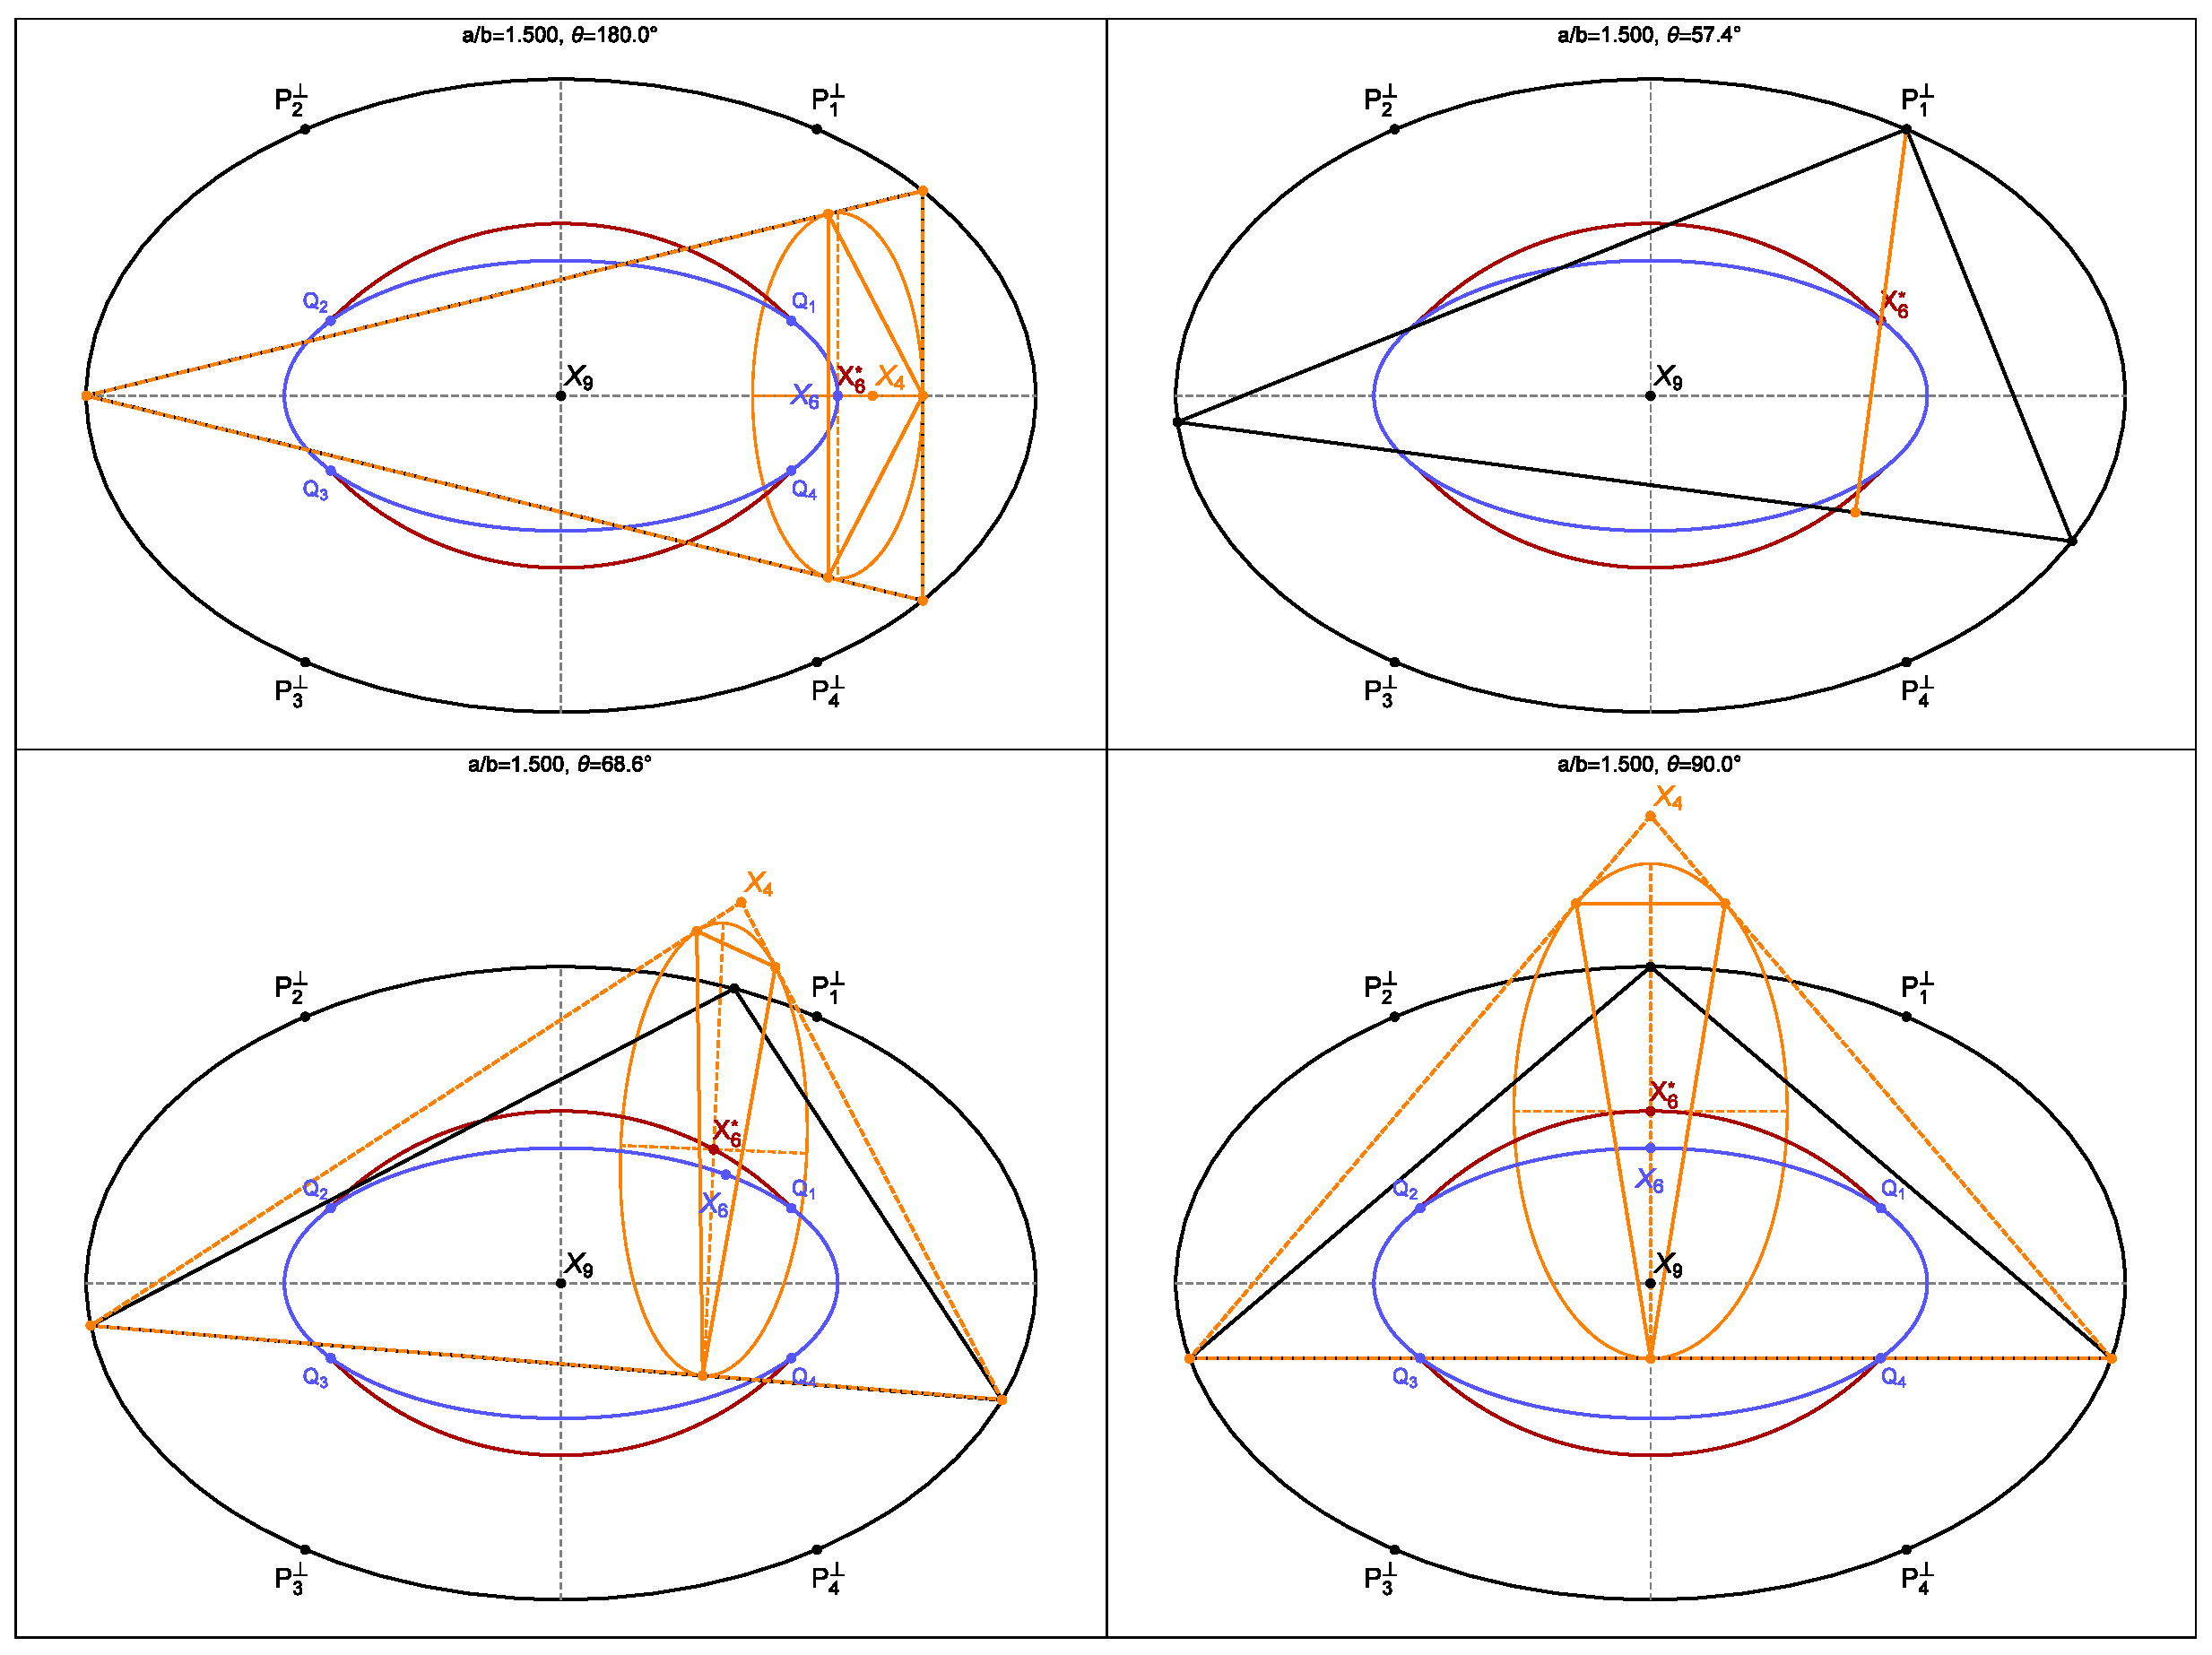
\includegraphics[width=\textwidth]{pics_eps_new/0030_cb_ort.eps}
    \caption{Orthic CB for an EB with $a/b=1.5>\alpha_4$, i.e., containing obtuse 3-periodics, which occur when a 3-periodic vertex lies on the top or bottom areas of the EB between the $P^\perp$. \textbf{Top left}: 3-periodic is sideways isosceles and acute (vertices outside $P^\perp$, so 3 orthic vertices lie on sidelines. The Orthic CB centers is simply the mittenpunkt of the Orthic, i.e, $X_6$ of the 3-periodic (blue curve: a convex quartic \cite{garcia2020-ellipses}). \textbf{Top right}: The position when a vertex is at a $P^\perp$ and the 3-periodic is a right triangle: its Orthic and CB degenerate to a segment. Here the CB center is at a first (of four) transition points shown in the other insets as $Q_i$, $i=1,2,3,4$. \textbf{Bottom left}: The 3-periodic is obtuse, the Orthic has two exterior vertices, and the center of the CB switches to the Symmedian of $T''=P_1P_2X_4$ (red portion of locus). \textbf{Bottom right:}. The 3-periodic is an upright isosceles, still obtuse, the center of the Orthic CB reaches its highest point along its locus (red). \textbf{Video}: \cite[PL\#06]{reznik2020-playlist-circum}.}
    \label{fig:cb_ort}
\end{figure}

\begin{figure}
    \centering
    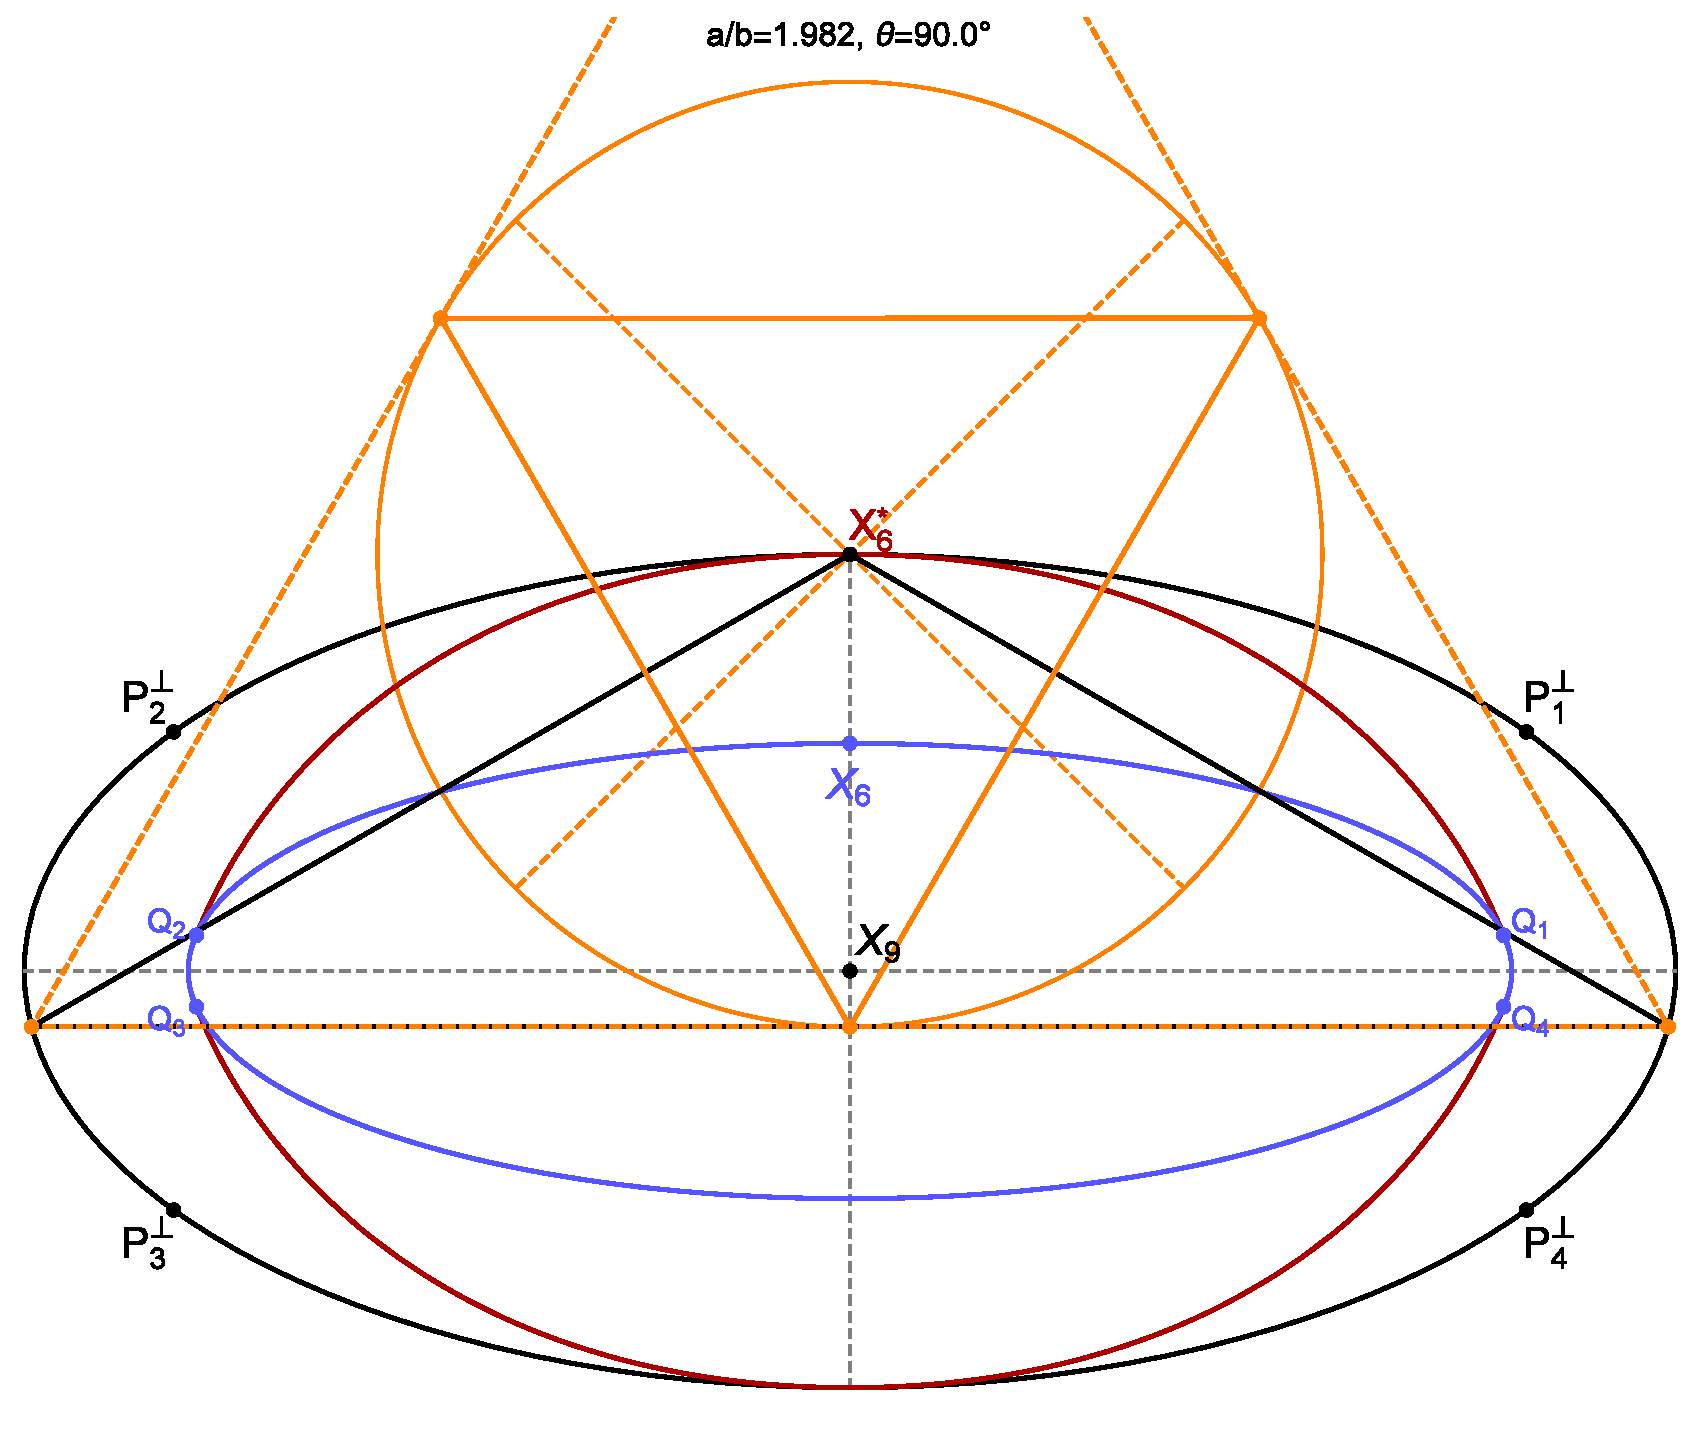
\includegraphics[width=\textwidth]{pics_eps_new/0040_cb_ort_equi.eps}
    \caption{At $a/b=\alpha_{eq}{\simeq}1.982$, the Orthic is an equilateral triangle when a 3-periodic vertex lies on a top or bottom vertex of the EB. Therefore its CB is a circle.}
    \label{fig:cb_ort_equi}
\end{figure}

\subsection{Summary}

Table~\ref{tab:cb_summary} summarizes the CBs discussed above, their centers, and their loci.

\begin{table}[H]
\begin{tabular}{|c|c|c|}
\hline
Triangle & Center & Elliptic Locus \\
\hline
3-Periodic & $X_9$ & n/a \\
Excentral & $X_{168}$ & No\\
ACT & $X_{7}$ & Yes \\
Medial & $X_{142}$ & Yes \\
Orthic & $X_6^*$ & No \\
\hline
\end{tabular}
\caption{CBs mentioned in this Section, their Centers and loci types.}
\label{tab:cb_summary}
\end{table}

\subsection{Circumbilliard of the Poristic Family}

The Poristic Triangle Family is a set of triangles (blue) with fixed Incircle and Circumcircle \cite{gallatly1914-geometry}. It is a cousing of the 3-periodic family in that by definition its Inradius-to-Circumradius $r/R$ ratio is constant.

Weaver \cite{weaver1927-poristic} proved the Antiorthic Axis\footnote{The line passing through the intersections of reference and Excentral sidelines \cite{mw}.} of this family is stationary. Odehnal showed the locus of the Excenters is a circle centered on $X_{40}$ and of radius $2R$ \cite{odehnal2011-poristic}. He also showed that over the family, the locus of the Mittenpunkt $X_9$ is a circle whose radius is $2{d^2}(4R+r)$ and center is $X_1 + (X_1 - X_3) (2 R - r)/(4 R + r)$, where $d=|X_1X_3|=\sqrt{R(R-2{r})}$ \cite[page 17]{odehnal2011-poristic}.

Let $\rho=r/R$ and $a_9,b_9$ be the semi-axis lengths of the Circumbilliard a poristic triangle. As shown in Figure~\ref{fig:cb-poristic}:

\begin{theorem}
The ratio $a_9/b_9$ is invariant over the family and is given by:

\begin{equation*}
\frac{a_9}{b_9}=\sqrt{\frac{\rho^2+2 (\rho+1)\sqrt{1-2\rho} +2}{\rho (\rho+4)}}
\end{equation*}
\noindent where $\rho=r/R$.
\label{thm:poristic}
\end{theorem}

\begin{proof}
The following expression for $r/R$ has been derived for the 3-periodic family of an $a,b$ EB \cite[Equation 7]{garcia2020-new-properties}:

\begin{equation}
  \rho = \frac{r}{R} =  \frac{2(\delta-b^2)(a^2-\delta)}{ (a^2-b^2)^2}
\end{equation}
Solving the above for $a/b$ yields the result.
\end{proof}

\begin{figure}
    \centering
    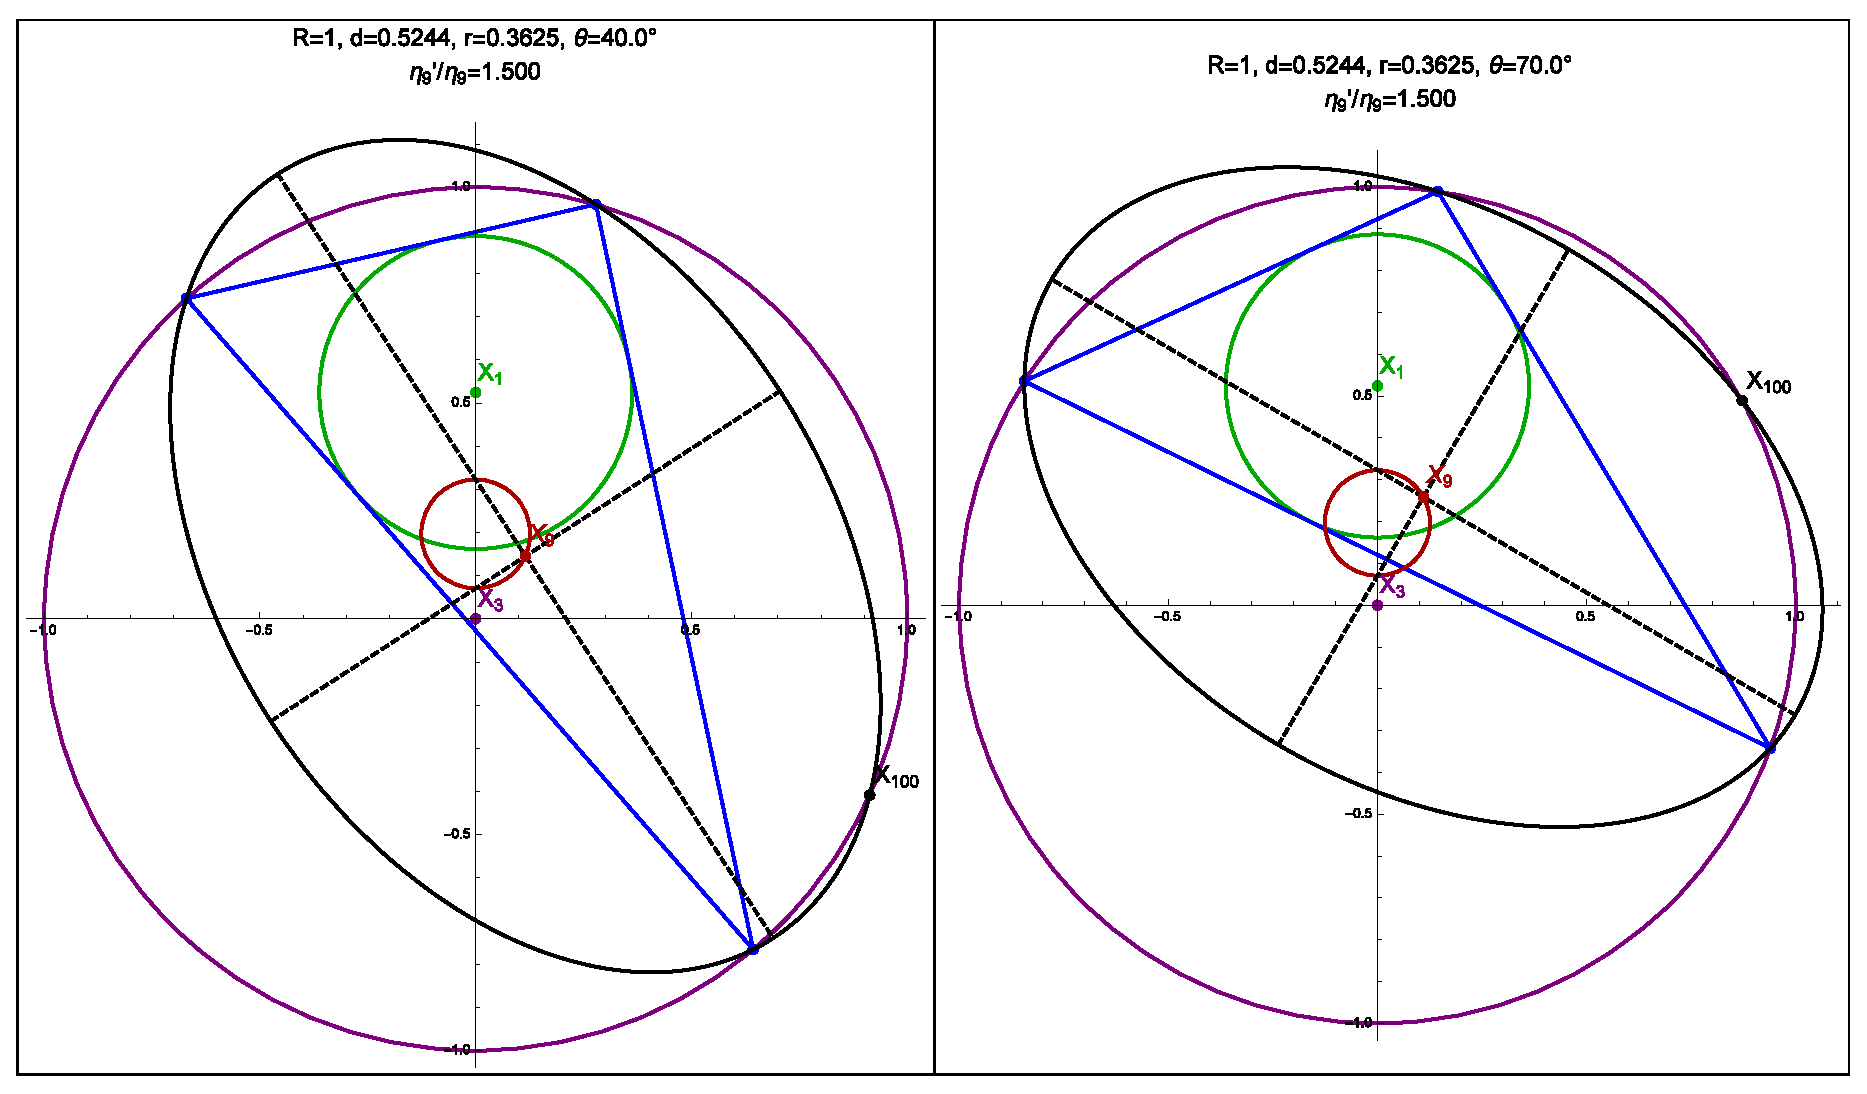
\includegraphics[width=\textwidth]{pics_eps_new/0160_poristic_cb.eps}
    \caption{Two configurations (left and right) of the Poristic Triangle Family (blue), whose Incircle (green) and Circumcircle (purple) are fixed. Here $R=1,r=0.3625$. Over the family, the Circumbilliard (black) has invariant aspect ratio, in this case $a_9/b_9{\simeq}1.5$. Also shown is the circular locus of $X_9$ \cite[page 17]{odehnal2011-poristic}. \textbf{Video}: \cite[PL\#07]{reznik2020-playlist-circum}.}
    \label{fig:cb-poristic}
\end{figure}

\section{Invariants in Circumellipses}
\label{sec:circumellipses}
The Medial Triangle divides the plane in 7 regions, see  Figure~\ref{fig:midlines}. The following is a known fact  \cite{akopyan2007-conics,odehnal2015-conics}:

\begin{remark}
If the center of a Circumconic lies within 4 of these (resp. the remainder 3), the conic will be an Ellipse (resp. Hyperbola).
\end{remark}

\begin{figure}
    \centering
    % used inkspace to go from .pdf -> .eps
    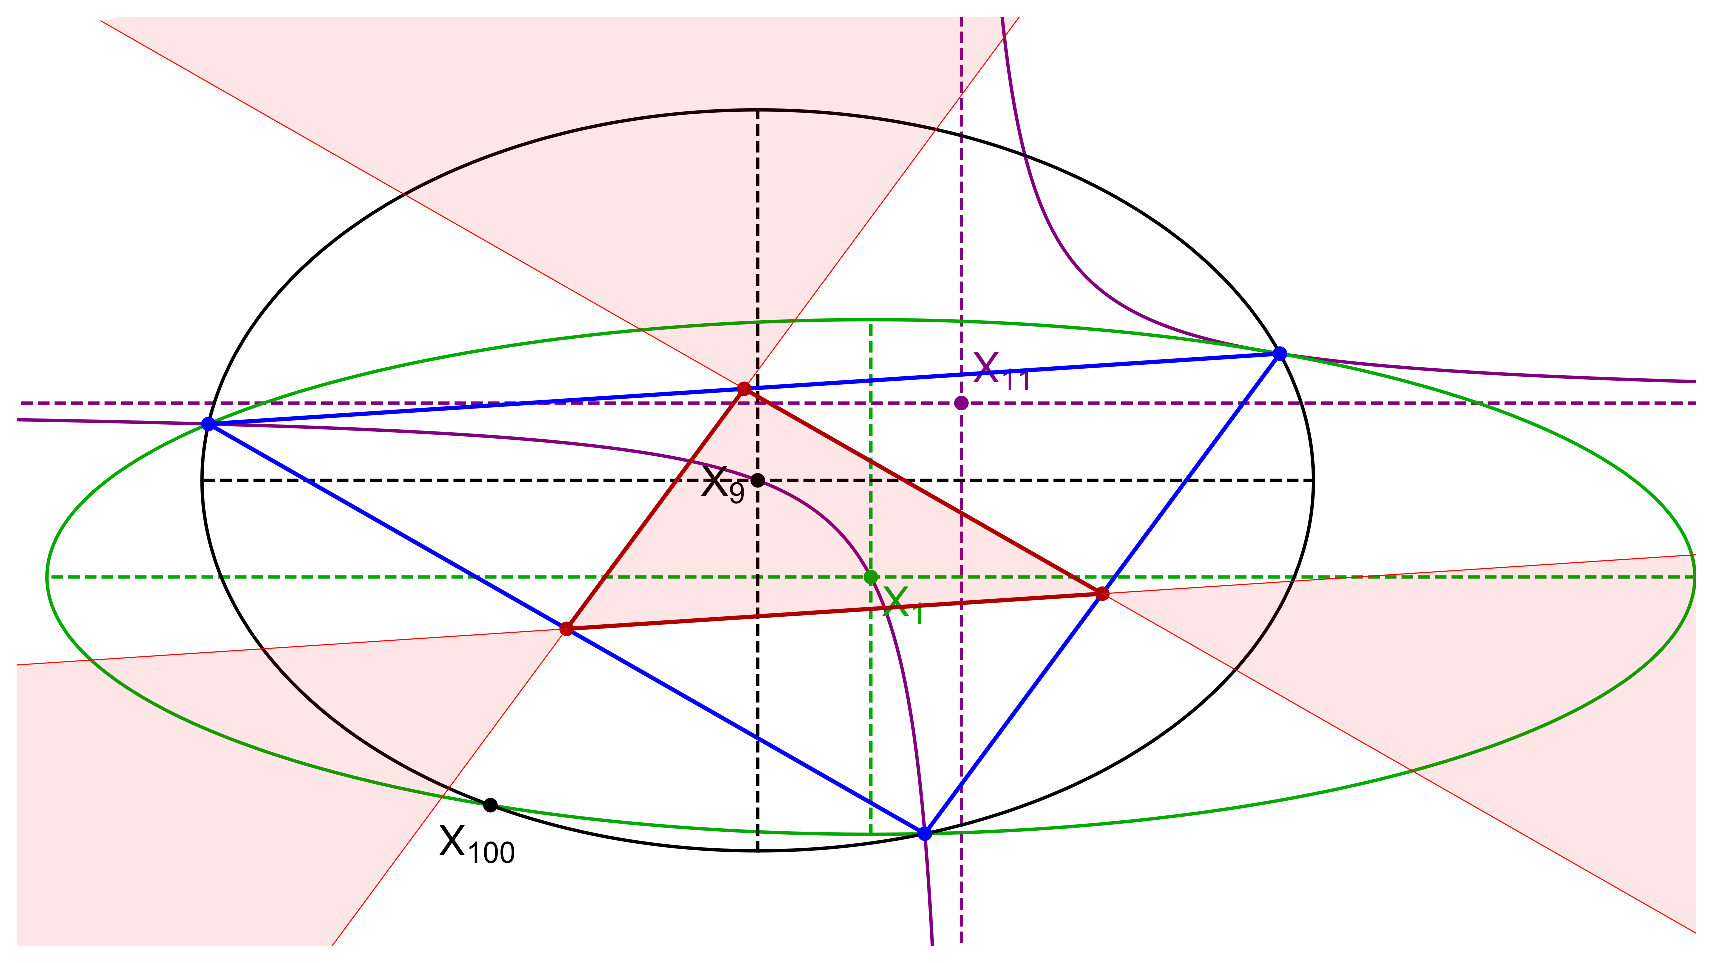
\includegraphics[width=\textwidth]{pics_eps_new/0070_medial_midlines_cropped.eps}
    \caption{A reference triangle is shown (blue) as well as its Medial (red). The latter sides divide the plane into 7 regions, including the Medial' s interior. When a Circumconic center lies on any of the shaded regions (resp. unshaded) it is an Ellipse (resp. Hyperbola). Parabolas have centers at infinity. For illustration, the $X_1$ and $X_9$-centered Circumellipses and the $X_{11}$-centered Feuerbach Hyperbola are shown. Note that over the family of 3-periodics, a given Circumconic may alternate between Ellipse and Hyperbola, e.g., when centered on $X_4$, $X_5$, $X_6$, etc.}
    \label{fig:midlines}
\end{figure}

Centers $X_1$, $X_2$, and $X_9$ are always interior to the Medial Triangle \cite{etc}, so the Circumconics $E_i,i=1,2,9$ centered on them will ellipses, Figure~\ref{fig:circumX1X2}. $E_2$ is the {\em Steiner Circumellipse}, least-area over all possible Circumellipses \cite{mw}, and $E_9$ is $T$'s CB, see Section~\ref{sec:cb}.

It is known that $E_1$ intersects the EB and the Circumcircle at $X_{100}$, the Anticomplement of the Feuerbach Point. Also that $E_2$ intersects $E_9$ at $X_{190}$, the Yff Parabolic Point \cite{dekov14,etc}. These two ellipses intersect at $X_{664}$\footnote{This is the isogonal conjugate of $X_{663}$, i.e., $\mathcal{L}_{663}$ mentioned before is coincidentally its {\em Trilinear Polar} \cite{mw}.} \cite{moses2020-private-circumconic}.

Given a generic triangle $T$:

\begin{proposition}
The axes of $E_1$  are parallel to $E_9$'s. %${e_1}{e_2}={-a^2+2+2\delta}{a^4(2 a^2-1+2\delta)}$.
\end{proposition}

The proof is in Appendix~\ref{app:circum-x1x2x9}. 

\begin{theorem}
Let $\eta_1$ and $\eta_1'$ be the lengths of minor and major semi-axes of $E_1$, respectively. The ratio of their lengths is constant over the 3-periodic family and given by:
\begin{equation*}
\frac{\eta_1'}{\eta_1}=\frac{\sqrt{2\delta^2+2(a^2-b^2)\delta-a^2b^2}}{b^2} >1
\end{equation*}
\label{thm:axis-ratio}
\end{theorem}

%\begin{equation}
%\label{eqn:rovR}
%\frac{r}{R}=\frac{2(\delta-b^2)(a^2-\delta)}{(a^2-b^2)^2}
%\end{equation}

\begin{proof}
Calculate the ratio using vertex locations (see \cite{garcia2020-new-properties}) for an isosceles orbit, and then verify with a Computer Algebra System (CAS) the expression holds over the entire family.
\end{proof}

Note: experimentally $\eta_1'$ is maximal (resp. minimal) when the 3-periodic is an isosceles with axis of symmetry parallel to the EB's minor (resp. major) axis.

\begin{proposition}
The axes of $E_2$ are only parallel to $E_9$ if $T$ is isosceles.
\end{proposition}

See Appendix~\ref{app:circum-x1x2x9}.

%\begin{observation}
%The intersection of %$E_1$ and $E_2$ which is %not a vertex of $T$ is %collinear with $X_{75}$ %and $X_{77}$.
%\end{observation}


% \begin{observation}
%$E_2$ axes are only parallel to the EB's when orbits are isosceles triangles (4 discrete cases). Their lengths $\eta_2$ and $\eta_2'$ are related as $\eta_2 = c_0 + c_1 \eta_2'$, with $c_0,c_1$ constant for all orbits. \textcolor{red}{ronaldo consegue derivar $c_0$ e $c_1$?}
%\end{observation}

\begin{figure}
    \centering
    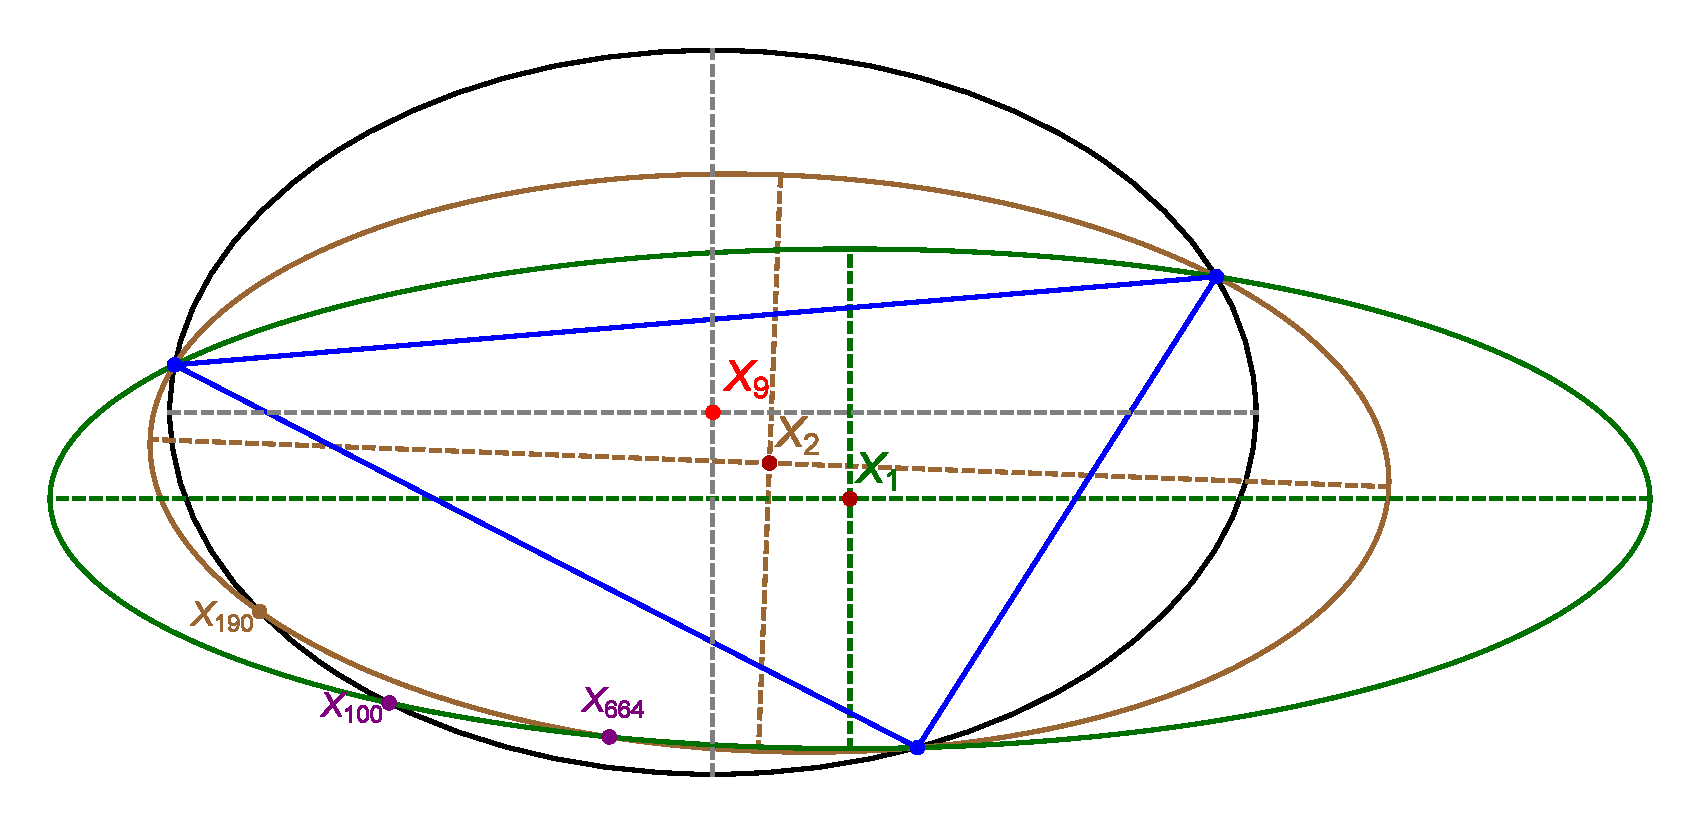
\includegraphics[width=\textwidth]{pics_eps_new/0091_e1e2.eps}
    \caption{$E_1$ (green) and $E_2$ (brown) are Circumellipses to the orbit (blue) centered on $X_1$ (green) and $X_2$ (brown). The former (resp.~latter) intersect the EB at $X_{100}$ (resp.~$X_{190}$). They intersect at the vertices and at $X_{664}$. $E_1$ axes remain parallel to the EB over the orbit family, and the ratio of their lengths is constant. The axes of $E_2$ are only parallel to the EB's when the orbit is an isosceles. \textbf{Video}: \cite[PL\#08]{reznik2020-playlist-circum}.}
    \label{fig:circumX1X2}
\end{figure}

\subsection{Parallel-Axis Pencil}

The Feuerbach Circumhyperbola of a Triangle is a rectangular hyperbola\footnote{Since it passes through the Orthocenter $X_4$ \cite{mw}.} centered on $X_{11}$ \cite{mw}.
Peter Moses has contributed a stronger generalization \cite{moses2020-private-circumconic}:

\begin{remark}
The pencil of Circumconics whose centers lie on the Feuerbach Circumhyperbola $F_{med}$ of the Medial Triangle have mutually-parallel axes. 
\end{remark}

The complement\footnote{The 2:1 reflection of a point about $X_2$.} of $X_{11}$ is $X_{3035}$ \cite{etc} so $F_{med}$ is centered there, see Figure~\ref{fig:circum_parallel}. The following is a list of Circumellipses whose centers lie on $F_{med}$ \cite{moses2020-private-circumconic}: $X_i$,  $i$=1, 3, 9, 10\footnote{Notice $X_{10}$ is the Incenter of the Medial. Interestingly, $X_8$, the Incenter of the ACT, does not belong to this select group.}, 119, 142, 214, 442, 600, 1145, 2092, 3126, 3307, 3308, 3647, 5507, 6184, 6260, 6594, 6600, 10427, 10472, 11517, 11530, 12631, 12639, 12640, 12864, 13089, 15346, 15347, 15348, 17057, 17060, 18258, 18642, 19557, 19584, 22754, 34261, 35204.
%The  results below have been observed experimentally, but still lack a proof.

\begin{proposition}
\label{th:9}
A circumellipse has  center on $F_{med}$ iff it passes through $X_{100}$.
\end{proposition}

A proof appears in Appendix~\ref{app:ce_parallel}. The following has been observed experimentally:

\begin{conjecture}
Over the family of 3-periodics, all Circumellipses in Moses' pencil conserve the ratio of their axes.
\label{conj:moses}
\end{conjecture}

\begin{figure}
    \centering
    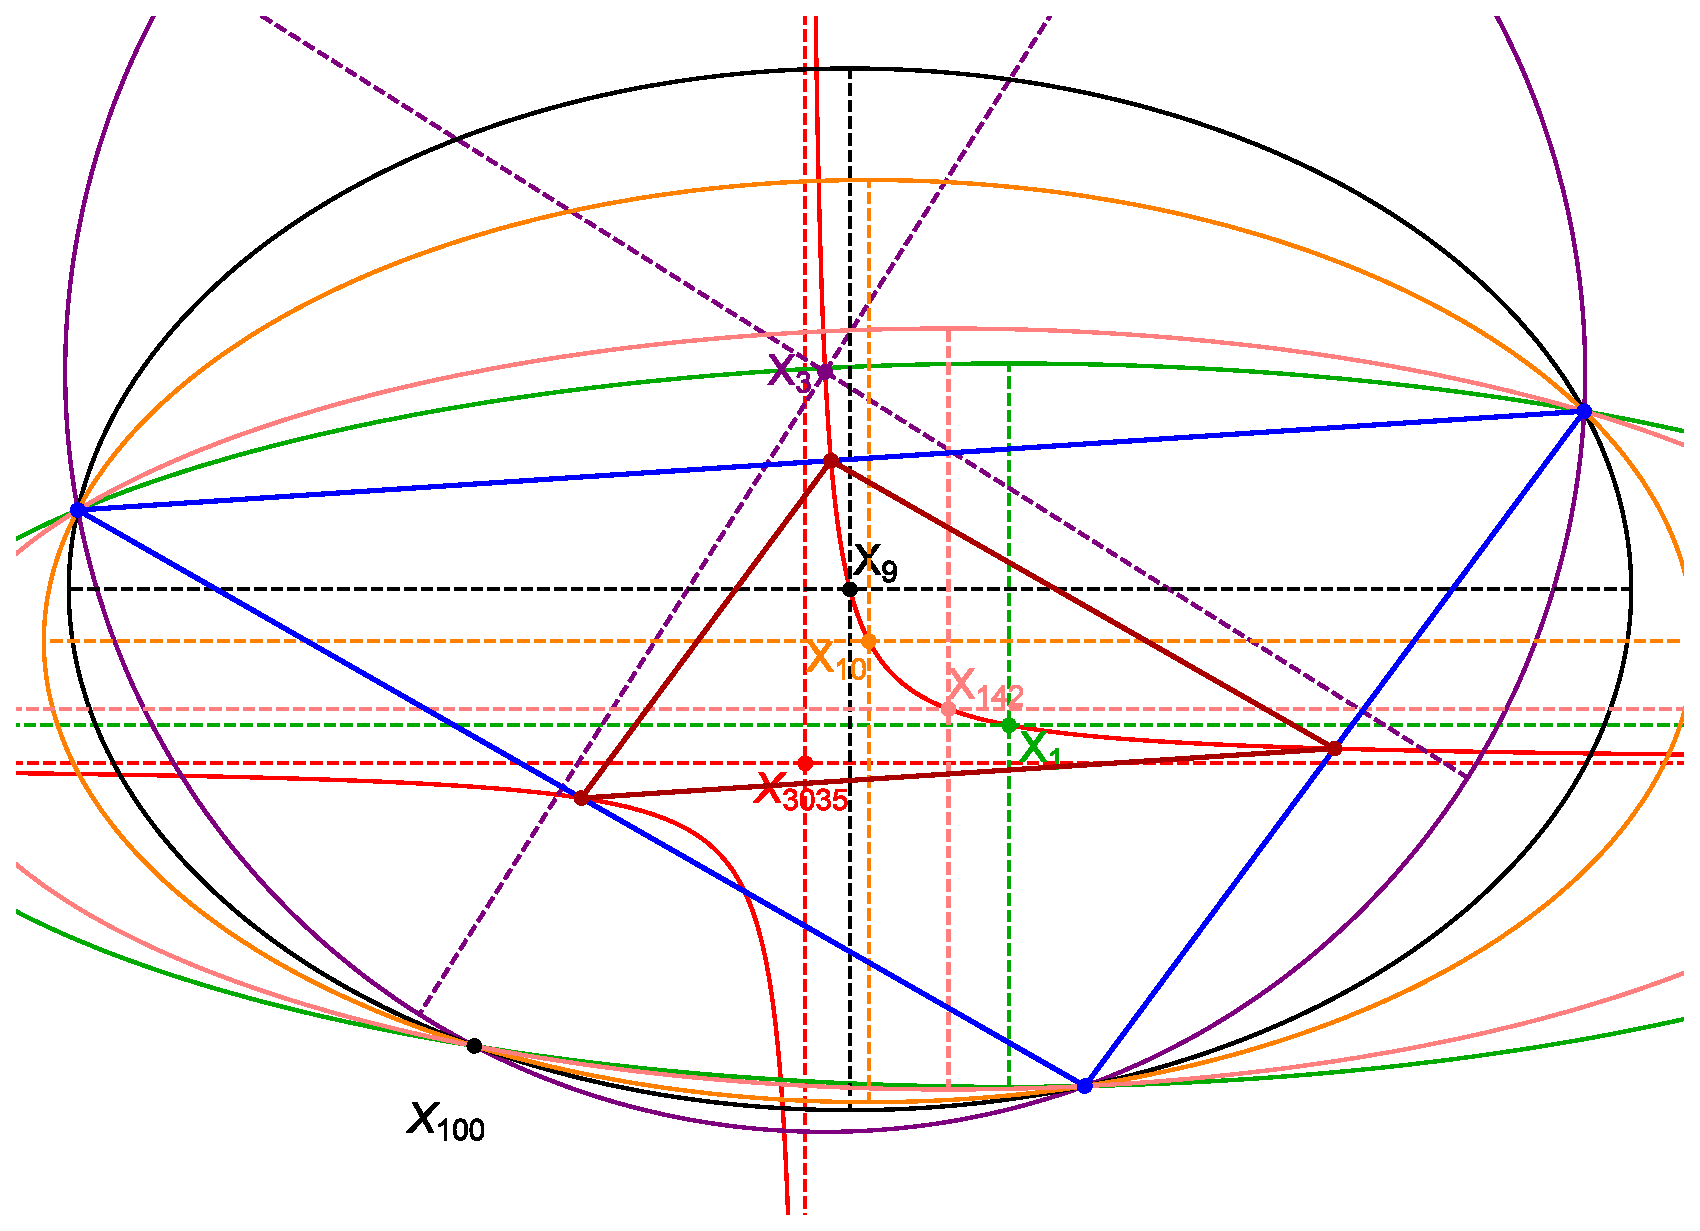
\includegraphics[width=\textwidth]{pics_eps_new/0050_ce_x100.eps}
    \caption{An $a/b=1.5$ EB is shown (black) centered on $X_9$ as well as a sample 3-periodic (blue). Also shown are Circumellipses centered on $X_i$, $i=$1, 3, 10, 142, whose centers lie on the Feuerbach Circumhyperbola of the Medial Triangle (both shown red), centered on $X_{3035}$, the complement of $X_{11}$. Notice all conics drawn (including the Circumhyp). have axes parallel to the EB and all Circumellipses pass through $X_{100}$. Note: the Circumellipse centered on $X_3$ is the Circumcircle, its axes, drawn diagonally, are immaterial.}
    \label{fig:circum_parallel}
\end{figure}

\section{A Special Pair of  Circumhyperbolae}
\label{sec:circumhyperbolae}

Here we study invariants of two well-known Circumhyperbolae\footnote{Its centers lie in the unshaded regions in Figure~\ref{fig:midlines}.}: the Feuerbach and Jerabek Hyperbolas $F$ and $J$ \cite[Jerabek Hyperbola]{mw}. Both are rectangular since they contain $X_4$ \cite{mw}. The former is centered on $X_{11}$ and the latter on $X_{125}$. With respect to 3-periodics no invariants have been detected for $J$. However, the Jerabek $J_{exc}$ of the Excentral Triangle, which passes through the Excenters and is centered on $X_{100}$\footnote{The Excentral's $X_{125}$ \cite{mw}.}, does produce interesting invariants\footnote{The Feuerbach Hyperbola $F_{exc}$ has not yet yielded any detectable invariants over the 3-periodic family.}. 
$F$ is known to pass through $X_1$ and $X_9$ of its reference triangle. Interestingly
$J_{exc}$ also passes through $X_1$ and $X_9$. This stems from the fact that $J$ passes through $X_4$ and $X_6$. Since the Excentral Triangle is always acute \cite{coxeter67}, its $X_4$ is $X_1$. Likewise, the excentral $X_6$ is $X_9$. 

The Isogonal Conjugate of a Circumconic is a line \cite[Circumconic]{mw}. Remarkably:

\begin{remark}
The Isogonal conjugate of $F$ with respect to a reference triangle and that of $J_{exc}$ with respect to the Excentral one is line $X_1X_3=\mathcal{L}_{650}$.
\end{remark}

The first part is well-known \cite[Feuerbach Hyperbola]{mw}. For the second part, consider that $J$ is the Isogonal Conjugate of the Euler Line \cite[Jerabek Hyperbola]{mw}. The Euler Line of the Excentral Triangle passes through its $X_4$ and $X_5$ which are $X_1$ and $X_3$ in the reference 3-periodic.

Referring to Figure~\ref{fig:circumhyps}:

\begin{proposition}
$J_{exc}$ intersects $E_9$ in exactly two locations.
\end{proposition}

\begin{proof}
Let $s_i,i=1,2,3$ refer to 3-periodic sidelengths. The perspector of $J_{exc}$ is $X_{649}=s_1(s_2-s_3)::$ (cyclical) \cite{etc}. Therefore the trilinears $x:y:z$ of $J_{exc}$ satisfy \cite{yiu2003}:
 \[J_{exc}: {s_1(s_2-s_3)}x^2+s_2(s_3-s_1)y^2+s_3(s_1-s_2)z^2=0.\]
 
Notice the above is satisfied for the Excenters $[1:1:-1],\; [1:-1:1]$ and $ [-1:1:1]$. As $X_1=[1:1:1]$ and $X_9=s_2+s_3-s_1::$ (cyclical) it follows that
 $J_{exc}(X_1)=J_{exc}(X_9)=0$.
 
 Eliminating variable $x$, the intersection of $J_{exc}=0$ and $E_9=0$ is given by the quartic:
 
 \begin{align*}
 &s_2(s_1-s_3)k_1 y^4+2s_2(s_1-s_3){k_1}{k_2}y^3 z\\
 +&2s_3(s_1-s_2){k_1}{k_2}y z^3+s_3(s_1-s_2)k_1 z^4=0
 \end{align*}
 
With $k_1=(s_1+s_2-s_3)^2$ and $k_2=s_1+s_3-s_2$. The discriminant of the above equation is:
 
 \[
 -432[(s_2-s_3)(s_1-s_3)(s_1-s_2)(s_1+s_3-s_2)^2(s_1-s_2-s_3)^2(s_1+s_2-s_3)^2(s_1s_2s_3)]^2
 \]
 
Since it is negative, there will be two real and two complex solutions \cite{burnside_1960}.
\end{proof}



\begin{proposition}
$F$ intersects the $X_9$-centered Circumellipse at $X_{1156}$.
\end{proposition}

\begin{proof}
The perspector of $X_9$ is $X_1$ and that of $X_{11} $ is $X_{650}=(s_3-s_3)(s_3+s_3-s_1)::$ (cyclical). Therefore, the trilinears $x:y:z$ of $F$ and $E_9$ satisfy:

\begin{align*}
    F:&(s_2-s_3)(s_2+s_3-s_1)/x+\\
    &(s_3-s_1)(s_3+s_1-s_2)/y+\\
    &(s_1-s_2)(s_1+s_2-s_3)/z=0 \\
    E_9:& 1/x+1/y+1/z=0.
\end{align*} 

$X_{1156}$ is given by $1/[(s_2-s_3)^{2}+s_1( s_2+s_3-2s_1)]::$ (cyclic). This point can be readily checked to satisfy both of the above.
\end{proof}
 
 %abaixo: nao e a Jerabek do excentral e sim do bilhar
%The intersection of $E_9$ with the Jerabek circumhyperbola %$J$ is given by the point
%$X^*=[g(a,b,c):g(b,c,a):g(c,a,b)]$ where
%$g(a,b,c)=(b+c)(a^4 - ( b^2-bc+c^2)a^2-bc(b-c)^2)$. 

Given a generic triangle $T$, the following two claims are known:

\begin{proposition}
The asymptotes of both $F$ and $J_{exc}$ are parallel to the $X_9$-centered circumconic, i.e., $c_4$ and $c_5$ in \eqref{eqn:e0} vanish.
\end{proposition}

\begin{proof}
To see the first part, consider that since the Caustic is centered on $X_9$ and tangent to the 3-periodics, it is the (stationary) Mandart Inellipse $I_9$ of the family \cite{mw}. This inconic is known to have axes parallel to the asymptotes of $F$ \cite{gibert2004-mandart}. Since the Caustic is confocal with the EB, $F$ asymptotes must be parallel to the EB axes.

Secondly, 3-periodics are the Orthic Triangles of the Excentrals, therefore the EB is the (stationary) Excentral's Orthic Inconic \cite{mw}. The latter's axes are known to be parallel to the asymptotes of the Jerabek hyperbola. \cite[Orthic Inconic]{mw}.

An alternate, algebraic proof appears in Appendix \ref{app:circum-x1x2x9}.
\end{proof}

\noindent Let $\lambda$ (resp. $\lambda'$) be the focal length of $F$ (resp. $J_{exc}$).

\begin{remark}
Isosceles 3-periodics have $\lambda'=\lambda=0$.
\end{remark}

To see this consider the sideways isosceles 3-periodic with $P_1=(a,0)$. $P_2$ and $P_3$ will lie on the 2nd and 3rd quadrants at $(-a_c,{\pm}y')$, where $a_c=a(\delta-b^2)/(a^2-b^2)$ is the length of the Caustic major semi-axis \cite{garcia2020-ellipses}. $X_1$ and $X_4$ will lie along the 3-periodic's axis of symmetry, i.e., the x-axis. To pass through all 5 points, $F$ degenerates to a pair of orthogonal lines: the x-axis and the vertical line $x=-a_c$. The foci will collapse to the point $(-a_c,0)$. A similar degeneracy occurs for the upright isosceles, i.e., when $P_1=(0,b)$, namely, the foci collapse to $(0,-b_c)$, where $b_c=b(a^2-\delta)/(a^2-b^2)$ is the Caustic minor semi-axis length.

\begin{theorem}
For all non-isosceles 3-periodics, $\lambda'/\lambda$ is invariant and given by:
\label{thm:focal-ratio}
\end{theorem}
 
\begin{equation}
 \frac{\lambda'}{\lambda}= \frac{\sqrt{\delta^2+\left(a^2+b^2\right)\delta+ a^2b^2}}{a b}=\sqrt{2/\rho}>2
 \label{eqn:focal-ratio}
\end{equation}

\begin{proof}
Assume the EB is in the form of \eqref{eqn:billiard-f}. Let the 3-periodic be given by $P_i=(x_i,y_i),i=1,2,3$. $F$ passes through the $P_i$, $X_1$ and $X_9=(0,0)$. The asymptotes of $F$ are parallel to the EB axes, therefore this hyperbola is given by $c_1x+c_2y+c_3 x y = 0$ and $\lambda^2=|8c_1c_2/c_3^2|$, where: 
\begin{align}
c_1=& y_2y_3(x_2-x_3)x_1^2+(x_2^2y_3-x_3^2y_2-y_2^2y_3
+y_2y_3^2)x_1y_1 \nonumber\\
+&y_2y_3(x_2-x_3)y_1^2  
-(x_2y_3-x_3y_2)(x_2x_3+y_2y_3)y_1
 \nonumber \\
 c_2=&x_2x_3(y_2-y_3)x_1^2+(x_2x_3^2-x_2^2x_3-x_2y_3^2+x_3y_2^2)x_1y_1 \label{eqn:ci} \\
 +&(x_2y_3-x_3y_2)(x_2x_3+y_2y_3)x_1-x_2x_3(y_2-y_3)y_1^2 \nonumber\\
 c_3=& (x_2y_3-x_3y_2)x_1^2+
(x_3^2y_2-x_2^2y_3+  y_2^2y_3-y_2y_3^2)x_1 \nonumber\\
+&(x_3y_2-x_2y_3 )y_1^2 
+(x_2^2x_3-x_2x_3^2+x_2y_3^2-x_3y_2^2)y_1 \nonumber
\end{align}
 
Let $P_i'=(x_i',y_i'),i=1,2,3$ be the Excenters. They are given by
\begin{align} 
    P_1'=&\left({\frac {-{x_1}\,{s_1}+{x_2}\,{s_2}+{x_3}\,{s_3}}{{
s_2}+{s_3}-{s_1}}},{\frac {-{y_1}\,{s_1}+{y_2}\,{
s_2}+{y_3}\,{s_3}}{{s_2}+{s_3}-{s_1}}}\right) \nonumber\\
P_2'=& \left({\frac {{x_1}\,{s_1}-{x_2}\,{s_2}+{x_3}\,{s_3}}{{
s_3}+{s_1}-{s_2}}},{\frac {{y_1}\,{s_1}-{y_2}\,{
s_2}+{y_3}\,{s_3}}{{s_3}+{s_1}-{s_2}}}\right) \label{eqn:pi-prime} \\
P_3'=& \left({\frac {{x_1}\,{s_1}+{x_2}\,{s_2}-{x_3}\,{s_3}}{{
s_1}+{s_2}-{s_3}}},{\frac {{y_1}\,{s_1}+{y_2}\,{
s_2}-{y_3}\,{s_3}}{{s_1}+{s_2}-{s_3}}}\right) \nonumber
\end{align}
Here, $s_1=|P_2-P_3|$, $s_2=|P_1-P_3|$ and $s_3=|P_1-P_2|$.

Since $J_{exc}$ is also centered on the origin and has horizontal/vertical asymptotes, $J_{exc}$ is given by $c_1'x+c_2'y+c_3'x y=0$, and $(\lambda')^2=|8c_1'c_2'/(c_3')^2|$, where $c_i'$ are constructed as \eqref{eqn:ci} replacing $(x_i,y_i)$ with $(x_i',y_i')$.

Consider a right-triangle\footnote{We found this to best simplify the algebra.} 3-periodic, e.g., with $P_1$ at $(x^\perp,y^\perp)$ given in \eqref{eqn:perp} and $P_2$ and $P_3$ obtained explicitly \cite{garcia2019-incenter}. From these obtain $c_i$ using \eqref{eqn:ci}. Using \eqref{eqn:pi-prime} obtain $P_i'$ and the $c_i'$. Finally, obtain a symbolic expression for $\lambda'/\lambda$. After some manipulation and simplification with a Computer Algebra System (CAS), we obtain \eqref{eqn:focal-ratio} which we call a {\em candidate}.

Parametrize the 3-periodic family with $P_1(t)=(a\cos{t},b\sin{t})$ and using the sequence above arrive at an expression for $\lambda'/\lambda$ in terms of $t$. Subtract that from the right-triangle candidate. After some algebraic manipulation and CAS simplification verify the subtraction vanishes, i.e., $\lambda'/\lambda$ is independent of $t$.
\end{proof}

\begin{figure}
    \centering
    \includegraphics[width=\textwidth]{pics_eps_new/0060_circumhyps.eps}
    \caption{An $a/b=1.5$ EB is shown (black) as well as a sample 3-periodic (blue), the confocal Caustic (brown), and the Excentral Triangle (green). The 3-periodic's Feuerbach Circumhyperbola $F$ (orange) passes through its three vertices as well as $X_1$, $X_9$, and $X_4$. The Excentral's Jerabek Circumhyperbola $J_{exc}$ (purple) passes through the three Excenters, as well as $X_1$, $X_9$ and $X_{40}$ (not shown). Two invariants have been detected over the orbit family: (i) the asymptotes (dashed) of both $F$ and $J_{exc}$ stay parallel to the EB axes, (ii) the ratio of focal lengths is constant (focal axis appears dashed). $F$ intersects the Billiard at $X_{1156}$.}
    \label{fig:circumhyps}
\end{figure}

\subsection{Focal Length Extrema}

Let $P_1(t)=(a\cos{t},b\sin{t})$. While their ratio is constant, $\lambda$ and $\lambda'$ undergo three simultaneous maxima in $t\in(0,\pi/2)$, see Figure~\ref{fig:focal-ratio}. In fact, the following additional properties occur at configurations of maximal focal length (we omit the rather long algebraic proofs), see Figure~\ref{fig:zero-hyps}:

\begin{itemize}
    \item $F'$ is tangent to the Caustic at ${\pm}X_{11}$.
    \item $J'_{exc}$ is tangent to the EB at ${\pm}X_{100}$, i.e., at ${\mp}X_{1156}$ (see below).
    %\item $k'_J=a/b$.
\end{itemize}

\begin{remark}
Like $F$, $J'_{exc}$ intersects the EB at $X_{1156}$.
\end{remark}

This happens because $X_{1156}$ is the reflection of $X_{100}$ about $X_9$. If the latter is placed on the origin, then $X_{1156}=-X_{100}$, and $J'_{exc}$ passes through ${\pm}X_{100}$.

Let $F'$ and $J'_{exc}$ be copies of $F$ and $J_{exc}$ translated by $-X_{11}$ and $-X_{100}$ respectively, i.e., they become concentric with the EB (focal lengths are unchanged). Since their asymptotes are parallel to the EB axes and centered on the origin, their equations will be of the form:

\[
F': x\,y = k'_F,\;\;J'_{exc}: x\,y = k'_J
\]

\begin{remark}
$\lambda=2\sqrt{2k'_F}$, $\lambda'=2\sqrt{2k'_J}$, $\lambda'/\lambda=\sqrt{k'_J/k'_F}=\sqrt{2/\rho}$.
\end{remark} 

\begin{figure}
    \centering
    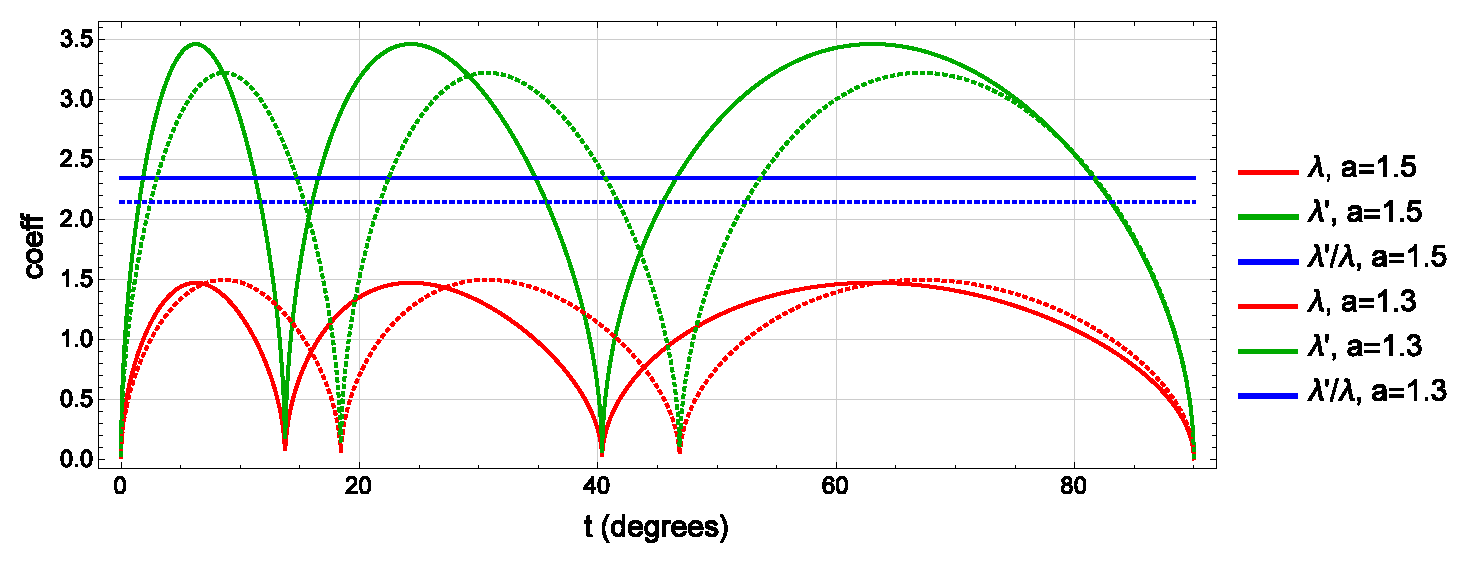
\includegraphics[width=\textwidth]{pics_eps_new/0110_hyp_focals.eps}
    \caption{Focal lengths $\lambda,\lambda'$ of $F,J_{exc}$ vs the parameter $t$ in $P_1(t)=(a\cos{t},b\sin{t})$ are shown red and green. The solid (resp. dasheD) curves correspond to $a/b=1.5$ (resp. $a/b=1.3$). In the first quadrant there are 3 maxima. $\lambda'/\lambda$ (blue) remain constant for the whole interval.}
    \label{fig:focal-ratio}
\end{figure}

\begin{figure}
    \centering
    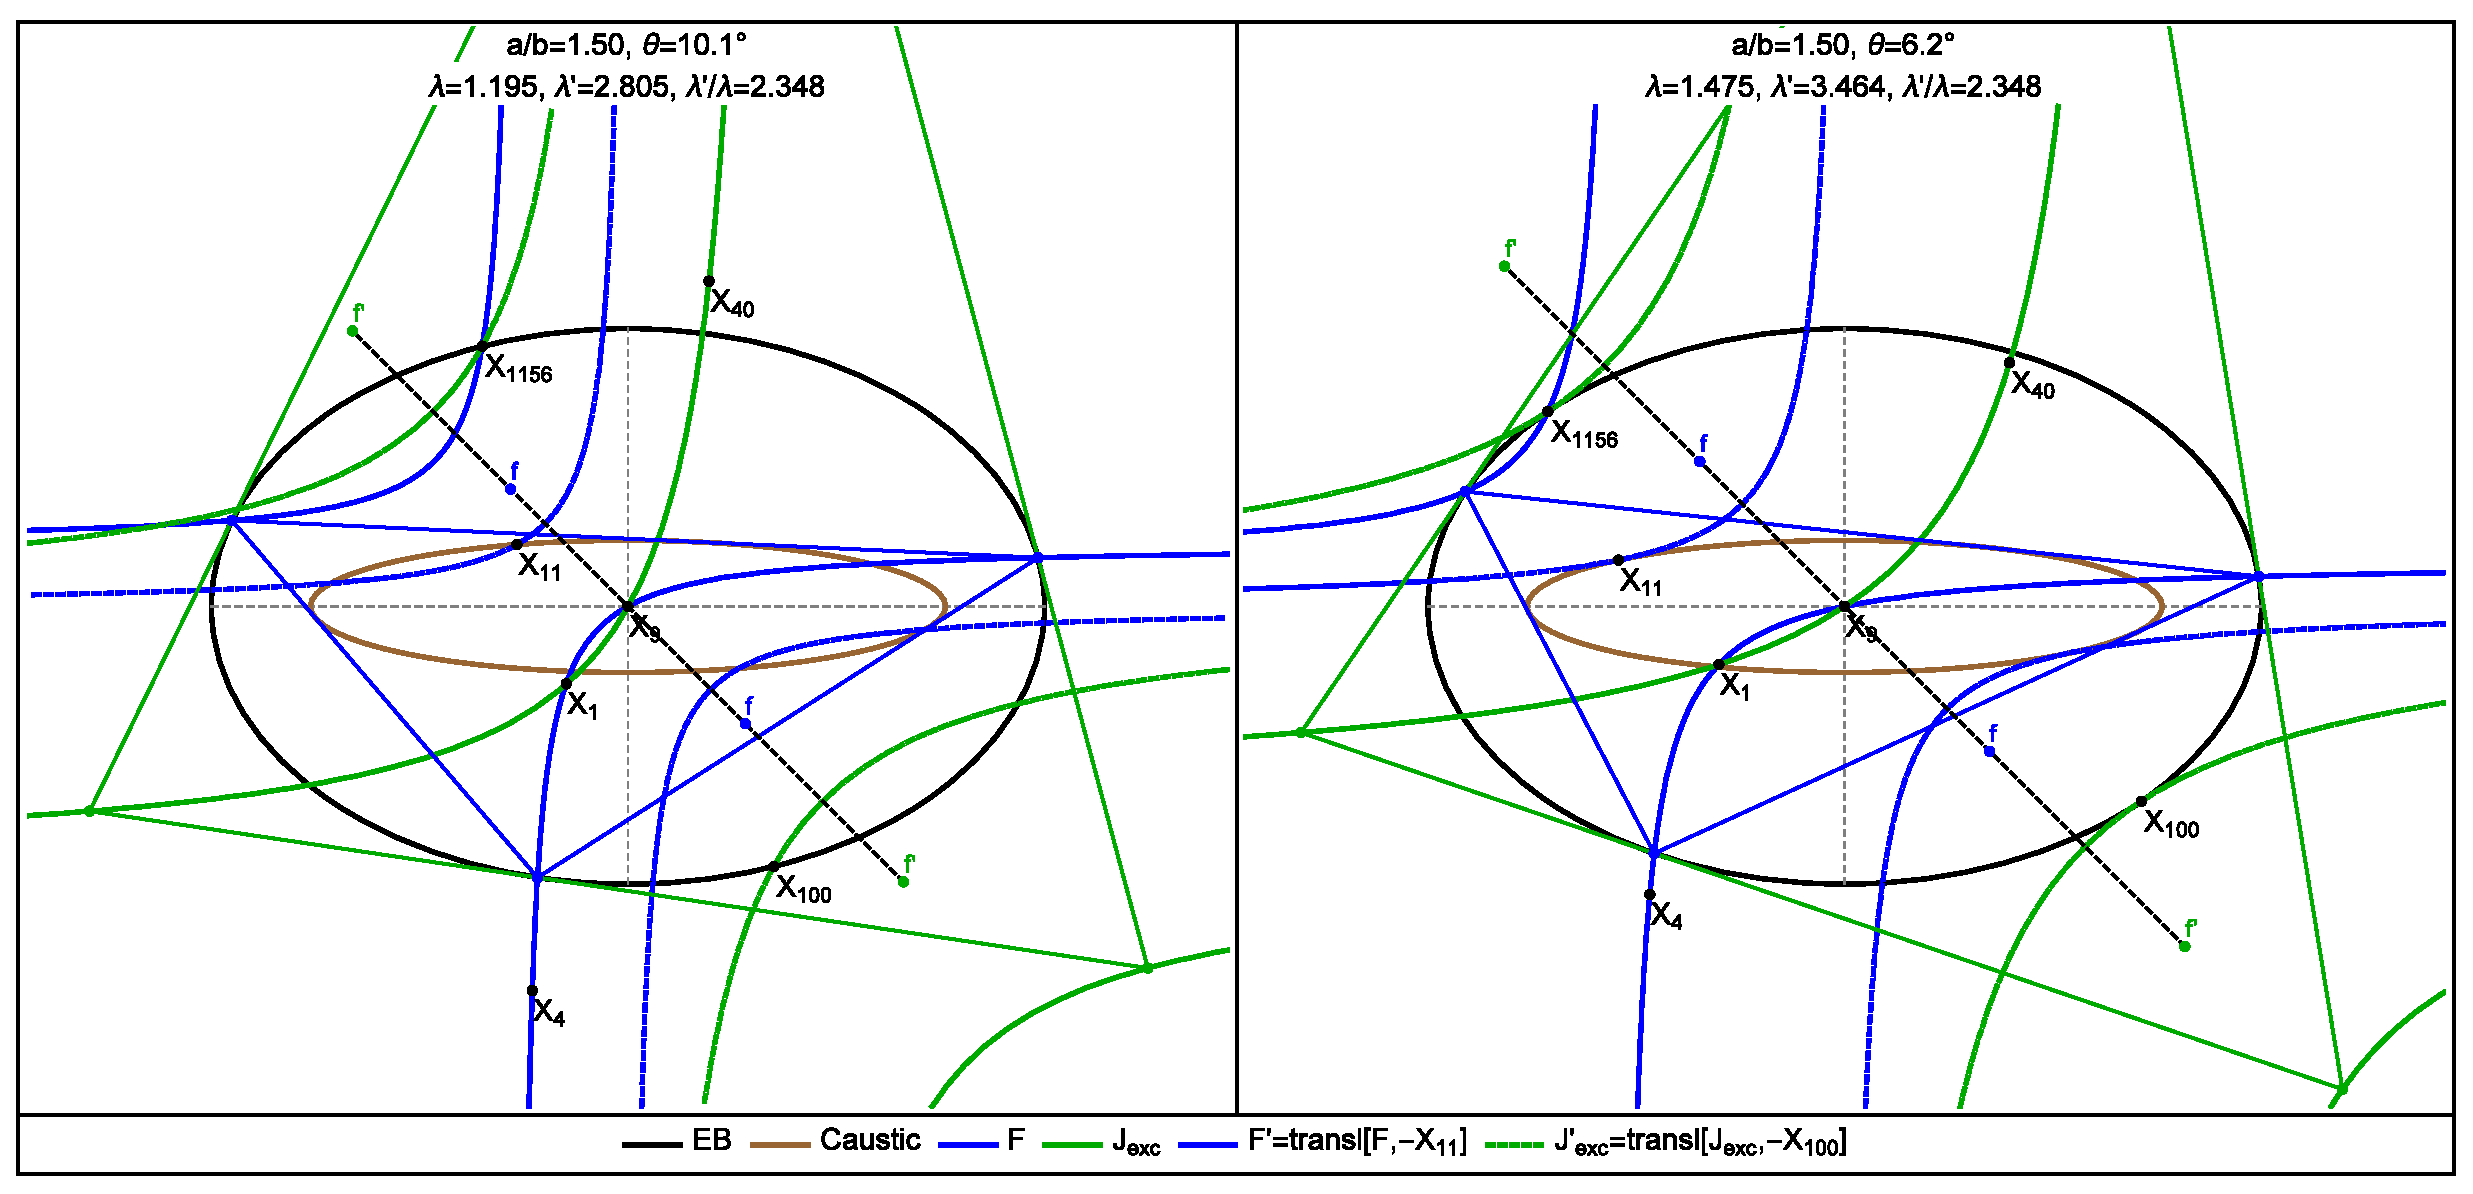
\includegraphics[width=\textwidth]{pics_eps_new/0100_zero_hyps.eps}
    \caption{Two snapshots of $J$ and $F_{exc}$ drawn solid blue and solid green, respectively, for $a/b=1.5$. Also shown (dashed) are copies $F'$ and $J'_{exc}$ of both hyperbolas translated so they are dynamically concentric with the EB (translate $J$ by $-X_{11}$ and $F_{exc}$ by $-X_{100}$). Their focal lengths $\lambda,\lambda'$ are identical to the original ones; their focal axes are collinear and shown the dashed diagonal through the EB center. Notice that like $F$, $J'$ also intersects the EB at $X_{1156}$. \textbf{Left}: $t=10.1^\circ$, showing an intermediate value of ether focal length. \textbf{Right}: $t=6.2^\circ$, focal lengths are at a maximum. When this happens, the translated copy of $F$ (resp. $J_{exc}$) is tangent to the Caustic (resp. EB) at $X_{11}$ (resp. $X_{1156})$. \textbf{Video}: \cite[PL\#09,10]{reznik2020-playlist-circum}}
    \label{fig:zero-hyps}
\end{figure}

\

%\section{Pythagorean Circumbilliards}
%\label{sec:pythagorean}
%We have seen \cite{ronaldo2020-loci} that with $a/b>a_4=\sqrt{2\,\sqrt{2}-1}\simeq{1.352}$ the orbit family contains obtuse triangles amongst which there always are 4 right triangles (identical up to rotation and reflection). An interesting question is which EB aspect ratios produce primitive {\em Pythagorean} triangles, i.e., right triangles with sides $s_1,s_2,s_3$ for which $s_1,s_2$ are co-prime, and $s_3^2=s_1^2+s_2^2$.

Start with an elementary Pythagorean triangle $P_1=(0,0)$, $P_2=(s_1,0)$, and $P_3=(s_1,s_2)$ choosing $s_1,s_2$ integers such that $s_3=s_3=\sqrt{s_1^2+s_2^2}$ is an integer.
The Circumbilliard is given by
\[
E_9(x,y)= s_2 x^2+ \left( s_3-s_1-s_2 \right) xy+s_1{y}^{2}-s_1s_2x-s_1 \left( s_1-s_3 \right) y=0.\]

Computing the axes of its Circumbilliard we obtain: 

\begin{equation}
    [a/b](s_1,s_2,s_3)= \frac {s_1+s_2+\sqrt {s_3\left(3\,s_3-2\,s_1-2\,s_2\right) }}{\sqrt { \left( 
s_1+s_2+3\,s_3 \right)  \left( s_1+s_2-s_3 \right) }}
\end{equation}

%\begin{equation*}
  %  \lim_{s_2\to \infty} %r(s_2,s_2,\sqrt{2}s_2)=\sqrt{2\sqrt{2}-1}\simeq %1.352
%\end{equation*}
%The axis of the Circumbilliard are:

%\begin{align}
%    a(m,n,p)=&  \\
 %   b(m,n,p)=&
%\end{align}

Table~\ref{tab:pythagorean} shows the aspect ratios required for the first 16 Pythagorean triples ordered by hypotenuse\footnote{The $a/b$ which produces $3:4:5$ was first computed in \cite{ronaldo2020-loci} in connection with $X_{88}$.}

\begin{table}[H]
\scriptsize
$$
\begin{array}{r|c|l|l}
(s_1,s_2,s_3) & a/b & {\simeq}a/b & \text{isosc. rank} \\
\hline
3, 4, 5 & {(7+\sqrt{5})\sqrt{11}}/{22} &  1.392 &  4 \\
5, 12, 13 & {\sqrt{14} (\sqrt{65}+17)}/{56} & 1.674 &  10 \\
8, 15, 17 & {\sqrt{111} (\sqrt{85}+23)}/{222} & 1.529 & 8\\
7, 24, 25  & {\sqrt{159} (5\,\sqrt{13}+31)}/{318} & 1.944 & 12 \\
\mathbf{20, 21, 29} & \mathbf{\sqrt{6} (\sqrt{145}+41)/{96}} & \mathbf{1.353} &  \mathbf{1} \\
12, 35, 37 & {\sqrt{395} (\sqrt{629}+47)}/{790} & 1.813 & 11 \\
9, 40, 41 & {\sqrt{86} (5\,\sqrt{41}+49)}/{344}& 2.184 &  14 \\
28, 45, 53 & {\sqrt{290} (\sqrt{689}+73)}/{1160} & 1.457 & 5 \\
11, 60, 61 & {\sqrt{635} (\sqrt{2501}+71)}/{1270} & 2.401 & 15 \\
16, 63, 65 & {\sqrt{959} (\sqrt{2405}+79)}/{1918} & 2.067 & 13 \\
33, 56, 65 & {\sqrt{426} (\sqrt{1105}+89)}/{1704} & 1.481  & 6 \\
48, 55, 73 & {\sqrt{2415} (\sqrt{949}+103)}/{4830} & 1.361 &  3 \\
\mathbf{13, 84, 85} & \mathbf{\sqrt{66} (97+\sqrt{5185})/{528}} & \mathbf{2.600} & \mathbf{16} \\
36, 77, 85 & {\sqrt{161} (\sqrt{2465}+113)}/{1288} & 1.602 & 9 \\
39, 80, 89 & {\sqrt{2895} (\sqrt{2581}+119)}/{5790} & 1.578 &  8 \\
65, 72, 97 & {\sqrt{1070} (\sqrt{1649}+137)}/{4280}& 1.357 & 2
\end{array}
$$
%\[a/b_{\perp}(m,n,p)=\sqrt {{\frac {m+n+\sqrt {p %( -2\,m-2\,n+3\,p \right) }}{m+n-
%\sqrt {p ( -2\,m-2\,n+3\,p \right) }}}}\]
\caption{The first column shows the first 16 Pythagorean triples ordered by hypotenuse $s_3$. The second one shows the $a/b$ family which produces it. The boldfaced triple $(20,21,29)$ (resp.~$(13,84,85)$) is the closest (resp.~farthest) to an isosceles in the table. This means $a/b$ will be closest to $a_4=1.352$. If rows were listed in ascending order of  $|s_1/s_2-1|$ (how scalene a triple is), the values of $a/b$ would also appear ascending, as indicated by the ``rank'' column.}
\label{tab:pythagorean}
\end{table}
%


\subsection{First 12k Pythagoreans in $a,b$ space}

Euclid's Algorithm generates a primitive Pythagorean triple from a co-prime pair $m,n$, $m>n$. For example, $(3,4,5)$ (resp.~$(5,12,13)$) is generated with $m=2,n=1$ (resp., $m=3,n=2$), etc.

Figure~\ref{fig:pythagorean} shows the first 12231 triangles generated in this fashion with $1<m<200$ in both $(s_1,s_2)$ and $(a,b)$ space. A few interesting observations are given in the caption. 

\begin{figure}[H]
    \centering
    \includegraphics[width=\textwidth]{pics_eps/0101_pythagorean_legs_ab.eps}
    \caption{\textbf{Top}: Right-triangles generated by Euclid's Algorithm with $n<m<200$, $m,n$ co-prime. Roughly 12k $(s_1,s_2)$ leg combinations are shown as black dots. To save space, the y-axis is drawn half-scale and points with $s_2>50000$ are not drawn. The green line represents $s_1=s_2$, i.e., isosceles triangles (only quasi-isosceles can be generated). The red (resp.~blue) curve is drawn over triangles obtained with $m=150$ (resp.~$n=150$). \textbf{Bottom}: Axes $(a,b)$ combinations which can produce the aforementioned right-triangles. The point cloud is properly under the green line $a/b=a_4$ (aspect ratio which produces an isosceles right-triangle). The constant $m=150$ (resp.~$n=150$) runs produce a red (resp.~blue) arch in $(a,b)$ space. Quasi-similar triangles organize in straight lines from the origin toward the right, i.e., they are generated by quasi-similar billiards.}
    \label{fig:pythagorean}
\end{figure}

\subsection{Iso-perimetric Primitive Pythagoreans}

Out of the 12231 Pythagorean triples generated, only 11548 perimeters $s_1+s_2+s_3$ are unique. Out of these, 10912 are associated with a single triple. An additional 585 (resp.~47) unique perimeters are each produced by two (resp.~3) distinct triples. Finally, 2 unique perimeters -- 60060 and 78540 -- are shared by two distinct groups of four triples, listed below:

$$
\scriptsize
\begin{array}{|c|c|c|c|}
\hline
\text{L} & s_1 & s_2 & s_3 \\
\hline
 60060 & 6699 & 26260 & 27101 \\
 60060 & 15960 & 19162 & 24938 \\
 60060 & 22035 & 12628 & 25397 \\
 60060 & 26936 & 5610 & 27514 \\
 78540 & 13515 & 31108 & 33917 \\
 78540 & 21896 & 24090 & 32554 \\
 78540 & 25179 & 20740 & 32621 \\
 78540 & 34440 & 8602 & 35498 \\
 \hline
\end{array}
$$

The perimeter $L$ of a 3-periodic orbit as a function of the EB axes $a,b$ is given by \cite{ronaldo2020-loci}:

\begin{equation*}
L=\frac{2(\delta+a^2+b^2)\sqrt{2\delta-a^2-b^2}}{a^2-b^2}
\end{equation*}

\noindent with $\delta=\sqrt(a^4-a^2 b^2+b^4)$. Each $L$ defines a level curve in $(a,b)$ space\footnote{Given by the quartic $(a^2-b^2)^2 L^4-(2(2a^2-b^2))(a^2-2 b^2)(a^2+b^2) L^2-27 a^4 b^4=0$.} which represents a 1d family of EBs such that all their orbit families have the same perimeter, see Figure~\ref{fig:iso-perimeter-3-and-4}.

The two groups of 4 triples with the same perimeter are shown in Figure~\ref{fig:iso-perimeter-4} against level curves of their perimeter. A similar picture for the 4-groups and 3-groups is shown in Figure~\ref{fig:iso-perimeter-3-and-4}.

\begin{figure}[H]
    \centering
    \includegraphics[width=.66\textwidth]{pics_eps/0120_fourTriplesPlot.eps}
    \caption{Two iso-perimetric curves are shown in $(a,b)$ space corresponding to EB families whose orbits have the same perimeter. Also shown are the 4-member groups of primitive Pythagorean triples sharing either perimeter.}
    \label{fig:iso-perimeter-4}
\end{figure}

\begin{figure}[H]
    \centering
    \includegraphics[width=.66\textwidth]{pics_eps/0121_fourTriplesAllPlot}
    \caption{All 4- and 3-groups of Pythagorean triples with the same perimeter. They fall on common iso-perimeter level curves (red) in $(a,b)$ space.}
    \label{fig:iso-perimeter-3-and-4}
\end{figure}

\section{Inconic Invariants}
\label{sec:inconic}
A triangle's {\em Inconic} touches its three sides while satisfying two other constraints, e.g., the location of its center. Similar to Circumconics, if the latter is interior to the 4 shaded regions in  Figure~\ref{fig:midlines} it is an ellipse, else it is a hyperbola. Lines drawn from each vertex to the Inconic tangency points concur at the perspector or Brianchon Point $B$ \cite{mw}.

Let the Inconic center $C$ be specified by Barycentrics\footnote{Barycentrics $g$ can be easily converted to Trilinears $f$ via: $f(s_1,s_2,s_3)=g(s_1,s_2,s_3)/s_1$ (cyclic) \cite{yiu2003}.} $g(s_1,s_2,s_3)$ (cyclic), then $B$ is given by $1/[g(s_2,s_3,s_1)+g(s_3,s_1,s_2)-g(s_1,s_2,s_3)]$ (cyclic) \cite{stothers2001-circumconics}. For example, consider the Inconic centered on $X_1$ (the Incircle), i.e., $g=s_2 s_3$ (cyclic). Then $B=1/(s_1 s_3+s_1 s_2-s_2 s_3)$. Dividing by the product ${s_1}{s_2}{s_3}$ obtain $B=1/(s_2 + s_3 - s_1)$ (cyclic), confirming that the perspector of the Incircle is the Gergonne Point $X_7$ \cite[Perspector]{mw}. The contact points are the vertices of the Cevian triangle through $B$.

Above we identified the confocal Caustic with the Mandart Inellipse $I_9$ \cite{mw} of the 3-periodic family, i.e., it is a stationary ellipse centered on $X_9$ and axis-aligned with the EB, Figure~\ref{fig:three-orbits-proof}. Its semi-axes $a_c,b_c$ are given by \cite{garcia2019-incenter}:

\begin{equation*}
a_c=\frac{a\left(\delta-{b}^{2}\right)}{a^2-b^2},\;\;\;
b_c=\frac{b\left({a}^{2}-\delta\right)}{a^2-b^2}\cdot
\end{equation*}

Similarly, the $X_9$-centered Inconic of the family of Excentral Triangles is the stationary EB, i.e., the EB is the Orthic Inconic \cite{mw} of the Excentrals.

\subsection{Excentral X$_3$-Centered Inconic}

No particular invariants have yet been found for any of the Inconics to 3-periodics with centers in $X_i$, $i=3,4,\ldots,12$. Let $I_3$ denote the $X_3$-centered inconic. Its Brianchon Point is $X_{69}$ and its foci aren't named centers \cite{moses2020-private-circumconic}.

\begin{remark}
$I_3$ is always an ellipse.
\end{remark}

To see this consider the Circumcenter of an acute, right, or obtuse triangle lies inside, on a vertex, or opposite to the interior of the Medial, respectively, i.e., within one of the 4 shaded regions in Figure~\ref{fig:midlines}.

Let $I'_3$ denote the $X_3$-centered Inconic of the Excentral Triangle. Its Brianchon Point is $X_{69}$ of the Excentral, i.e., $X_{2951}$ of the reference 3-periodic \cite{moses2020-private-circumconic}, Figure~\ref{fig:macbeath-excentral}(left).

\begin{remark}
$I'_3$ is axis-aligned with the EB and intersects it at $X_{100}$.
\end{remark}

\noindent Let $\mu'_3,\mu_3$ denote $I_3'$ major and minor semi-axes.

\begin{conjecture}
$\mu_3'/\mu_3$ is invariant over all 3-periodics and given by:

\begin{equation*}
\frac{\mu_3'}{\mu_3}=
%\frac{\sqrt{2\delta(\delta+ a^2 - b^2) - a^2 b^2}}{b^2} =
\frac{R+d}{R-d} = \frac{1+\sqrt{1-2\rho}}{\rho}-1
\end{equation*}
\label{conj:excIncX3}
\end{conjecture}

\noindent with $d=\sqrt{R(R-2r)}$, and $\rho=r/R$. The above has been derived for an isosceles 3-periodic. It matches the ratio numerically for any combination of $a,b$.

\subsection{Excentral  X$_5$-Centered (MacBeath) Inconic}

Above the locus of the Excenters is identified with the Excentral MacBeath Circumconic $E_6' $. The MacBeath {\em Inconic} $I_5$ of a triangle is centered on $X_5$ and has foci on $X_4$ and $X_3$. Its Brianchon Point is $X_{264}$, and it can be both an ellipse or a hyperbola \cite[MacBeath Inconic]{mw}. No invariants have yet been found for $I_5$.

Consider $I'_5$, the MacBeath Inconic of the Excentral Triangle, Figure~\ref{fig:macbeath-excentral}(right). The center and foci of $I'_5$ with respect to the reference triangle are $X_3$, $X_1$, and $X_{40}$, respectively, and its Brianchon is $X_{1742}$ \cite{moses2020-private-circumconic}. Unlike $I'_3$, the axes of $I'_5$ are askew with respect to the EB.

\begin{remark}
$I'_5$ is always an ellipse.
\end{remark}

This is due to the fact that the Excentral is acute as is its homothetic Medial. Since $X_5$ is the latter's Circumcenter, it must lie inside it.

\noindent Let $\mu'_5,\mu_5$ denote $I_5'$ major and minor semi-axes.

\begin{conjecture}
$\mu_5'/\mu_5$ is invariant over all 3-periodics and given by:

\begin{align*}
 \frac{\mu'_5}{\mu_5} =
 %\frac {\left( {b}^{2}+\delta \right) \sqrt {\delta+{a}^{2}-{b}^{2} } }{2b{a}^{2}}=
 %\frac {\left( {a}^{2}+\delta \right) \sqrt {\delta+{b}^{2}-{a}^{2}} }{2a{b}^{2}} =
\frac{R}{\sqrt{R^2-d^2}}=\frac{1}{\sqrt{2 \rho}}
\end{align*}
\label{conj:excIncX5}
\end{conjecture}

The above was derived for an isosceles 3-periodic and shown to work for any $a,b$.

\begin{figure}
    \centering
    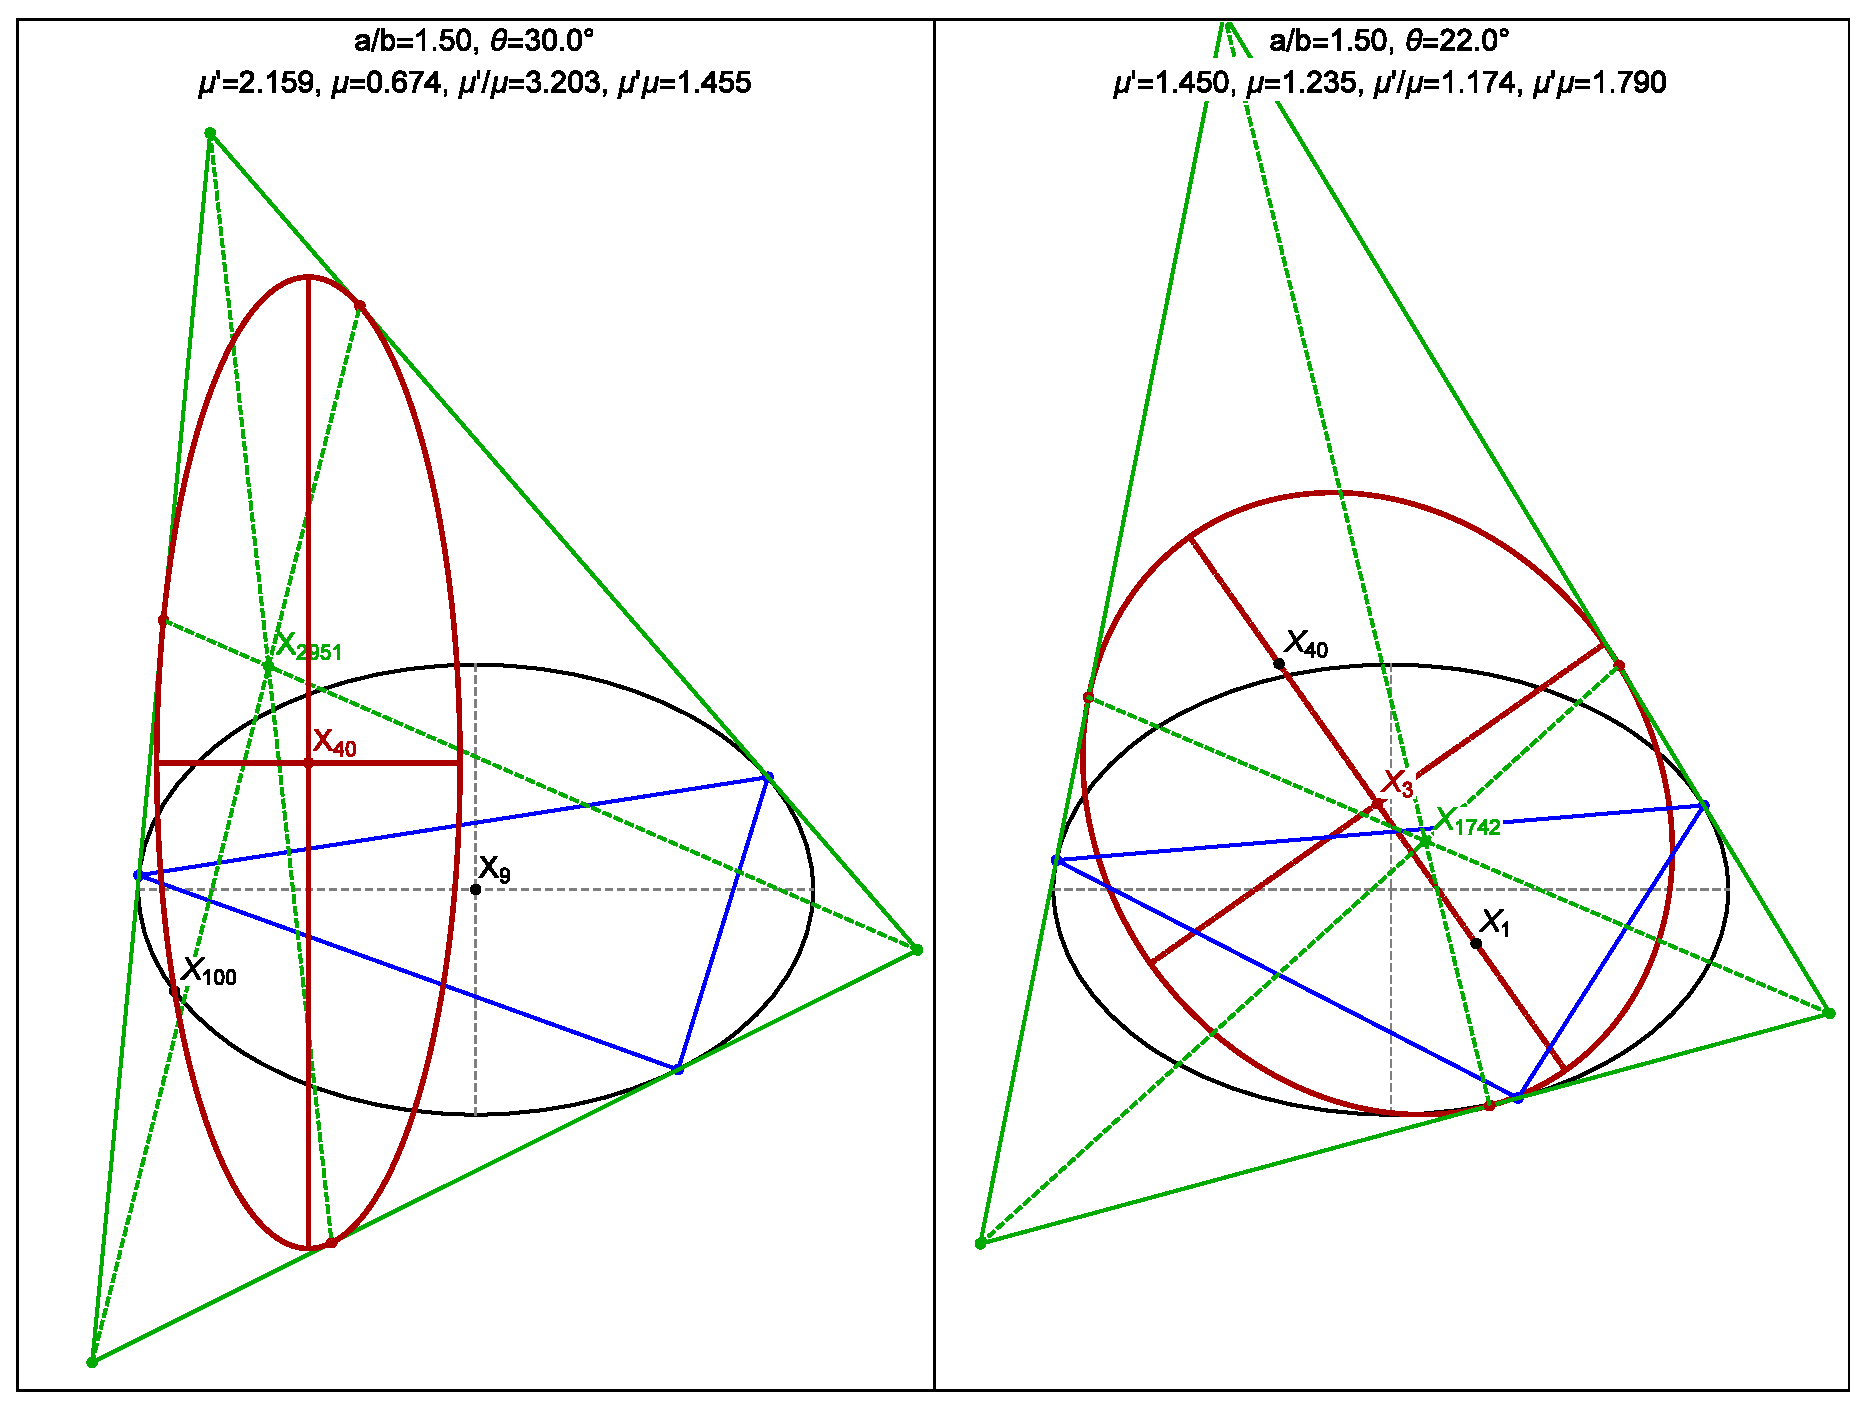
\includegraphics[width=\textwidth]{pics_eps_new/0150_two_inconics.eps}
    \caption{\textbf{Left}: The $X_{3}$-centered Inconic (red) of the Excentral Triangle (green), whose center is $X_{40}$ in terms of the 3-periodic (blue). Its Brianchon Point is $X_{2951}$ \cite{moses2020-private-circumconic}. This Inconic's axes are aligned with the EB which it intersects at $X_{100}$, and its aspect ratio is invariant. \textbf{Right}: The MacBeath Inconic of the Excentral (red) is centered on the latter's $X_5$ and has foci on $X_4$ and $X_3$. These correspond to  $X_3$, $X_1$, and $X_{40}$ of the reference triangle (blue). Its Brianchon Point is $X_{1742}$ \cite{moses2020-private-circumconic}. Though its axes are askew with respect to the EB, its aspect ratio is invariant over the 3-periodic family. \textbf{Video}: \cite[PL\#11]{reznik2020-playlist-circum}.}
    \label{fig:macbeath-excentral}
\end{figure}

\section{Conclusion}
\label{sec:conclusion}
Videos mentioned above have been placed on a \href{https://bit.ly/379mk1I}{playlist} \cite{reznik2020-playlist-circum}. Table~\ref{tab:playlist} contains quick-reference links to all videos mentioned, with column ``PL\#'' providing video number within the playlist.

Additionally to Conjecture~\ref{conj:moses} we submit the following questions to the reader:

\begin{itemize}
  \item Can alternate proofs be found for Theorems~\ref{thm:axis-ratio} and \ref{thm:focal-ratio} with tools of algebraic and/or projective geometry?
  \item Are there other notable circumconic pairs which exhibit interesting invariants?
  \item Can any of the invariants cited above be generalized to $N$-periodics?
  \item Can the invariant aspect ratios for the Excentral Inconics mentioned in Section~\ref{sec:inconic} be proven?
    \item Are there other Inconic invariants over 3-periodics and/or their derived triangles? 
    \item Are there interesting properties for the loci of the {\em foci} of Feuerbach and/or Jerabek Circumhyperbolas?
    \item The Yff Circumparabola whose focus is on $X_{190}$ is shown in \cite[PL\#12]{reznik2020-playlist-circum} over 3-periodics. Are there interesting invariants?
    \item Does any Triangle Circumcubic display interesting invariants over 3-periodics? We found none for the Thomson Cubic shown in \cite[PL\#13]{reznik2020-playlist-circum}. How about the Darboux, Neuberg, Lucas, and myriad others catalogued in \cite{gibert2020-cubics}.
    \item The ratio of focal lengths of $F$ by $J_{exc}$ is numerically invariant for the Poristic family. Can this be proved?
    \item Like 3-periodics, poristic triangles conserve $r/R$. Can a continuous map be specified between the two families? Are there any interesting properties?
\end{itemize}

\begin{table}
%\scriptsize
\begin{tabular}{c|l|l}
\href{https://bit.ly/2NOOIOX}{PL\#} & Title & Section\\
\hline

\href{https://youtu.be/tMrBqfRBYik}{01} &
{Mittenpunkt stationary at EB center} & \ref{sec:intro} \\

\href{https://youtu.be/vSCnorIJ2X8}{02} &
{Circumbilliards (CB) of Various Triangles} &
\ref{sec:cb} \\

\href{https://youtu.be/Og7xLgkrLqw}{03} &
{CBs of Derived Triangles and Loci of Centers} &
\ref{sec:cb_derived} \\

\href{https://youtu.be/xyHUwpvAj3g}{04} & CBs of ACT and Medial (separate) &
\ref{sec:cb_derived} \\

\href{https://youtu.be/e-mToZlkHtc}{05} &
CBs of ACT and Medial (superposed) & \ref{sec:cb_derived} \\

\href{https://youtu.be/5KL8st2vIb0}{06} &
{CB of Orthic and Locus of its Mittenpunkt} &
\ref{sec:cb_derived} \\

\href{https://youtu.be/yEu2aPiJwQo}{07} & \makecell[lt]{Invariant Aspect Ratio of \\Circumbilliard of Poristic Family} &
\ref{sec:cb_derived} \\

\href{https://youtu.be/P_Io7HsWGnQ}{08} &
{The $X_1$- and $X_2$-centered Circumellipses} &
\ref{sec:circumellipses} \\

\href{https://youtu.be/Pz4tUijYZCA}{09} &
\makecell[lt]{Orbit Feuerbach and \\ Excentral Jerabek Circumhyperbolas} &
\ref{sec:circumhyperbolae} \\

%\href{https://youtu.be/7Q1TCbW2jFM}{10} &
%Excentral CB and its Jerabek Hyperbola &
%\ref{sec:circumhyperbolae} \\

\href{https://youtu.be/ewioM6-nCpY}{10} &
Invariant Focal Length Ratio for $F$ and $J_{exc}$ &
\ref{sec:circumhyperbolae} \\

\href{https://youtu.be/CHbrZvx1I8w}{11} &
\makecell[lt]{
Excentral MacBeath and $X_3$-Centered\\Inconics: Invariant Aspect Ratio
} &
\ref{sec:inconic} \\

\href{https://youtu.be/Sm9g5lqhZbk}{12} & The Yff Circumparabola of 3-Periodics &
\ref{sec:conclusion} \\

\href{https://youtu.be/s-h72iorZKw}{13} & The Thomson Cubic of 3-Periodics &
\ref{sec:conclusion} \\

%\href{https://youtu.be/DS4ryndDK6Q}{15} & Invariants of the Poristic Triangle Family &
%\ref{sec:conclusion} \\

\end{tabular}
\caption{Videos mentioned in the paper. Column ``PL\#'' indicates the entry within the playlist \cite{reznik2020-playlist-circum}}
\label{tab:playlist}
\end{table}


\section*{Acknowledgments}
We would like to thank Peter Moses and Clark Kimberling for their prompt help with dozens of questions. A warm thanks goes out to Profs. Jair Koiller and Daniel Jaud who provided critical editorial help.

The second author is fellow of CNPq and coordinator of Project PRONEX/ CNPq/ FAPEG 2017 10 26 7000 508.

\bibliographystyle{alpha}
\bibliography{elliptic_billiards_v3,authors_rgk_v1} 
%\bibliography{test}

\appendix
\section{Triangle Centers}
\label{app:triangle-centers}
Kimberling's Encyclopedia of Triangle Centers (ETC) \cite{etc} describes constructions and properties for thousands of such Centers, identified as $X_i$: $X_1$ for Incenter, $X_2$ for Barycenter, etc. Trilinear and/or Barycentric Coordinates are also provided for each Center. The former are signed distances to the sides of a triangle $T=P_1P_2P_3$, i.e. they are invariant with respect to similarity/reflection transformations, see Figure~\ref{fig:trilins}.

\begin{figure}
    \centering
    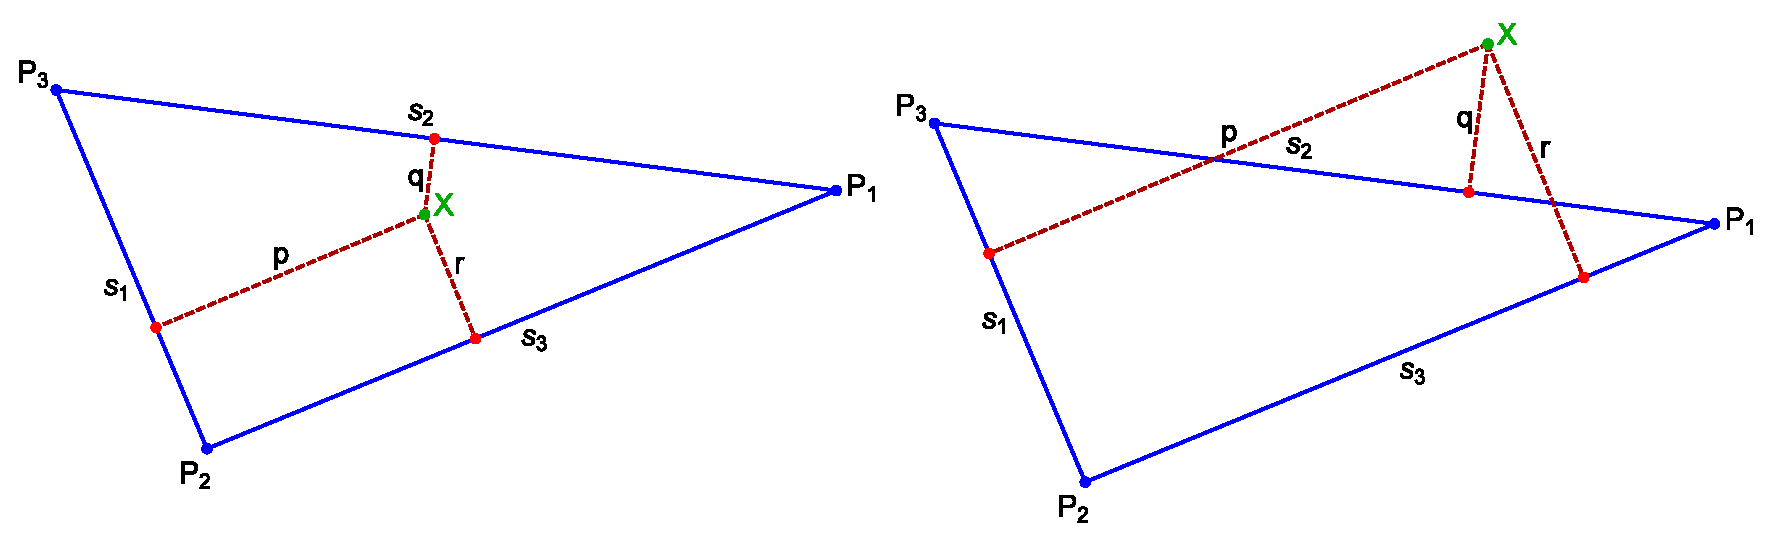
\includegraphics[width=\textwidth]{pics_1120_trilins.eps}
    \caption{Trilinear coordinates $p:q:r$ for a point $X$ on the plane of a generic triangle $T=P_1P_2P_3$ are homogeneous signed distances to each side whose lengths are $s_1,s_2,s_3$. The red dots are known as the {\em pedal points} of $X$ \cite{mw}. The left (resp. right) figure shows an interior (resp. exterior) point. In both cases $p,r$ are positive however $q$ is positive (resp. negative) in the former (resp. latter) case.}
    \label{fig:trilins}
\end{figure}

Trilinears can be easily converted to Cartesians using \cite{mw}:

\begin{equation}
\label{eqn:trilin-cartesian}
X=\frac{p s_1 P_1 + q s_2 P_2 + r s_3 P_3}{p{s_1}+q{s_2}+r{s_3}}
\end{equation}

\noindent where $s_1=|P_3-P_2|$, $s_2=|P_1-P_3|$ and $s_3=|P_2-P_1|$ are the sidelengths, Figure~\ref{fig:trilins}.
For instance, the Trilinears for the barycenter are $p = s_1^{-1},\,q = s_2^{-1},\,r = s_3^{-1}$, yielding the familiar $X_2 = (P_1+P_2+P_3)/3$.

%A point on the plane of a triangle $T=P_1P_2P_3$ can be defined by a triple $p:q:r$ of signed distances to each side\footnote{The Barycentrics of $p:q:r$ are $p\,s_1:q\,s_2:r\,s_3$ \cite{mw}.}, see Figure~\ref{fig:trilins}. This local coordinate system renders the point invariant under similarity transformations (rigid+dilation+reflection) of $T$.

A {\em Triangle Center} is such a triple obtained by applying a {\em Triangle Center Function} $h$ thrice to the sidelengths $s_1,s_2,s_3$ cyclically \cite{kimberling1993_rocky}:
 
\begin{equation}
\label{eqn:ftrilins}
    p:q:r {\iff} h(s_1,s_2,s_3):h(s_2,s_3,s_1):h(s_3,s_1,s_2)
\end{equation}

\noindent $h$ must (i) be {\em bi-symmetric}, i.e., $h(s_1,s_2,s_3)=h(s_1,s_3,s_2)$, and (ii) homogeneous, $h(t s_1, t s_2, t s_3)=t^n h(s_1,s_2,s_3)$ for some $n$ \cite{kimberling1993_rocky}.

Triangle Center Functions for a few Triangle Centers catalogued in \cite{mw} appears in Table~\ref{tab:center-trilinears}. Trilinears can be converted to Cartesians using \eqref{eqn:trilin-cartesian}.

\subsection{Constructions for Basic Triangle Centers}

Constructions for a few basic Triangle Centers are shown in Figure~\ref{fig:constructions}.

\begin{figure}
    \centering
    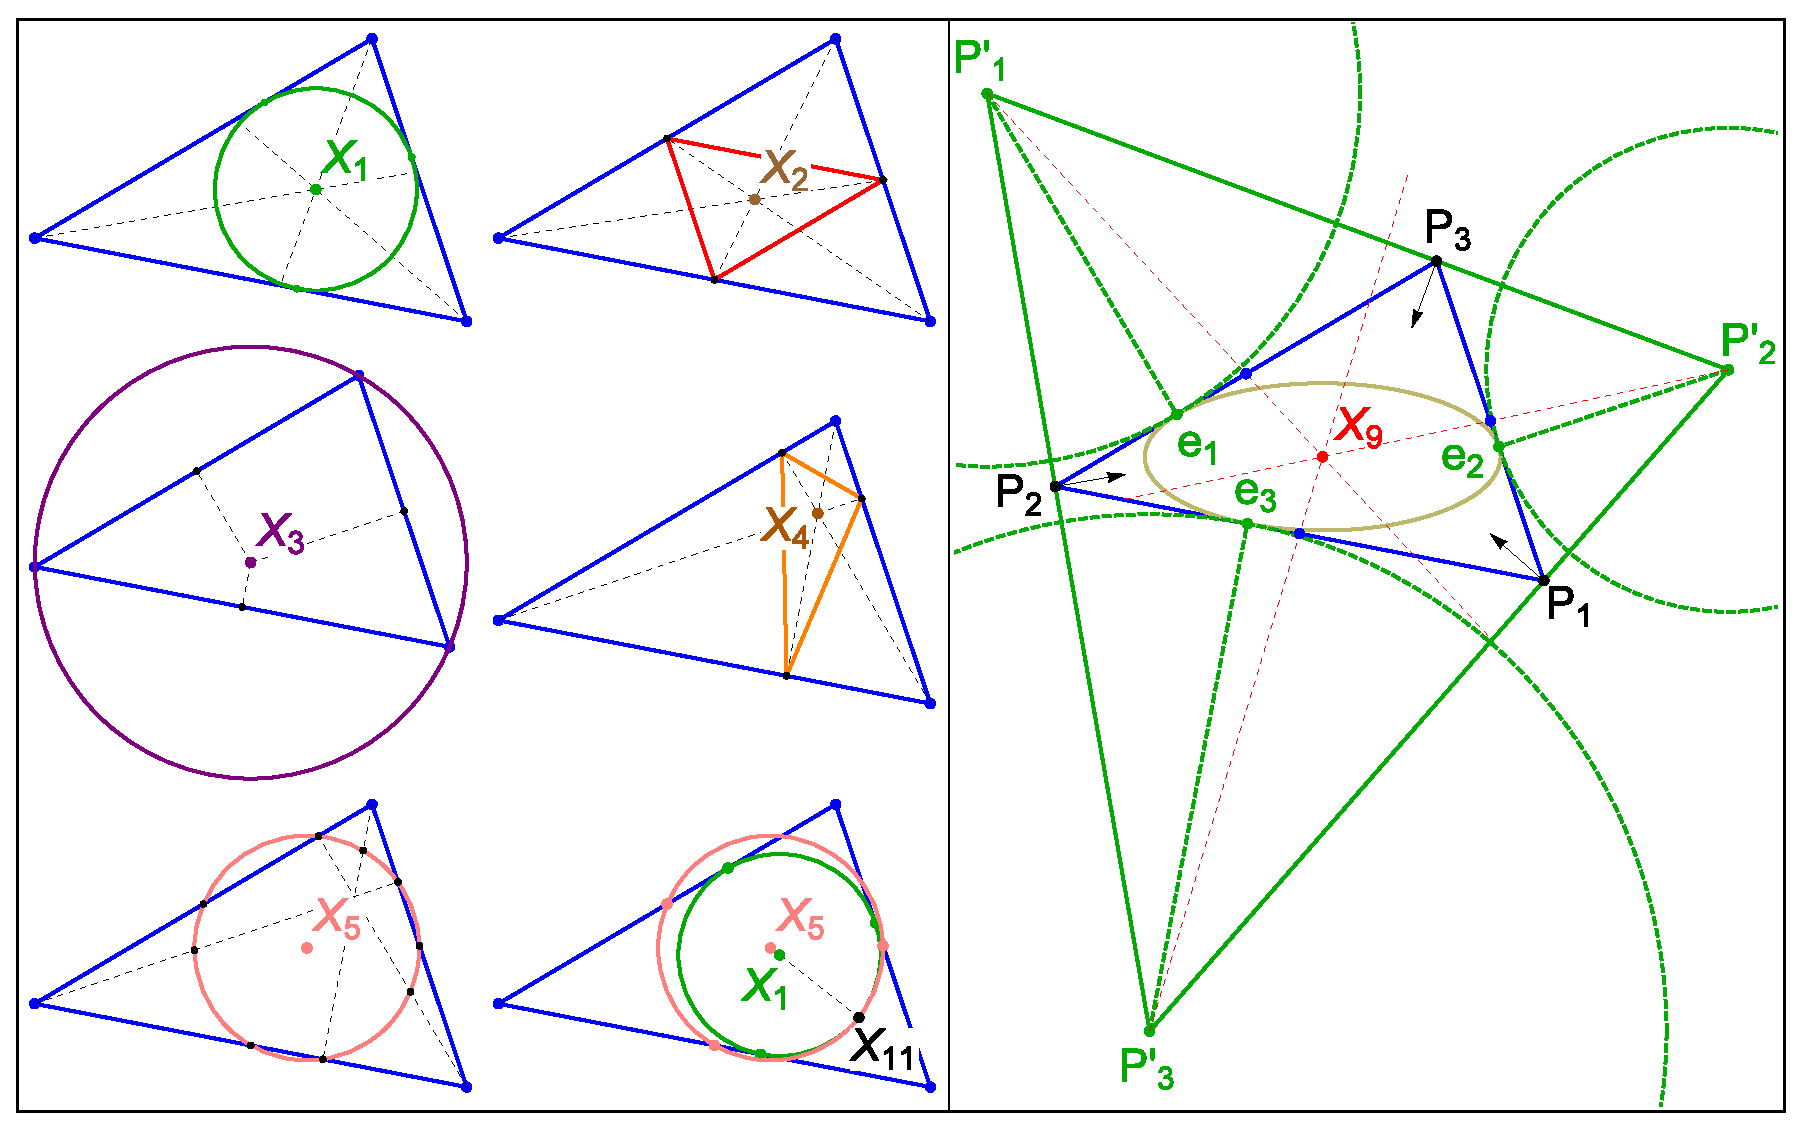
\includegraphics[width=\textwidth]{pics_1010_constr.eps}
    \caption{Constructions for Triangle Centers $X_i$, $i=1,2,3,4,5,9,11$, taken from \cite{reznik2020-intelligencer}.}
    \label{fig:constructions}
\end{figure}

\begin{itemize}
    \item The Incenter $X_1$ is the intersection of angular bisectors, and center of the Incircle (green), a circle tangent to the sides at three {\em Intouchpoints} (green dots), its radius is the {\em Inradius} $r$.
    \item The Barycenter $X_2$ is where lines drawn from the vertices to opposite sides' midpoints meet. Side midpoints define the {\em Medial Triangle} (red).
    \item The Circumcenter $X_3$ is the intersection of perpendicular bisectors, the center of the {\em Circumcircle} (purple) whose radius is the {\em Circumradius} $R$.
    \item The Orthocenter $X_4$ is where altitudes concur. Their feet define the {\em Orthic Triangle} (orange).
    \item $X_5$ is the center of the 9-Point (or Euler) Circle (pink): it passes through each side's midpoint, altitude feet, and Euler Points \cite{mw}.
    \item The Feuerbach Point $X_{11}$ is the single point of contact between the Incircle and the 9-Point Circle.
    \item Given a reference triangle $P_1P_2P_3$ (blue), the {\em Excenters} $P_1'P_2'P_3'$ are pairwise intersections of lines through the $P_i$ and perpendicular to the bisectors. This triad defines the {\em Excentral Triangle} (green).\
    \item The {\em Excircles} (dashed green) are centered on the Excenters and are touch each side at an {\em Extouch Point} $e_i,i=1,2,3$.
    \item Lines drawn from each Excenter through sides' midpoints (dashed red) concur at the {\em Mittenpunkt} $X_9$.
    \item Also shown (brown) is the triangle's {\em Mandart Inellipse}, internally tangent to each side at the $e_i$, and centered on $X_9$. This is identical to the $N=3$ Caustic.
\end{itemize}

\subsection{Derived Triangles}
\label{app:derived-tris}

A {\em Derived Triangle} $T'$ is constructed from the vertices of  a reference triangle $T$. A convenient representation is a 3x3 matrix, where each row, taken as Trilinears, is a vertex of $T'$. For example, the Excentral, Medial, and Intouch Triangles $T'_{exc}$, $T'_{med}$, and $T'_{int}$  are given by \cite{mw}: 

%, built from Triangle Center functions $h_1,h_2,h_3$ as follows \cite{kimberling1993_rocky}:

%\begin{align*}
%T'=
%\left[
%\begin{matrix}
%h_1(s_1,s_2,s_3) & h_2(s_1,s_2,s_3) & %h_3(s_1,s_2,s_3)\\ 
%   h_3(s_2,s_3,s_1) & h_1(s_2,s_3,s_1) & %h_2(s_2,s_3,s_1) \\
%   h_2(s_3,s_1,s_2) & h_3(s_3,s_1,s_2) & %h_1(s_3,s_1,s_2)
%\end{matrix}
%\right]
%\end{align*}

\begin{equation*}
\left[
\begin{matrix}
-1&1&1\\1&-1&1\\1&1&-1
\end{matrix}
\right],\;
\left[
\begin{matrix}
0&s_2^{-1}&s_3^{-1}\\s_1^{-1}&0&s_3^{-1}\\s_1^{-1}&s_2^{-1}&0
\end{matrix}
\right],\;
\left[
\begin{matrix}
0&\frac{s_1 s_3}{s_1-s_2+s_3}&\frac{s_1 s_2}{s_1+s_2-s_3}\\
\frac{s_2 s_3}{-s_1+s_2+s_3}&0&\frac{s_1 s_2}{s_1+s_2-s_3}\\
\frac{s_2 s_3}{-s_1+s_2+s_3}&\frac{s_1 s_3}{s_1-s_2+s_3}&0
\end{matrix}
\right]
\end{equation*}

A few Derived Triangles are shown in Figure~\ref{fig:derived-isosceles}, showing a property similar to Lemma~\ref{lem:axis-of-symmetry}, Appendix~\ref{app:method-lemmas}, namely, when the 3-periodic is an isosceles, one vertex of the Derived Triangle lies on the orbit's axis of symmetry.

\begin{figure}[H]
    \centering
    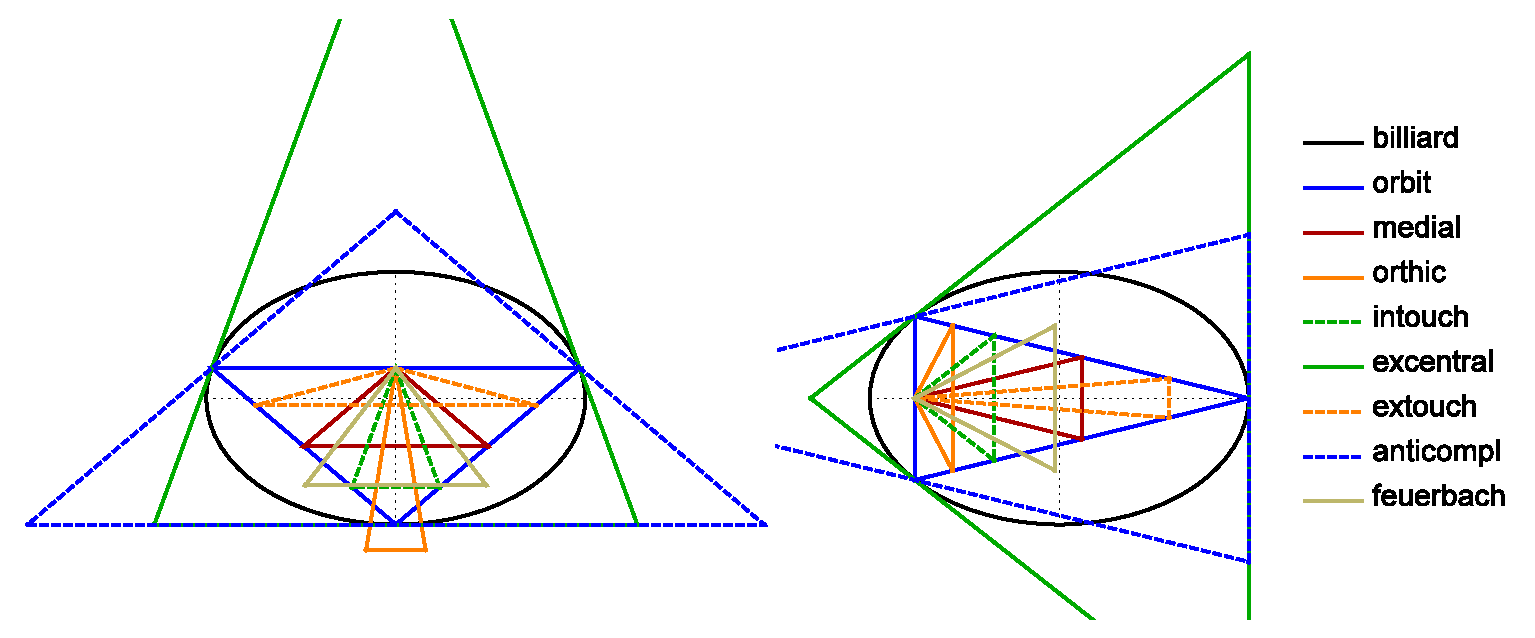
\includegraphics[width=\textwidth]{pics_1070_lemma3}
    \caption{When the orbit is an isosceles triangle (solid blue), any Derived Triangle will contain one vertex on the axis of symmetry of the orbit. \href{https://youtu.be/xyroRTEVNDc}{Video}}
    \label{fig:derived-isosceles}
\end{figure}





\section{Review: Elliptic Billiards}
\label{app:billiards}
An Elliptic Billiard (EB) is a particle moving with constant velocity in the interior of an ellipse, undergoing elastic collisions against its boundary \cite{rozikov2018,sergei91}, Figure~\ref{fig:billiard-trajectories}. For any boundary location, a given exit angle (e.g., measured from the normal) may give rise to either a quasi-periodic (never closes) or $N$-periodic trajectory \cite{sergei91}, where $N$ is the number of bounces before the particle returns to its starting location. All trajectory segments are tangent to a confocal Caustic \cite{sergei91}. The EB is a special case of {\em Poncelet's Porism} \cite{dragovic11}: if one $N$-periodic trajectory can be found departing from some boundary point, any other such point will initiate an $N$-periodic, i.e., a 1d {\em family} of such orbits will exist. A classic result is that $N$-periodics conserve perimeter \cite{sergei91}.

\begin{figure}
    \centering
    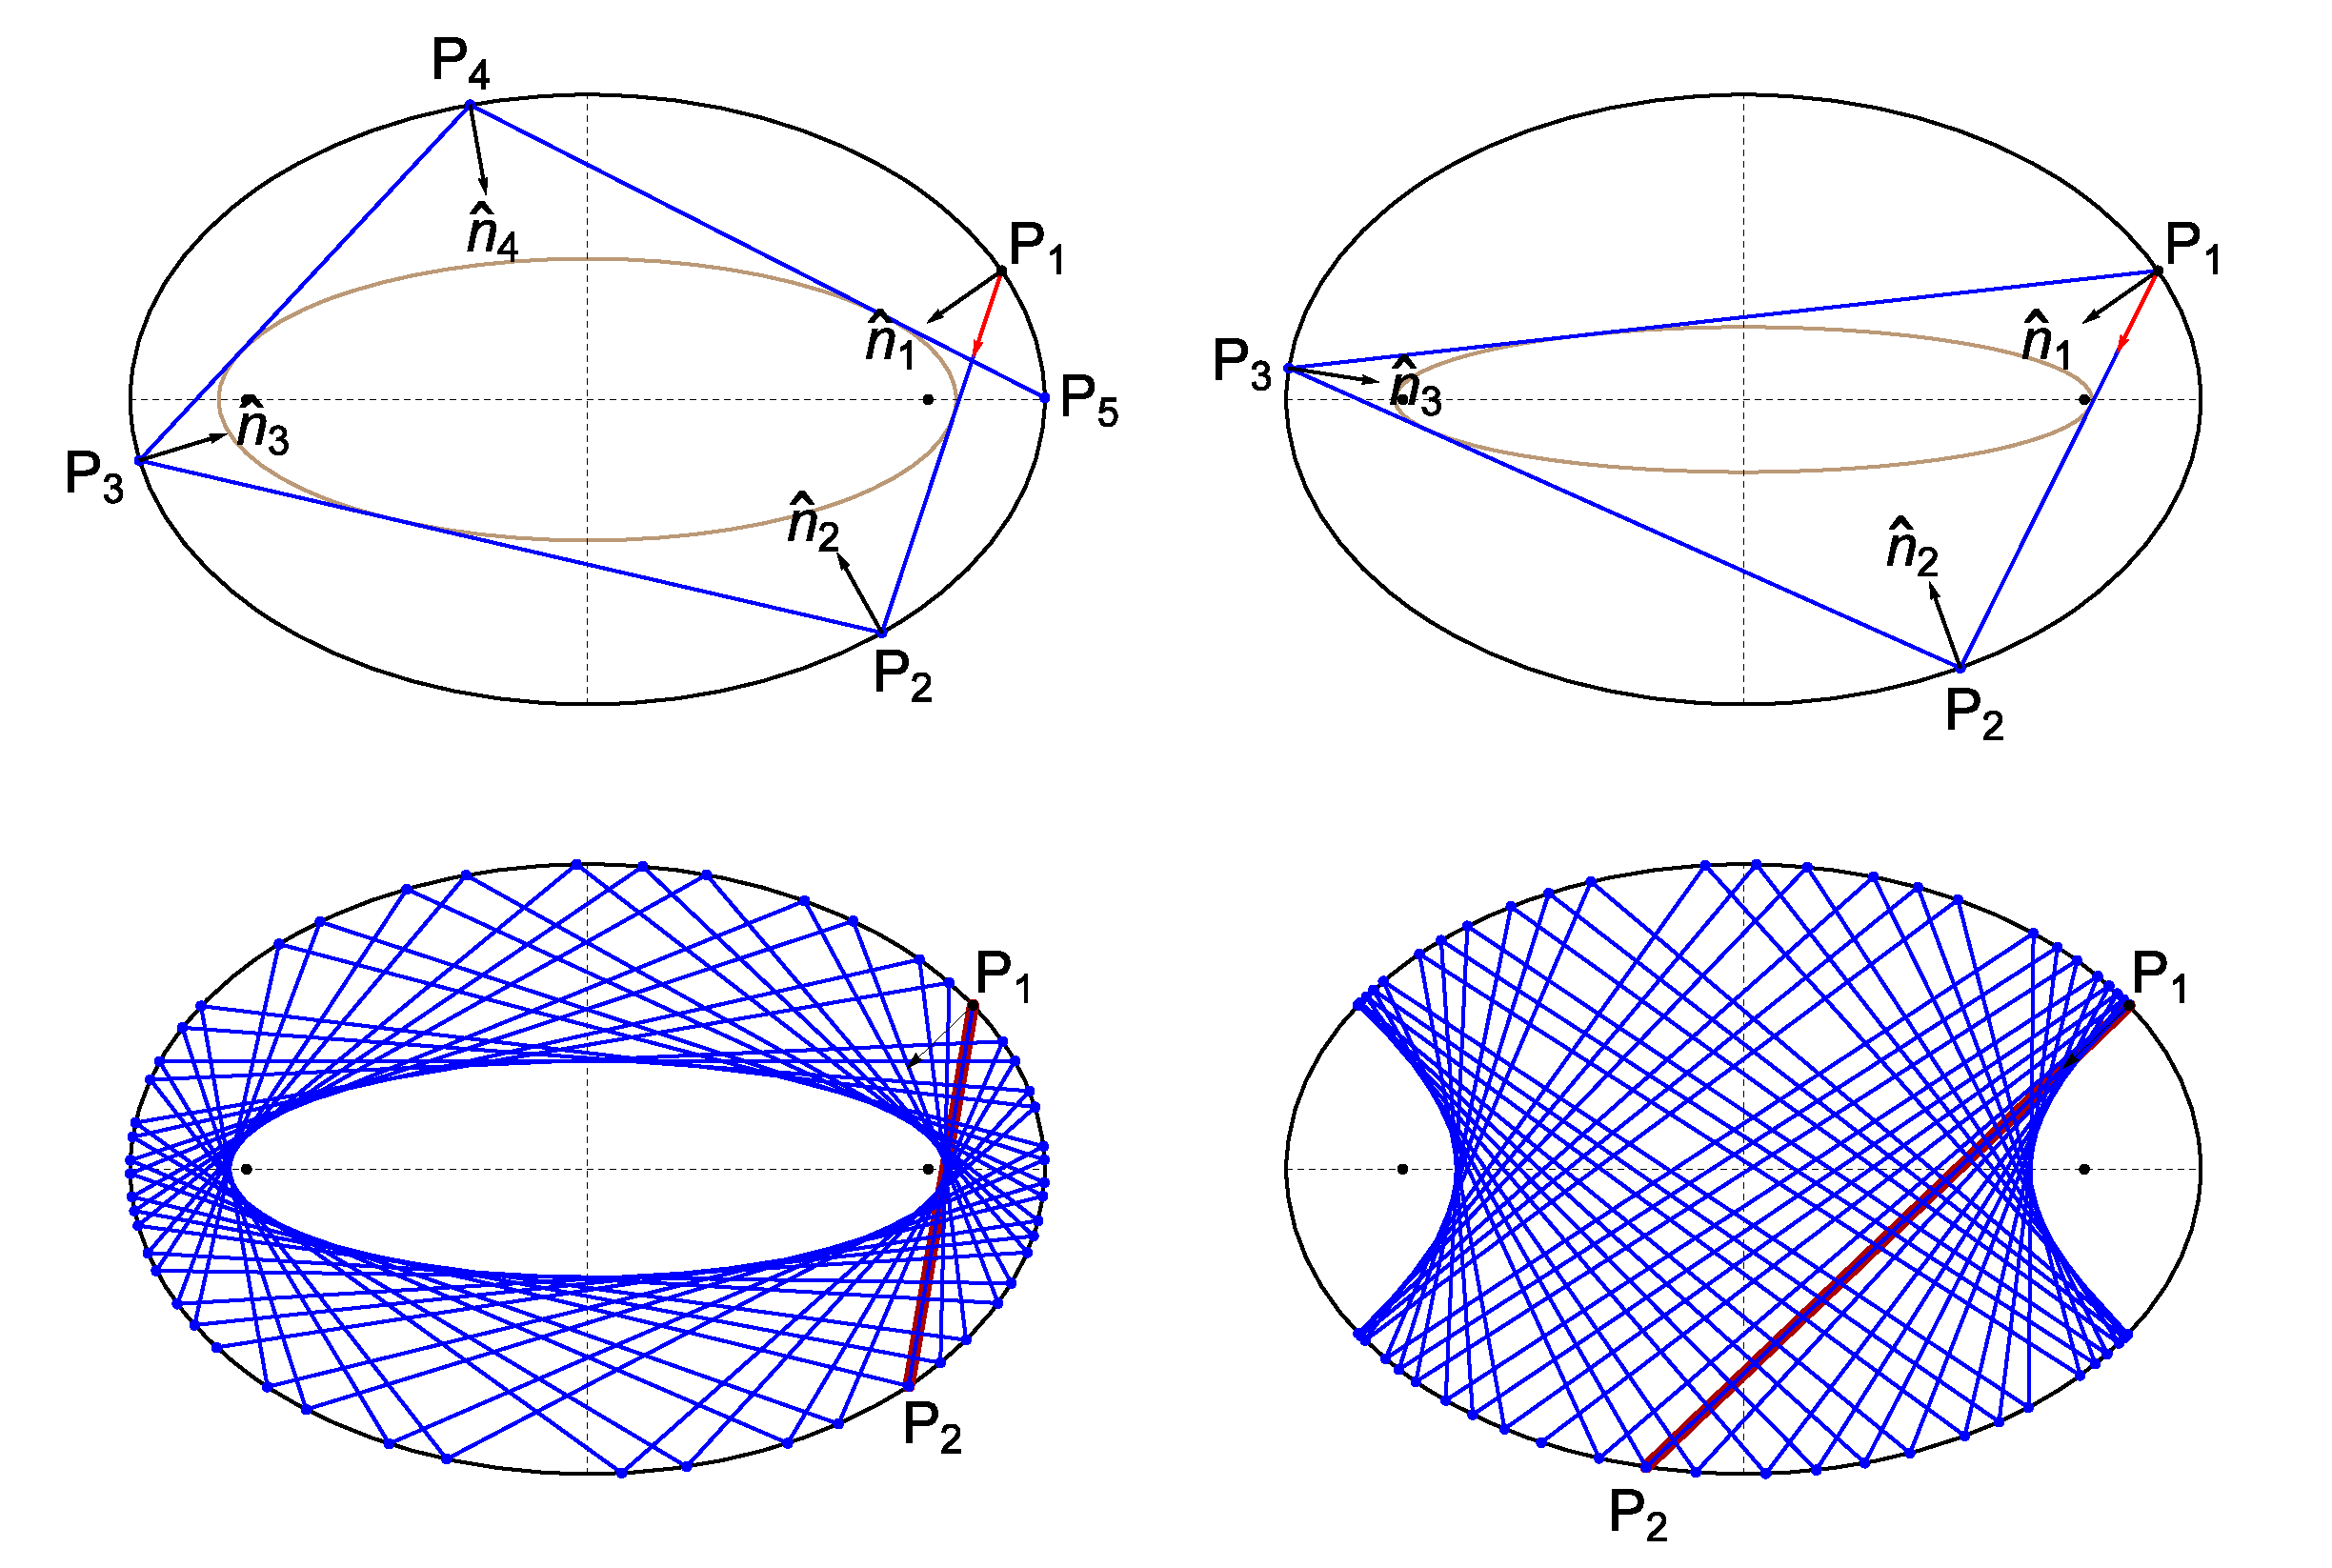
\includegraphics[width=\textwidth]{pics_1030_billiard_trajectories.eps}
    \caption{Trajectory regimes in an Elliptic Billiard, taken from \cite{reznik2020-intelligencer}. \textbf{Top left}: first four segments of a trajectory departing at $P_1$ and toward $P_2$, bouncing at $P_i, i=2,3,4$. At each bounce the normal $\hat{n}_i$ bisects incoming and outgoing segments. Joachimsthal's integral \cite{sergei91} means all segments are tangent to a confocal {\em Caustic} (brown). \textbf{Top right}: a 3-{\em periodic} trajectory. All 3-periodics in this Billiard will be tangent to a special confocal Caustic (brown). \textbf{Bottom}: first 50 segments of a non-periodic trajectory starting at $P_1$ and directed toward $P_2$. Segments are tangent to a confocal ellipse (left) or hyperbola (right). The former (resp. latter) occurs if $P_1P_2$ passes outside (resp. between) the EB's foci (black dots).}
    \label{fig:billiard-trajectories}
\end{figure}

\section{Expressions used in Section~\ref{sec:rational-trilinears}}
\label{app:rational-support}
Let the boundary of the Billiard satisfy Equation~\eqref{eqn:billiard-f}. Assume, without loss of generality, that $a{\geq}b$. Here we provide expressions used in Section~\ref{sec:algebraic}. Let $P_1,P_2,P_3$ be an orbit's vertices.

\subsection{Exit Angle Required for 3-Periodicity}
\label{app:exit-angle}

Consider a starting point $P_1=(x_1,y_1)$ on a Billiard with semi-axes $a,b$. The cosine of the exit angle $\alpha$ (measured with respect to the normal at $P_1$\footnote{i.e., $\alpha=\theta_1/2$.}) required for the trajectory to close after 3 bounces is given by \cite{garcia2019-incenter}: 

%\begin{equation}
%\label{eqn:cosalpha}
%\cos{\alpha}={\frac {a^2 b \, \sqrt {2 \delta-{a}^{2}-{b}^{2}}}{{c}^{2}\sqrt {{a}^{4}-{c}^{2} x_1^{2}}}}, \;\; c^2=a^2-b^2,\;\; \delta=\sqrt{a^4-a^2b^2+b^4}\,.
%\end{equation}
\begin{equation*}
\cos^2{\alpha}=\frac{d_1^2\delta_1^2}{\,d_2}=k_1,\;\;\;\sin{\alpha}\cos\alpha=\frac{ \delta_1d_1^2}{d_2 }\sqrt{ d_2 -d_1^4\delta_1^2}=k_2
\label{eqn:cosalpha}
\end{equation*}

\noindent with 
$c^2=a^2-b^2$, $d_1=(a\,b/c)^2$, $d_2={b}^{4}x_1^2 +{a}^{4}y_1^2$, $\delta=\sqrt{a^4+b^4-a^2 b^2}$, and $\delta_1=\sqrt{2 \delta-a^2-b^2}$.

\subsection{Orbit Vertices}
\label{app:p1p2p3}
Given a starting vertex $P_1=(x_1,y_1)$ on the EB, $P_2=(p_{2x},p_{2y})/q_2$, and $P_3=(p_{3x},p_{3y})/q_3$ where \cite{garcia2019-incenter}:

\begin{align*}
\small
%\label{eqn:p2}
p_{2x}=&-{b}^{4} \left(  \left(   a^2+{b}^{2}\right)k_1 -{a}^{2}  \right) x_1^{3}-2\,{a}^{4}{b}^{2} k_2  x_1^{2}{y_1}\\
&+{a}^{4} \left(  ({a
}^{2}-3\, {b}^{2})k_1+{b}^{2}
 \right) {x_1}\,y_1^{2}-2{a}^{6} k_2 y_1^{3}\\
p_{2y}=& 2{b}^{6} k_2 x_1^{3}+{b}^{4}\left(  ({b
 }^{2}-3\, {a}^{2}) k_1  +{a}^{2}
  \right) x_1^{2}{y_1}\\
&+  2\,{a}^{2} {b}^{4}k_2 {x_1} y_1^{2} -{
a}^{4}  \left(  \left(   a^2+{b}^{2}\right)k_1  -{b}^{2}  \right)  y_1^{3}
\\
q_2=&{b}^{4} \left( a^2-c^2k_1   \right)
x_1^{2}+{a}^{4} \left(  {b}^{2}+c^2k_1  
 \right) y_1^{2} - 2\, {a}^{2}{b}^{2}{c^2}k_2 {x_1}\,{
y_1} \\
p_{3x}=& {b}^{4} \left( {a}^{2}- \left( {b}^{2}+{a}^{2} \right) \right)
 k_1  x_1^{3} +2\,{a}^{4}{b}^{2}k_2  x_1^{2}{ y_1}\\
 &+{a}^{4} \left( 
  k_1 \left( {a}^{2}-3\,{b}^{2}
 \right) +{b}^{2} \right) { x_1}\, y_1^{2} +2\, {a}^{6} k_2 y_1^{3}
\\
p_{3y}=& -2\, {b}^{6} k_2 x_1^{3}+{b}^{4} \left( {a}^{2}+ \left( {b}^{2}-3\,{a}^{2} \right)    k_1 \right) {{ x_1}}^{2}{ y_1}
\\
& -2\,{a}^{2}  {b}^{4} k_2  x_1 y_1^{2}+
 {a}^{4} \left( {b}^{2}- \left( {b}^{2}+{a}^{2} \right)   k_1 \right)\,  y_1^{3},
\\
q_3=& {b}^{4} \left( {a}^{2}-{c^2}k_1   \right) x_1^{2}+{a}^{4} \left( {b}^{2}+c^2k_1  \right)  y_1^{2}+2\,{a}^{2}{b}^{
2} c^2 k_2\, { x_1}\,{ y_1}.
\end{align*}

\subsection{Polynomials Satisfied by the Sidelengths}
\label{app:alg_locus}

Let sidelengths $s_1=|P_3-P_2|, s_2=|P_1-P_3|,s_3=|P_2-P_1|$. The following are polynomial expressions on $s_i$ and $u,u_1,u_2$:

 {\small  
	\begin{align*}
		g_1=&    -h_1 \, s_1^2 
		+h_0,\;\;g_2=- h_1\, s_2^2 -
		h_2 \,u_1 \,u_2 +h_3,\;\;\;g_3=- h_1 \,s_3^2 + h_2\,  u_1\, u_2+h_3\\
		h_0=& 12c^{12}(a^2+b^2+2\delta)u^8+24c^{10}(a^2b^2+2b^4-2\delta c^2 u^6\\
		-&4c^4[10a^{10}-12a^8b^2+11a^6b^4-7a^4b^6+24a^2b^8-8b^{10}\\
		-&  (2(4a^4-2a^2b^2+b^4))(a^4-2a^2b^2+4b^4)
		\delta
		]u^4\\
		+&8a^6 c^2[4a^6-7a^4b^2+11a^2b^4-2b^6-(2(a^2+ab+b^2))(a^2-ab+b^2)\delta]u^2\\
		+&4a^{12} \delta_1^2	\\
		h_1=&  c^2\left(3c^4 u^4-2c^2(a^2-2b^2 u^2-a^4)\right)^2\\
		h_2=&-2{a(b^2-\delta)}\delta_1 u ((3 c^6 \delta+(6 (a^2+b^2)) c^6) u^6+((3 (a^2+4 b^2)) c^4 \delta \\
		-& (3 (2 a^4-a^2 b^2-4 b^4)) c^4) u^4
		+( (b_2-a^2 ) (7 a^4-8 b^4) \delta\\
		+& 2 c^2  (a^2-2 b^2) (a^4-2 b^4)) u^2+a^4 (a^2-4 b^2) \delta-a^4 (2 a^4-3 a^2 b^2+4 b^4))\\
		h_3=&c^6 (9 c^{6} u^{10}+ 1)((18 (a^4+b^4))  \delta-(3 (7 a^6-16 a^4 b^2+29 a^2 b^4-8 b^6)) u^8\\
		+&2c^2\left[     (13 a^8-12 a^6 b^2+49 a^4 b^4-54 a^2 b^6+16 b^8)\right.\\
		-& \left. 2   (10 a^6-7 a^4 b^2+11 a^2 b^4-8 b^6) \delta 
		\right] u^6\\
		+&((28a^4\delta^2-40 a^2 b^6+16 b^8) \delta 
		-  26 a^{10}+12 a^8 b^2+42 a^4 b^6-48 a^2 b^8+16 b^{10}) u^4\\
		+&a(13 a^6-9 a^4 b^2-8 b^4c^2 -(4 (2 a^4+a^2 b^2-2 b^4)) \delta)^4 u^2+2 a^8 ( \delta-a^8
		 c^2)
	\end{align*}
	}%
	
%\subsection{Simplifying $P_2$, $P_3$}

%\begin{align*}
%[&(a\delta_1\delta_2c^2)(2a^2-b^2+\delta)u^2+a^3\delta_1\delta_2(b^2+\delta)]u_1u_2\\
%+&ac^4(2a^4+b^4-2a^2\delta-b^2\delta)u^3-a^3c^2(2a^4-2a^2b^2+b^4-2a^2\delta+b^2\delta)u
%\end{align*}

%\begin{equation*}
%\delta_1=\sqrt{2 %\delta-a^2-b^2},\;\;\;\delta_2=\sqrt{a^6-a^4b^2+2a^2b^4-2a^2b^2\delta}
%\end{equation*}


%, and it is a quotient of two polynomials



\section{Proof of Lemmas used in Section~\ref{sec:loci_geom}}
\label{app:method-lemmas}
\begin{lemma*}[\ref{lem:center-cover}]
A parametric traversal of $P_1$ around the EB boundary is a triple cover of the locus of a Triangle Center $X_i$.
\end{lemma*}

\begin{proof}
Let $P_1(t)=\left(a \cos{t},b \sin{t}\right)$. Let $t^*$ (resp.~$t^{**})$ be the value of $t$ for which the 3-periodic orbit is an isosceles with a horizontal (resp. vertical) axis of symmetry, Figure~\ref{fig:triple-winding}, $t^*>t^{**}$. For such cases one can easily derive\footnote{It turns out $\sin{t^*}=J b$ and $\cos{t^{**}}=J a$, where $J$ is the $N=3$ Joachmisthal's constant \cite{sergei91}.}:

\begin{equation*}
\tan{t^*}=\frac{b\sqrt{2\delta-{a}^{2}+2\,{b}^{2}}}{a^{2}}, \;\;\;\tan{t^{**}}=  \frac{ \sqrt {2\,\delta-2\,{a}^{2}+{b}^{2}}}{\sqrt{3}\, a}
%\sin{t^*}=\frac{b\,\sqrt{2\delta-a^2-b^2}}{a^2-b^2}
\end{equation*}

\noindent with $\delta=\sqrt{a^4-a^2 b^2+b^4}$ as above. Referring to Figure~\ref{fig:triple-winding}:

\begin{affirmation}
\label{obs:tstar1}
A continuous counterclockwise motion of $P_1(t)$ along the intervals $[-t^*,-t^{**})$, $[-t^{**},0)$, $[0,t^{**})$, and $[t^{**},t^*)$ will each cause $X_i$ to execute a quarter turn along its locus, i.e., with $t$ varying from $-t^*$ to $t^*$, $X_i$ will execute one complete revolution on its locus\footnote{The direction of this revolution depends on $X_i$ and its not always monotonic. The observation is valid for elliptic or non-elliptic loci alike.}.
\end{affirmation}

\begin{affirmation}
\label{obs:tstar2}
A continuous counterclockwise motion of $P_1(t)$ in the $[t^*,\pi-t^{*})$ (resp.~$[\pi-t^{*},\pi+t^{*})$, and $[\pi+t^{*},2\pi-t^*)$), visits the same 3-periodics as when $t$ sweeps $[-t^*,-t^{**})$ (resp.~$[-t^{*},t^{*})$, and $[t^*,\pi-t^*)$).
\end{affirmation}

Therefore, a complete turn of $P_1(t)$ around the EB visits the 3-periodic family thrice, i.e., $X_i$ will wind thrice over its locus.
\end{proof}

\begin{figure}
    \centering
    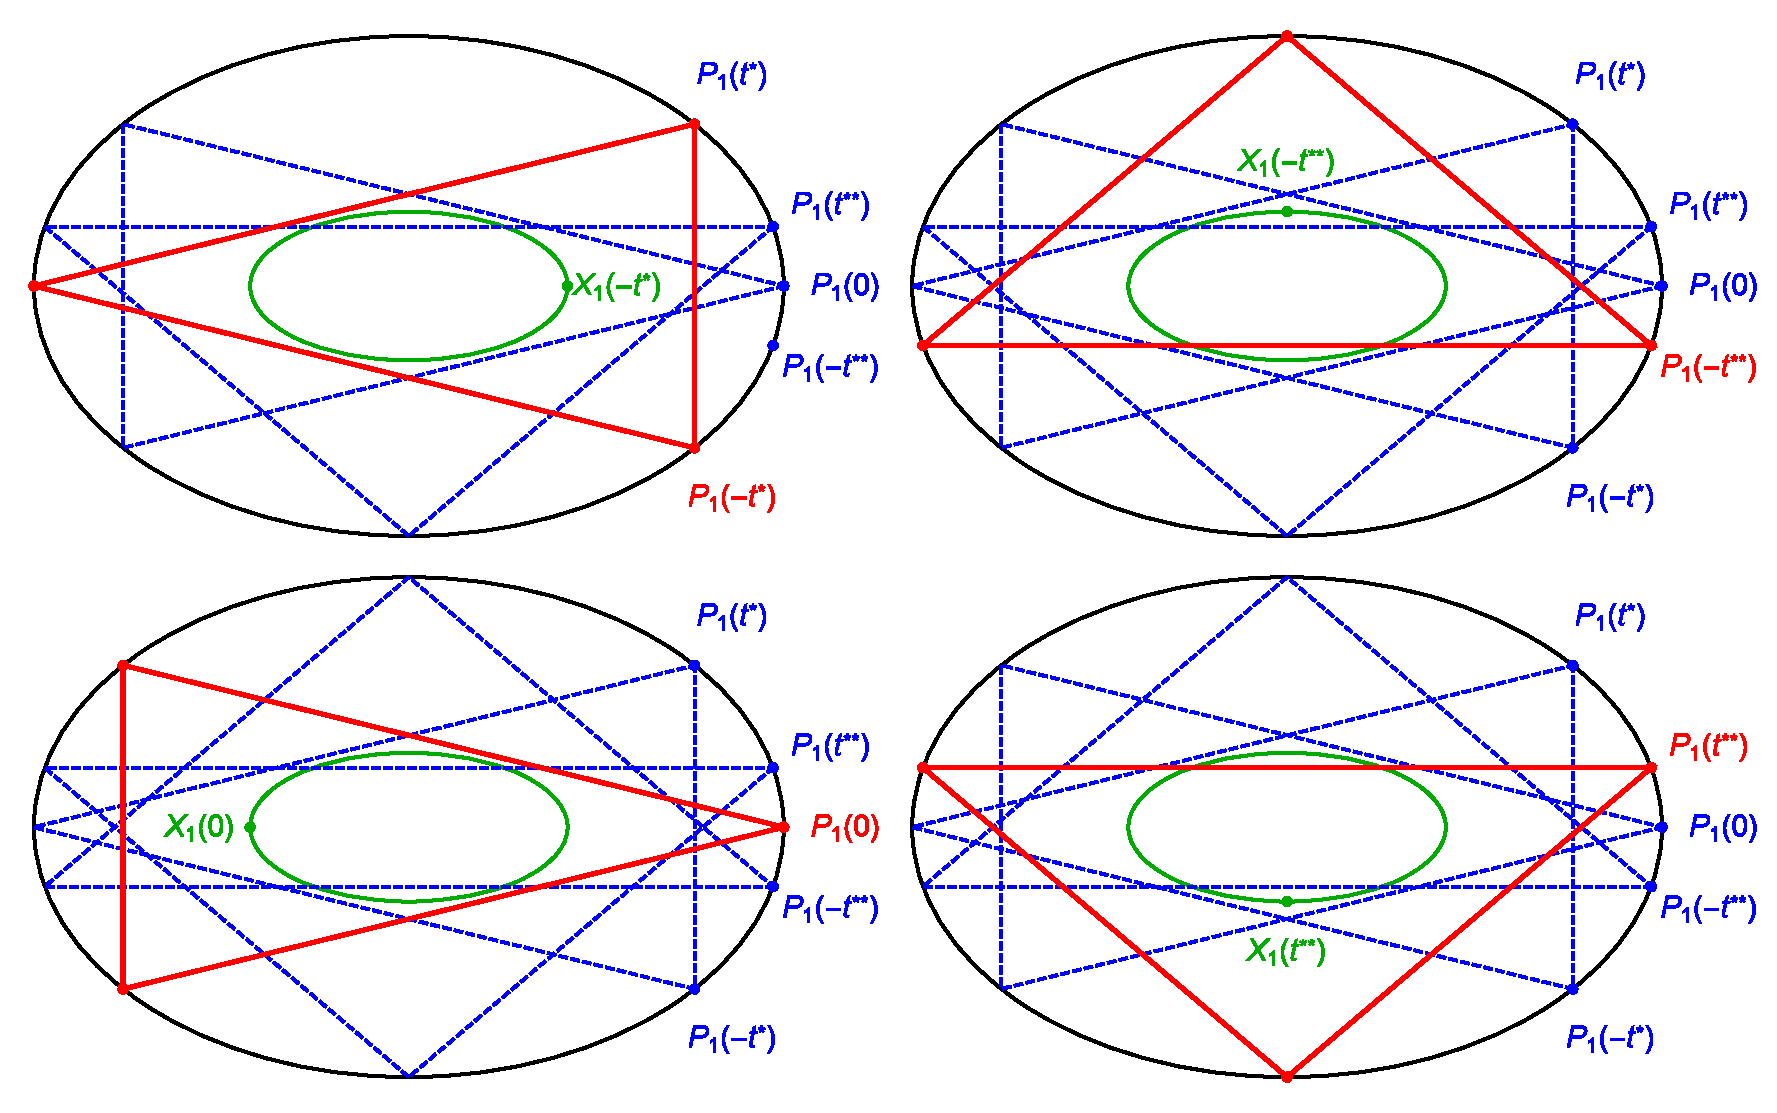
\includegraphics[width=.9\textwidth]{pics_1080_two_isosceles_tstar}
    \caption{Counterclockwise motion of $P_1(t)$, for $t=[-t^*,t^*)$ can be divided in four segments delimited by $t=(-t^*,-t^{**},0,t^{**},t^{**})$. Orbit positions for the first four are shown (red polygons) in the top-left, top-right, bot-left, and bot-right pictures. At $P_1({\pm}t^*)$ (resp.~$P_1({\pm}t^{**})$) the orbit is an isosceles triangle with a horizontal (resp.~vertical) axis of symmetry. Observations~\ref{obs:tstar1},\ref{obs:tstar2} assert that a counterclockwise motion of $P_1(t)$ along each of the four intervals causes a Triangle Center $X_i$ to execute a quarter turn along its locus (elliptic or not), and that a complete revolution of $P_1(t)$ around the EB causes $X_i$ to wind thrice on its locus. For illustration, the locus of $X_1(t)$ is shown (green) at each of the four interval endpoints.}
    \label{fig:triple-winding}
\end{figure}
Below we provide proofs of Lemmas \ref{lem:axis-of-symmetry}, \ref{lem:axisymmetric} and \ref{lem:center-cover}.
\begin{lemma*}[\ref{lem:axis-of-symmetry}]
Any Triangle Center $X_i$ of an isosceles triangle is on the axis of symmetry of said triangle.
\end{lemma*}

\begin{proof} Consider a sideways isosceles triangle with vertices $P_1=(x_1,0)$, $P_2=(-x_2,y_2)$
and $P_3= (-x_2,-y_2)$, i.e., its axis of symmetry is the $x$ axis. Let $X_i$ have Trilinears $p:q:r=h(s_1,s_2,s_3):h(s_2,s_3,s_1):h(s_3,s_1,s_2)$. Its Cartesians are given by Equation~\eqref{eqn:trilin-cartesian}. As $s_2=s_3$ and $h$ is symmetric on its last two variables $h(s_1,s_2,s_3)=h(s_1,s_3,s_2)$ it follows from equation \eqref{eqn:trilin-cartesian} that $y_i=0.$ %\textcolor{red}{ronaldo: can you provide more details.
%\textcolor{blue}{Mexi acima. Temos que melhorar os labels.}}
\end{proof}

\begin{lemma*}[\ref{lem:axisymmetric}]
If the locus of Triangle Center $X_i$ is elliptic, said ellipse must be concentric and axis-aligned with the EB.
\end{lemma*}

\begin{proof}
This follows from Lemma~\ref{lem:axisymmetric}.
\end{proof}


\begin{lemma*}[\ref{lem:center-cover}]
If the locus of $X_i$ is an ellipse, when $P_1(t)$ is at either EB vertex, its non-zero coordinate is equal to the corresponding locus semi-axis length.
\end{lemma*}

\begin{proof}
The family of 3-periodic orbits contains four isosceles triangles, Figure~\ref{fig:sideways-upright-orbit}. Parametrize $P_1(t)=(a\cos t,b\sin t)$. It follows from Lemma \ref{lem:axisymmetric} that $X_i(0)=(\pm a_i,0)$, $X_i(\pi/2)=(0,\pm b_i),$  $X_i(\pi)=(\mp a_i, 0)$ and $X_i(3\pi/2)=(0,\mp b_i)$, for some $a_i,b_i$. This ends the proof. %\textcolor{red}{ronaldo}
%\textcolor{blue}{Mexi so incluindo referencia ao lema 2 }
%Therefore, with $P_1(t)$ traveling the elliptic arc $\textrm{arc}[(a,0),(0,b)]$, $X_i(t)$ goes through one of the phases $\textrm{arc}[(\pm a_i,0),(0,\pm b_i)]$.
\end{proof}








% \section{Semiaxes of the 29 Elliptic Loci}
% \label{app:ell_axes}
% \input{app_103_ell_axes}

%\section{Table of Least-Squares}
%\label{app:least-squares-errors}
%\input{app_106_least_squares}

\section{Review: Early Observations}
\label{app:early}
Figure~\ref{fig:x12345-feuer-combo} (left) shows the elliptic loci of $X_k$, $k=1,...,5$. The latter two are new results.

\begin{figure}
\centering
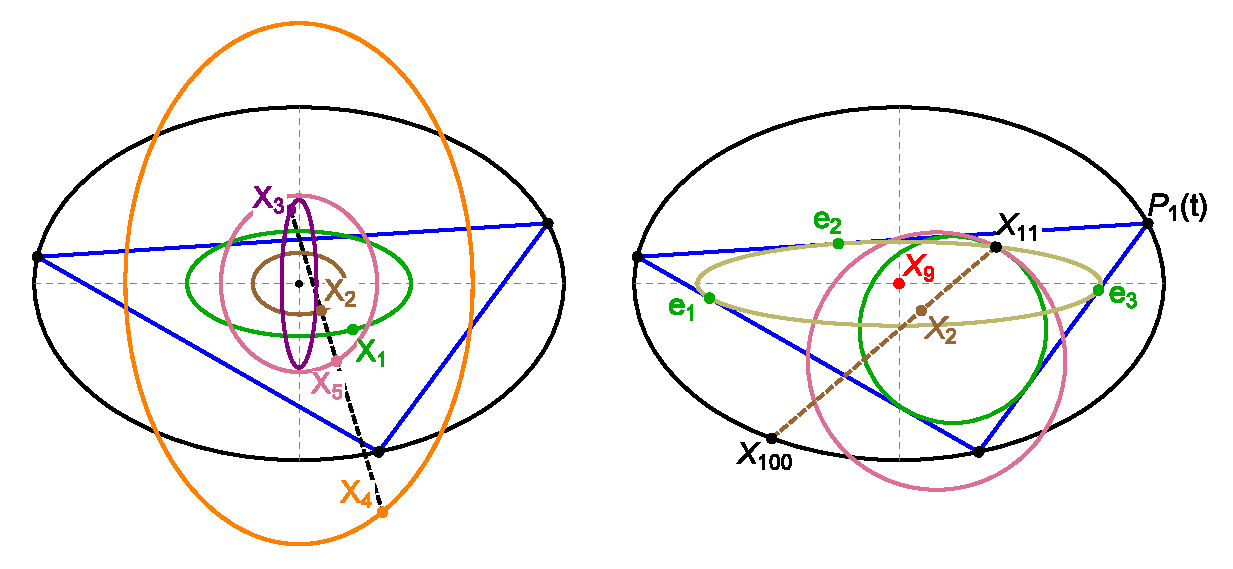
\includegraphics[width=\linewidth]{pics_1040_x12345_feuerbach_combo.eps}
\caption{\textbf{Left}: The loci of Incenter $X_1$, Barycenter $X_2$, Circumcenter $X_3$, Orthocenter $X_4$, and Center of the 9-Point Circle $X_5$ are all ellipses, \href{https://youtu.be/sMcNzcYaqtg}{Video}, \href{https://bit.ly/3opClJq}{app}. Also shown is the {\em Euler Line} (dashed black) which for any triangle, passes through all of $X_i$, $i=1...5$ \cite{mw}. \textbf{Right}: A 3-periodic orbit starting at $P_1(t)$ is shown (blue). The locus of $X_{11}$, where the Incircle (green) and 9-Point Circle (pink) meet, is the Caustic (brown), also swept by the Extouchpoints $e_i$. $X_{100}$ (double-length reflection of $X_{11}$ about $X_2$) is the EB \href{https://youtu.be/TXdg7tUl8lc}{Video}, \href{https://bit.ly/2LuARPo}{app}.}
\label{fig:x12345-feuer-combo}
\end{figure}

We have also observed that the locus of the Feuerbach Point $X_{11}$ coincides with the $N=3$ {\em Caustic}, a confocal ellipse to which the 3-periodic family is internally tangent, Appendix~\ref{app:billiards}. Additionally, the locus of $X_{100}$, the Anticomplement\footnote{Double-length reflection about the Centroid $X_2$.} of $X_{11}$ is the EB boundary. These phenomena appear in Figure~\ref{fig:x12345-feuer-combo} (right).

Indeed, some these facts will be known to triangle specialists if one regards the EB as the circumellipse centered on the Mittenpunkt $X_9$ \cite[X(9)]{etc} and \cite{dekov14}. For example, a full 57 Triangle Centers lie on said circumellipse. An animation of some of these points is viewable in \cite[pl\#10]{dsr_playlist_2020}.

\begin{figure}
 \begin{minipage}{\textwidth}
    \centering
    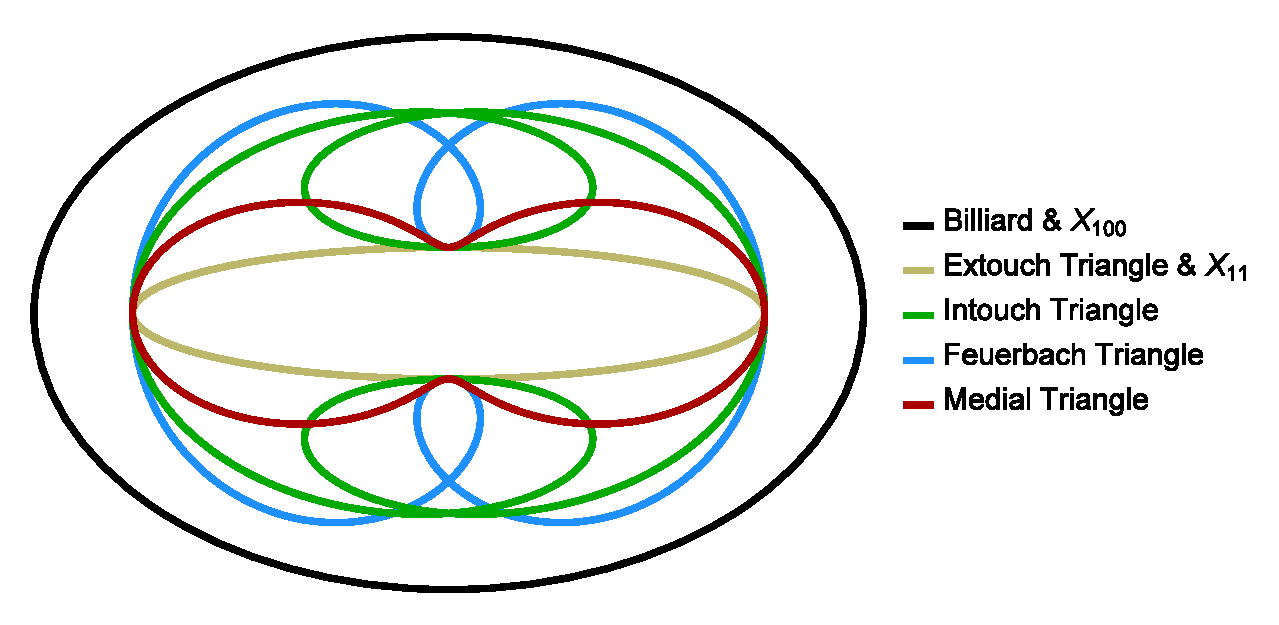
\includegraphics[width=.85\textwidth]{pics_1050_non_elliptic.eps}
    \caption[blablabla]{Loci generated by the vertices of selected orbit-Derived Triangles, namely: the Intouch (green), Feuerbach\footnote{Not to be confused with the Feuerbach Point $X_{11}$. The Feuerbach Triangle has vertices at the three contact points of the 9-point Circle with the Excircles \cite{mw}.} (blue), and Medial (red) Triangles are non-elliptic. However, those of the Extouch Triangle (brown), are identical to the $N=3$ Caustic (a curve also swept by $X_{11}$). Not shown is the locus of the Excentral Triangle, an ellipse similar to a rotated copy of the Incenter locus. \href{https://bit.ly/2MMH9e5}{app},
    \href{https://youtu.be/9xU6T7hQMzs}{Video 1}, \href{https://youtu.be/Xxr1DUo19_w}{Video 2}, \href{https://youtu.be/TXdg7tUl8lc}{Video 3}, \href{https://youtu.be/OGvCQbYqJyI}{Video 4}.}
    % tem q ficar aqui dentro do minipage!
    \label{fig:non-elliptic-vertex}
    \end{minipage}
\end{figure}

Additionally, a few  observations have been made \cite{reznik2020-intelligencer} about the loci of vertices of orbit-derived triangles (see Appendix~\ref{app:derived-tris}), some of which are elliptic and others non, illustrated in Figure~\ref{fig:non-elliptic-vertex}.


\end{document}  

